The presence of CPV can manifest itself through a nonzero value of the asymmetry defined as
\begin{linenomath}\begin{equation}\label{eq:counting_method}
    \Acp(\Oi) = \frac{\Npos-\Nneg}{\Npos+\Nneg},\quad i=3,\,6,\,12,\,14.
\end{equation}\end{linenomath}
The CP-violating asymmetries $\Acp(\Oi)$ are expected to vanish in the SM.
However, nonzero CP-violating couplings of the top quark from BSM phenomena can lead to sizable asymmetries.
An anomalous CEDM contribution~\cite{CPVtop:13TeVRef} can be as large as 8 and 0.4\% for $\Acp(\Othree)$ and $\Acp(\Otwelve)$, respectively.

Experimental factors, such as the misreconstruction of the physical objects, can affect the measurements of the asymmetries~\cite{CPVtop:13TeVRef}.
For example, misidentified signal events coming from \ttbar in the dilepton+jets channel can cause spurious asymmetry measurements.
We denote \Acp as the asymmetry that would be measured with an ideal detector and \Acpprime as the measured effective asymmetry, including experimental factors.
An estimate of \Acp can be obtained after correcting the measured asymmetry for instrumental effects.
Given that the SM predicts negligible \Acp in the top quark sector, a nonzero effective \Acpprime would be a strong hint of BSM phenomena.
For this reason, measurements of \Acpprime can be computed using \ttbar events and are the primary results presented in this paper.

Because \ttbar multijet events are highly suppressed by the signal-event requirements, only the \ttbar to lepton+jets and dilepton+jets channels are considered in the \ttbar contribution, with the latter assumed to be background.
The signal and background yields are determined through an extended maximum likelihood fit to the \Mlb distributions in data using simulated-event templates.
The \ttbar template is obtained from simulation, and the background template from the background-enriched events in data.
For each CP observable, the templates are classified according to the sign of the CP observable.
The extended likelihood function is defined as
\begin{linenomath}\begin{equation}\begin{aligned}
    L_{\text{ext}} &= \frac{\re^{-(\numpos+\ratiob \numb)}}{\Numpos!}\prod^{\Numpos}_{i=1} \numpos \fspos(\Mlbi) + \ratiob \numb \fbpos(\Mlbi) \\
    &+ \frac{\re^{-(\numneg+(1-\ratiob) \numb)}}{\Numneg!}\prod^{\Numneg}_{i=1} \numneg \fsneg(\Mlbi) + (1-\ratiob) \numb \fbneg(\Mlbi),
\end{aligned}\end{equation}\end{linenomath}
where \numb, \numpos, and \numneg are the parameters of interest and refer to the yields of background, and \ttbar events with positive and negative CP observable values, respectively; \ratiob refers to the fraction of background events with positive CP observable values obtained from the background template; $\fspos(\Mlb)$, $\fsneg(\Mlb)$, $\fbpos(\Mlb)$, and $\fbneg(\Mlb)$ refer to the probability density functions (pdf) of \Mlb obtained from the \ttbar and background templates according to the sign of the CP observable, respectively; and \Numpos and \Numneg are the number of events according to the sign of the CP observable.
To improve the fit results, the upper bound on \Mlb is relaxed to 500\GeV in the fit in order to include more sideband events.
However, to be consistent with the signal-event requirements, events with $\Mlb > 150\GeV$ are excluded after the fit in determining the final event yields for each CP observable.

Figures~\ref{fig:CR_SR_closure_test16},~\ref{fig:CR_SR_closure_test17},~\ref{fig:CR_SR_closure_test18} show the normalized \Mlb distributions from the signal and background-enriched events for the electron (left) and muon (right) channels.
The upper plots compare the distribution for the background-enriched data events to that from the MC prediction.
Good agreement is observed between the two distributions, showing that the background-enriched events are consistent with being entirely background.
The lower plots display the distributions for the background-enriched events in data and the predicted MC background in the signal-event sample.
The \Mlb distribution of background-enriched events in data is slightly wider than the predicted MC background in signal events.
This difference is taken as one of the systematic uncertainties, as discussed in Section~\ref{sec:uncertainty}.

\begin{figure}
    \centering
    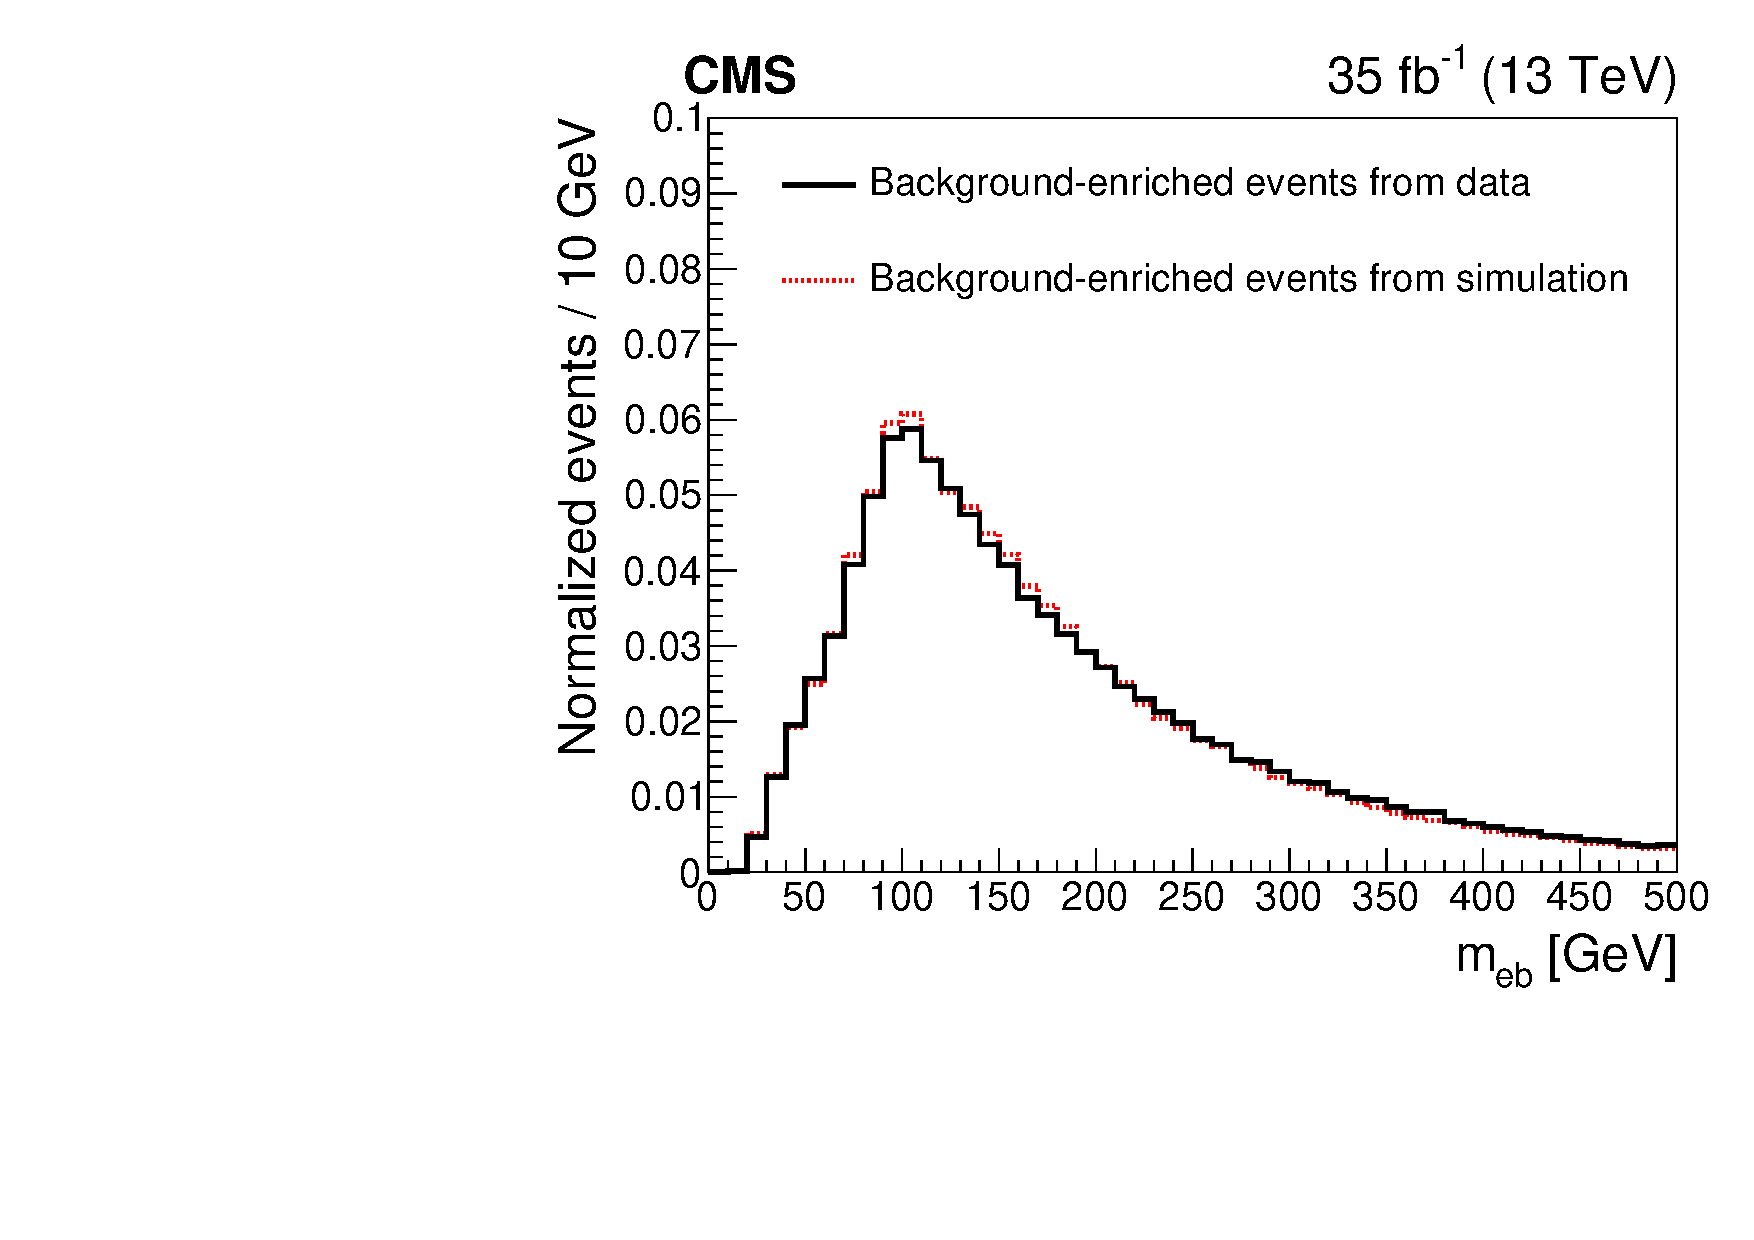
\includegraphics[width=0.45\textwidth]{figure/BGClosureTest_16_el_CR_chi2_20_wobtag.pdf}
    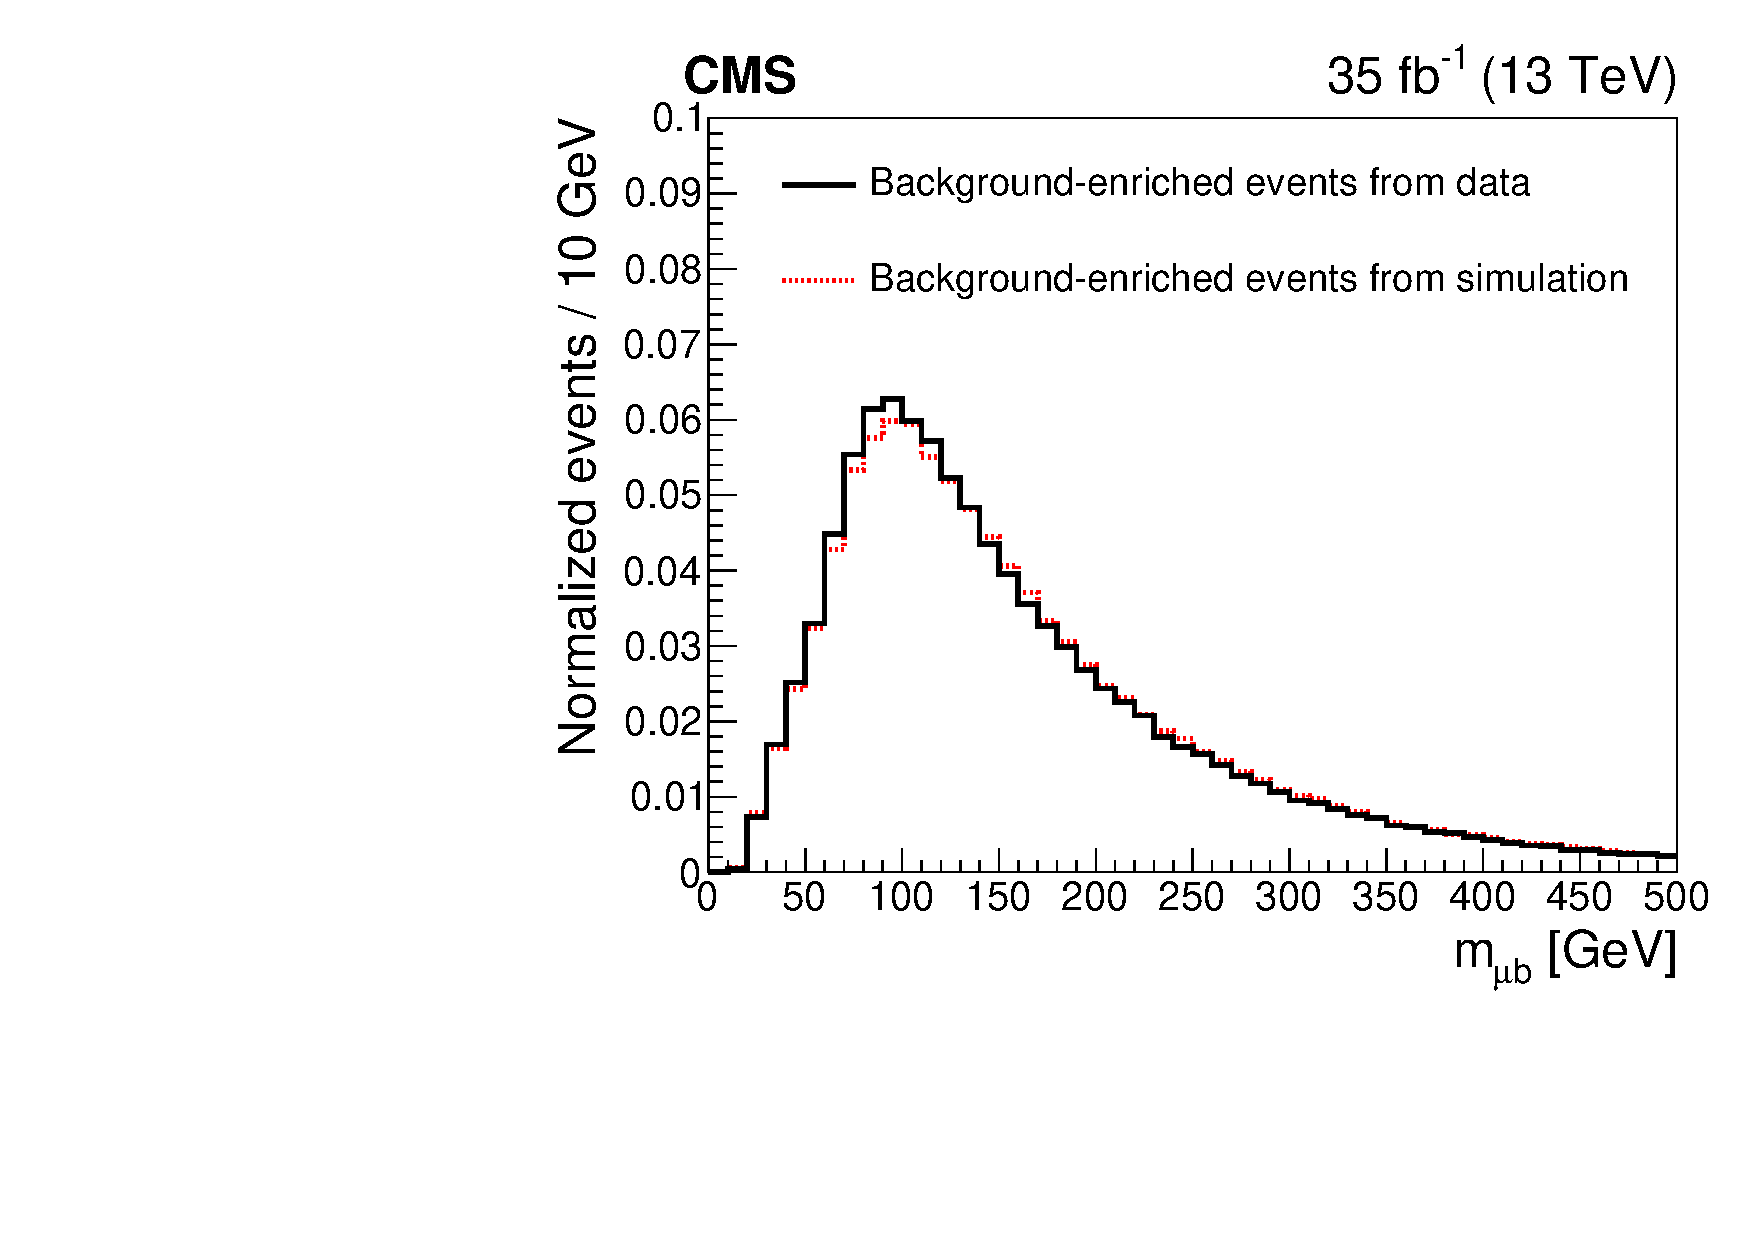
\includegraphics[width=0.45\textwidth]{figure/BGClosureTest_16_mu_CR_chi2_20_wobtag.pdf}
    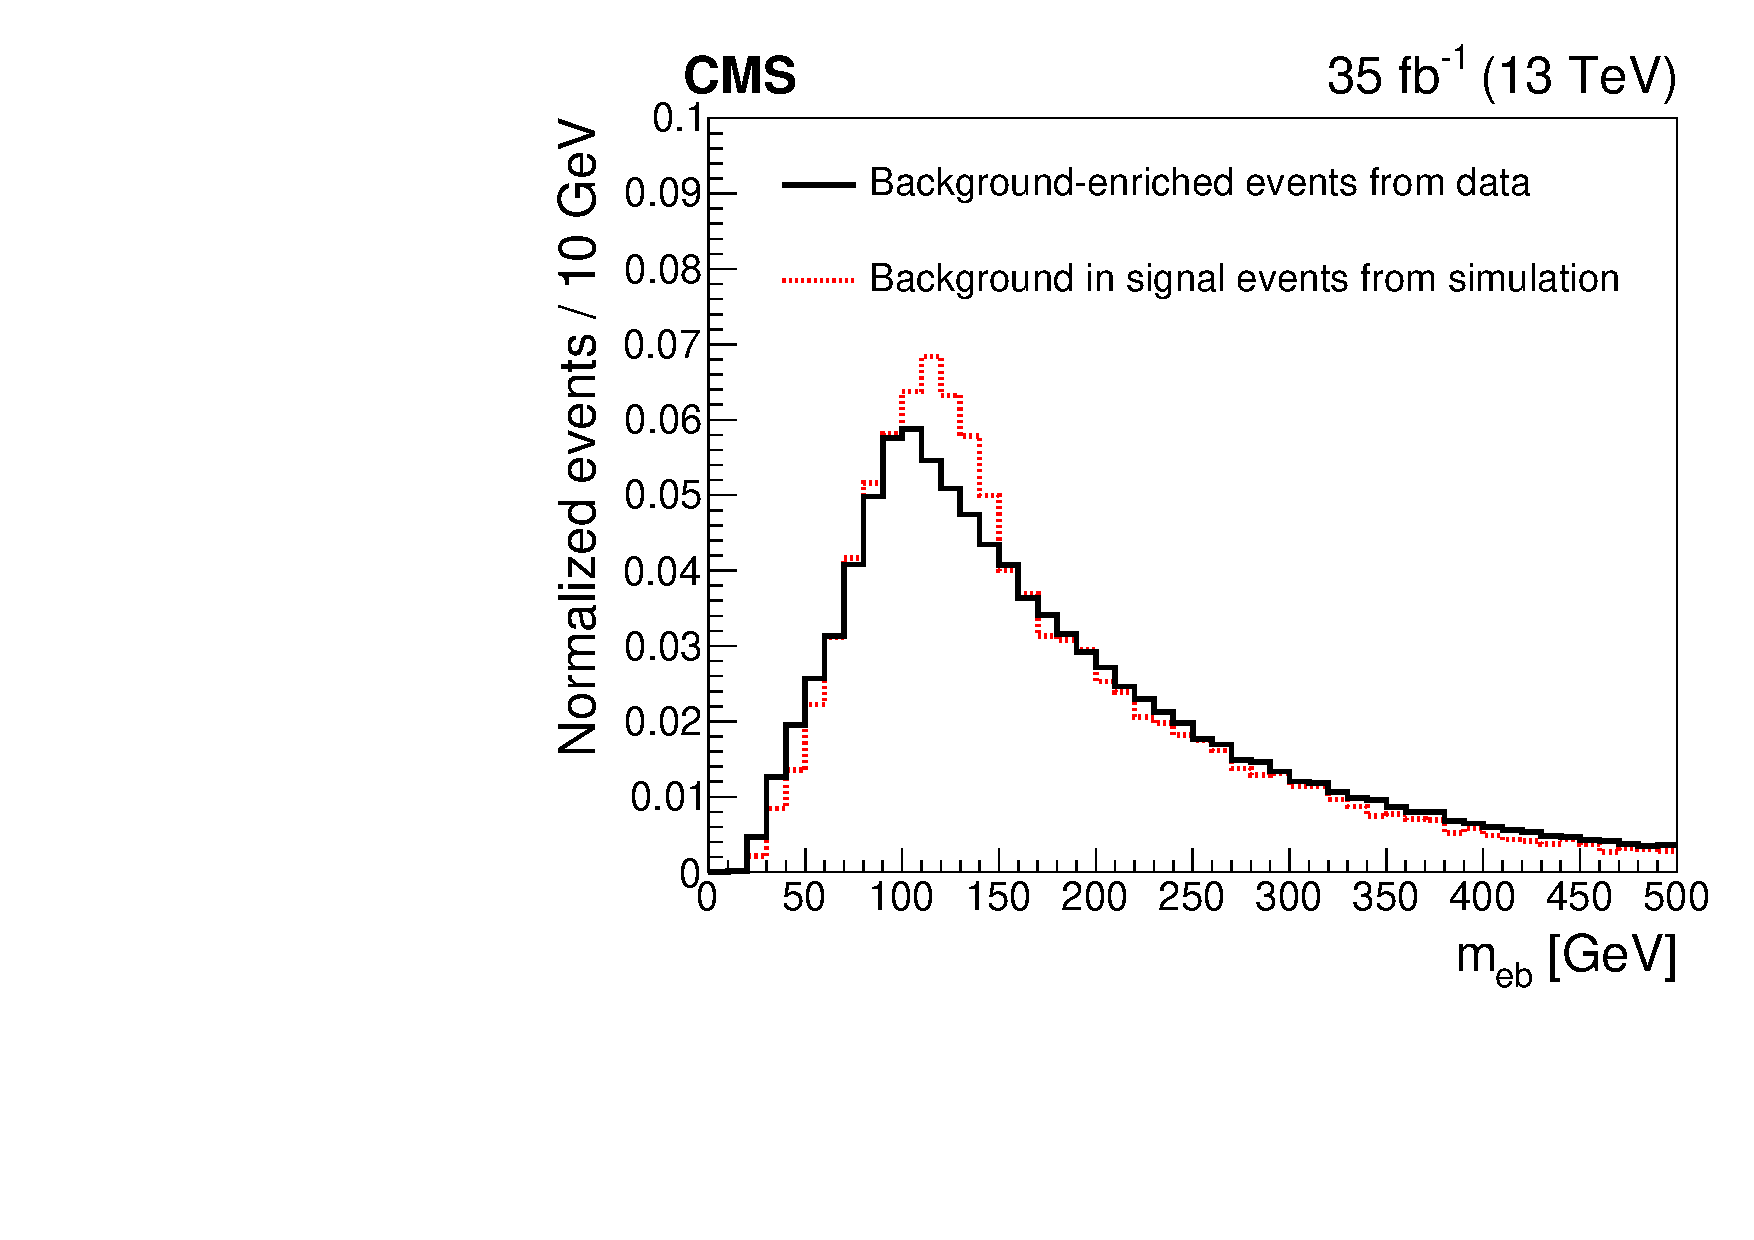
\includegraphics[width=0.45\textwidth]{figure/BGClosureTest_16_el_SR_chi2_20_wobtag.pdf}
    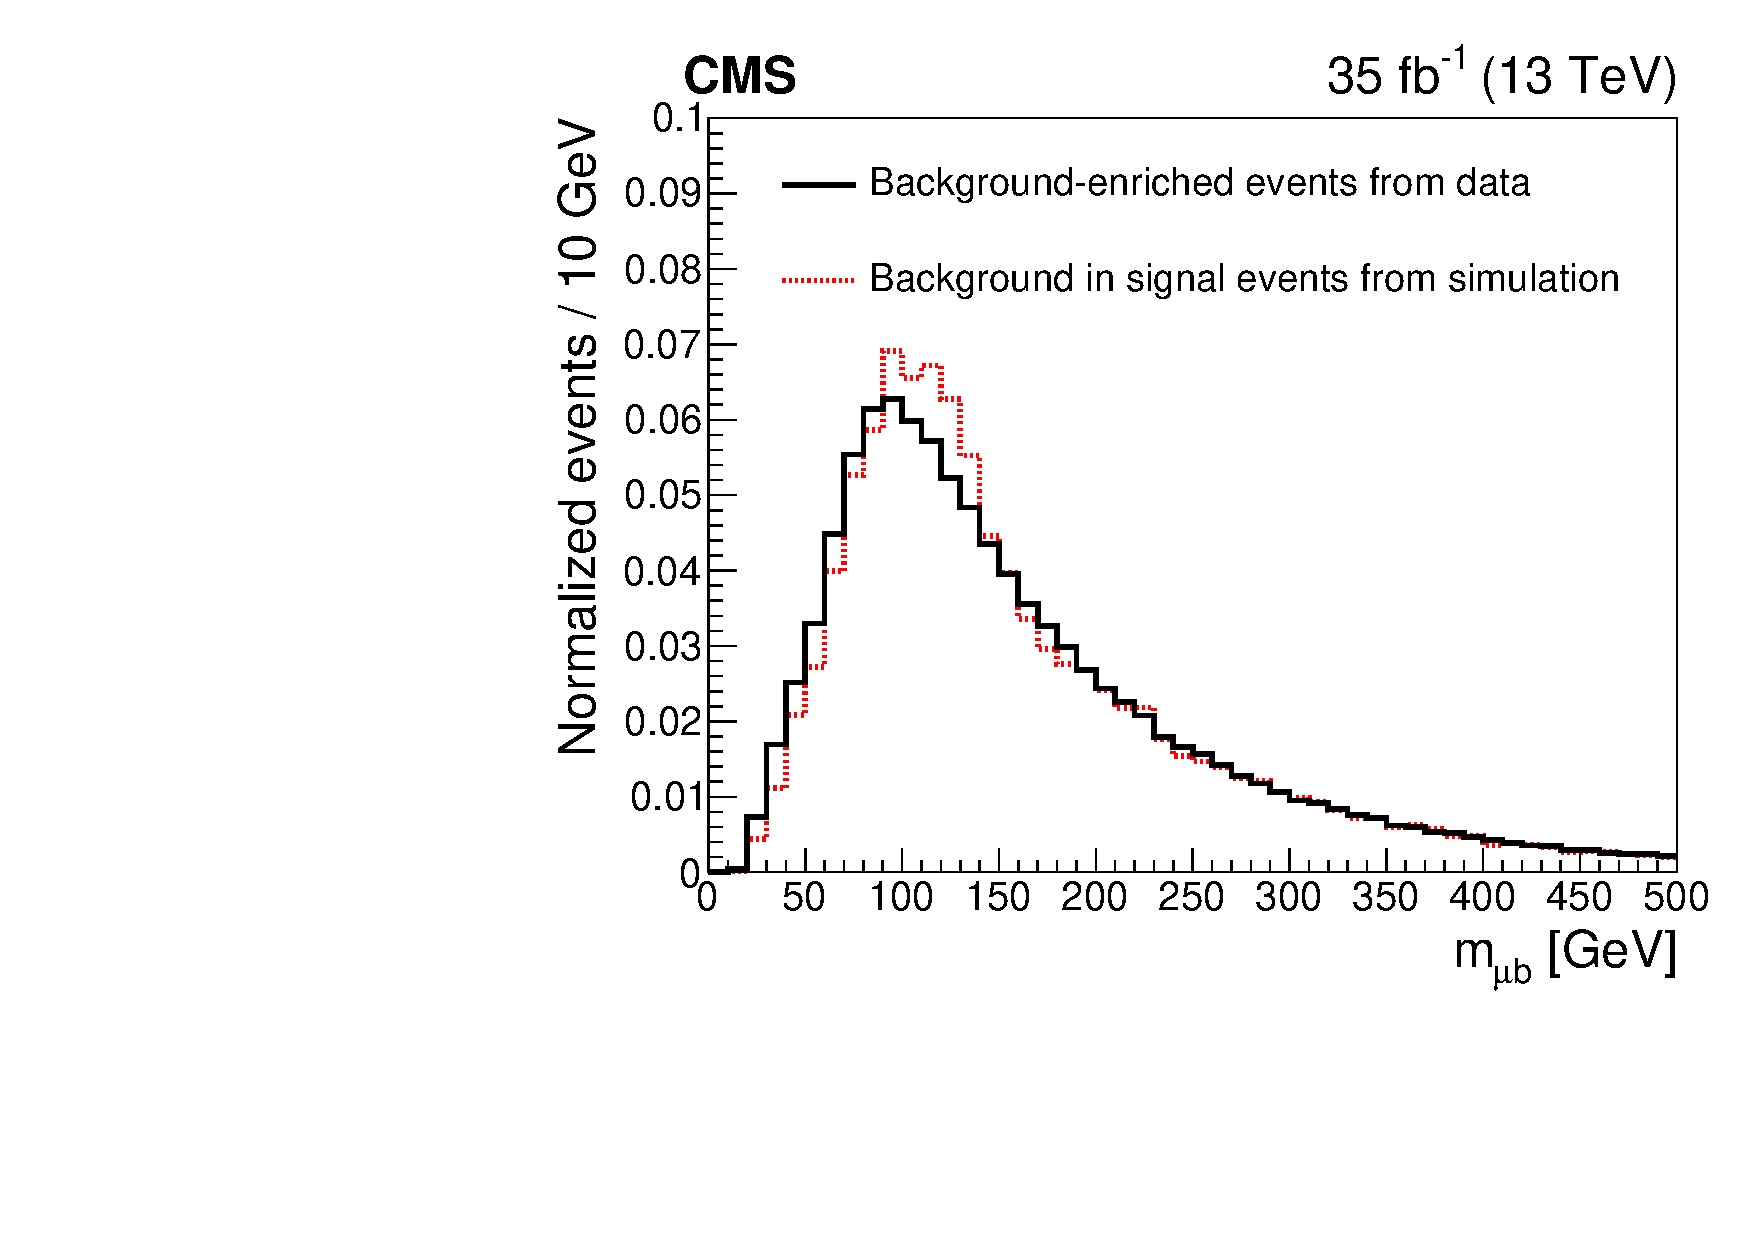
\includegraphics[width=0.45\textwidth]{figure/BGClosureTest_16_mu_SR_chi2_20_wobtag.pdf}
    \caption[The normalized \Mlb distributions in 2016 samples.]
    {
        The normalized \Mlb distributions for the electron (left) and muon (right) channels in 2016 samples.
        The upper two plots compare the background-enriched distributions from data (solid line) to the MC predictions (dotted-red line).
        The lower two plots give the background-enriched distributions from data (solid line) and the MC predictions for the distributions from the background in the signal events.
    }
    \label{fig:CR_SR_closure_test16}
\end{figure}

\begin{figure}
    \centering
    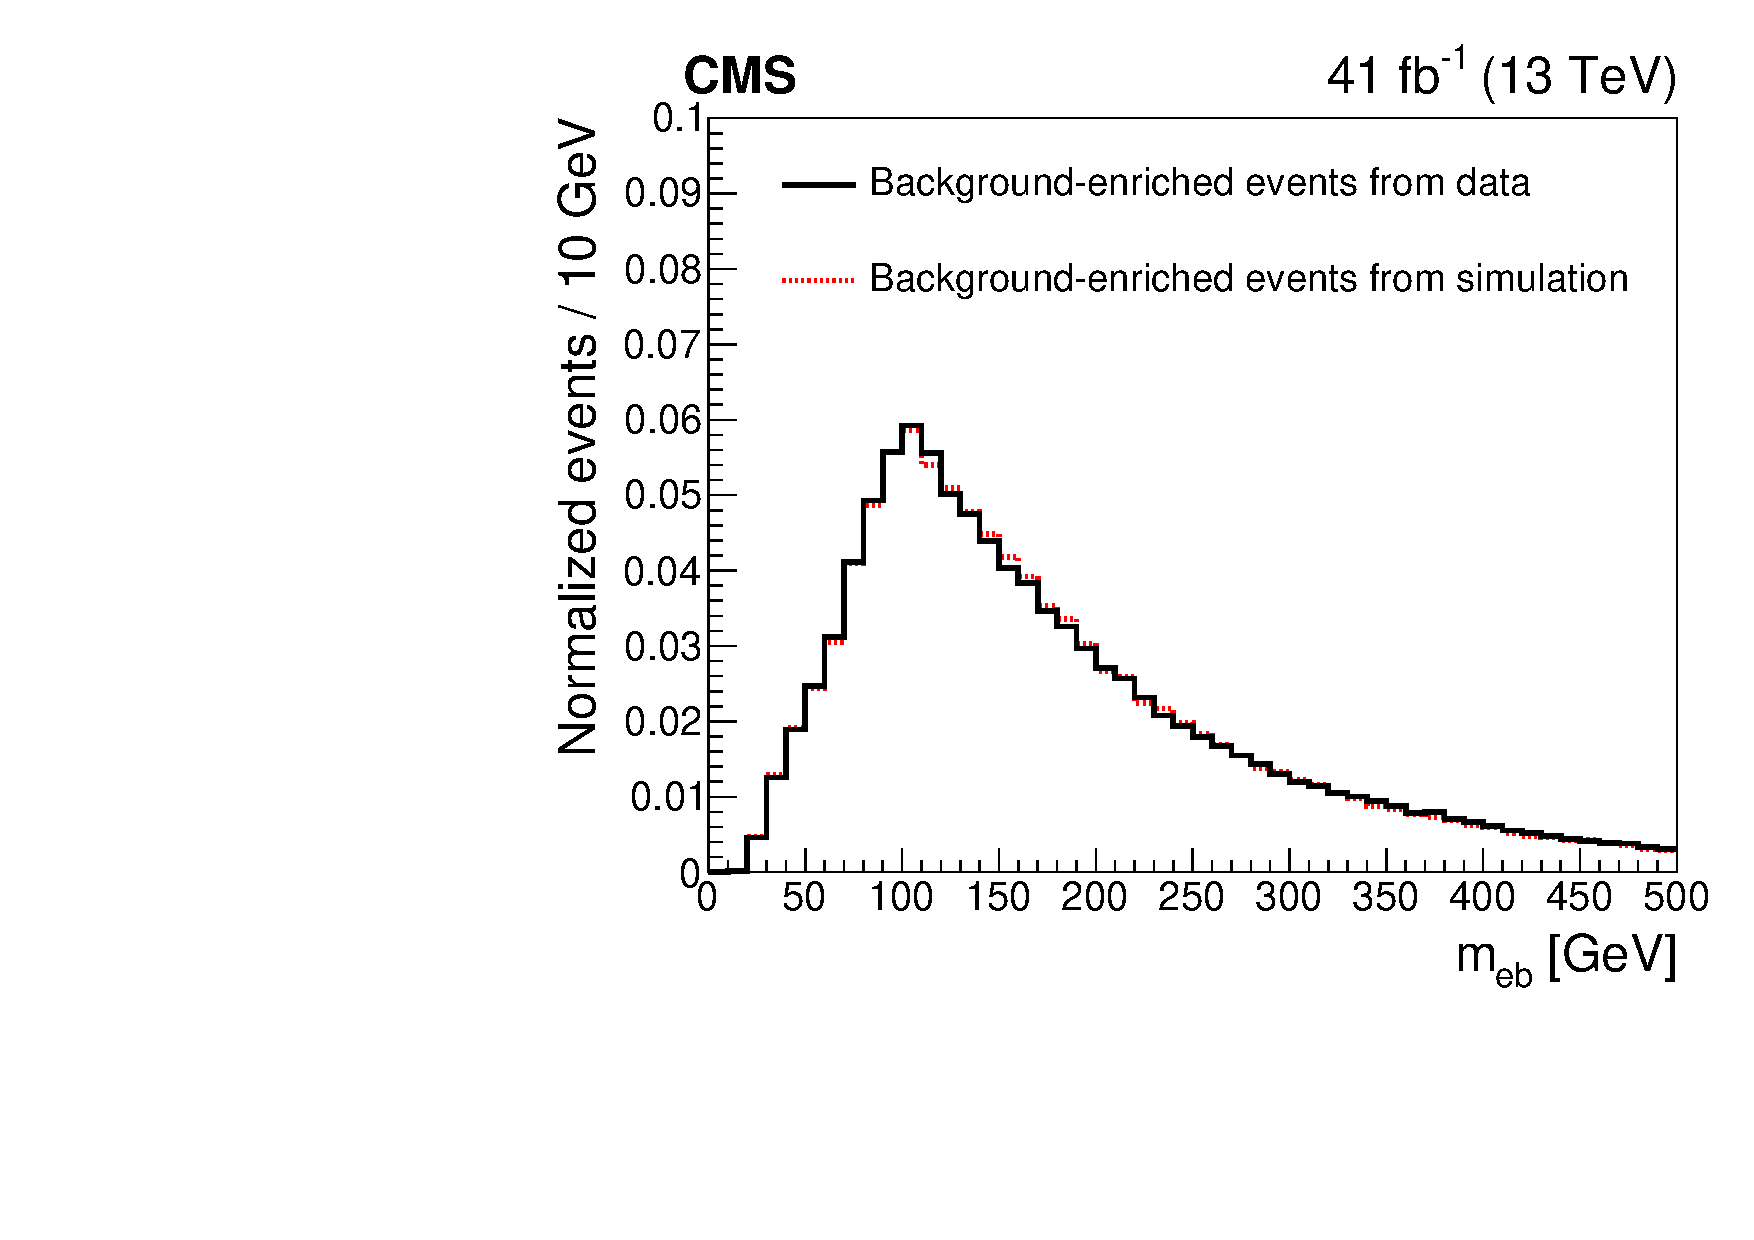
\includegraphics[width=0.45\textwidth]{figure/BGClosureTest_17_el_CR_chi2_20_wobtag.pdf}
    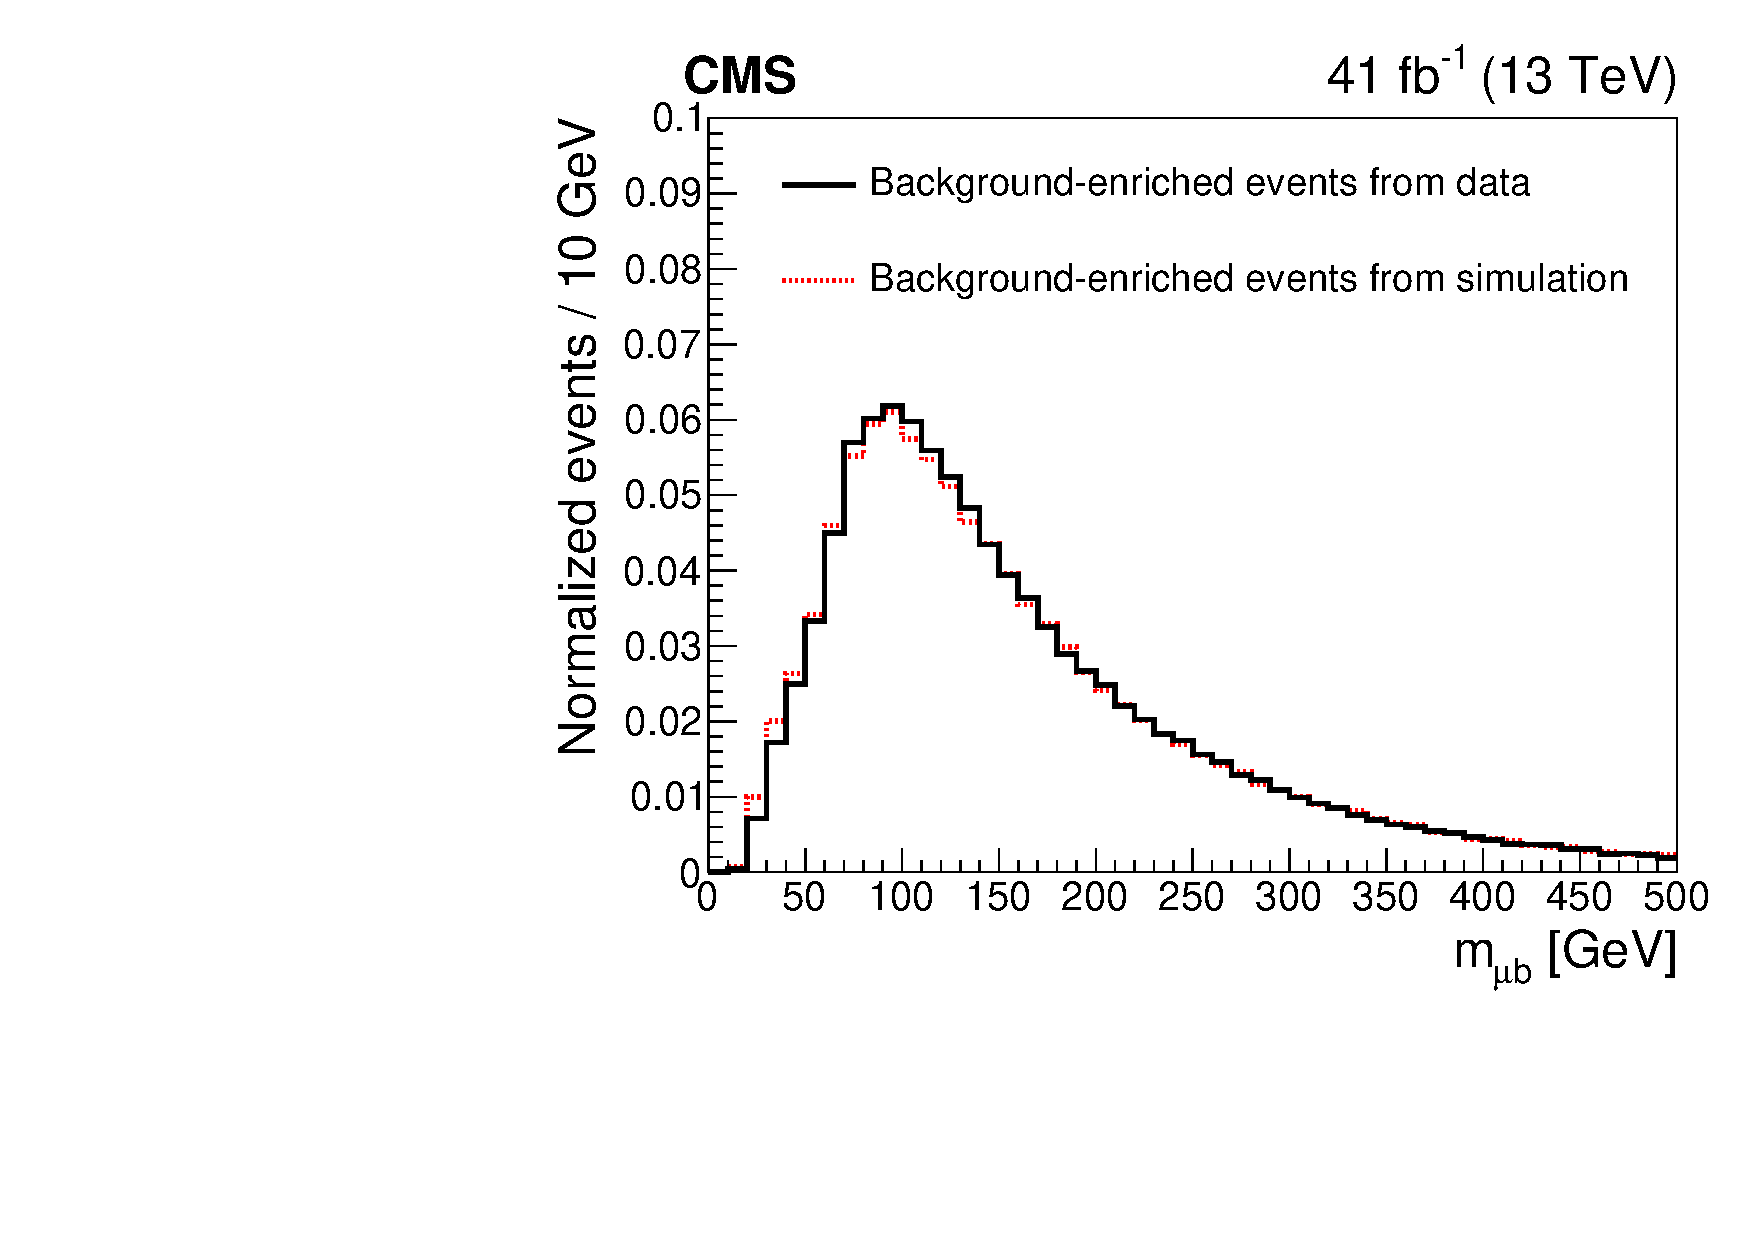
\includegraphics[width=0.45\textwidth]{figure/BGClosureTest_17_mu_CR_chi2_20_wobtag.pdf}
    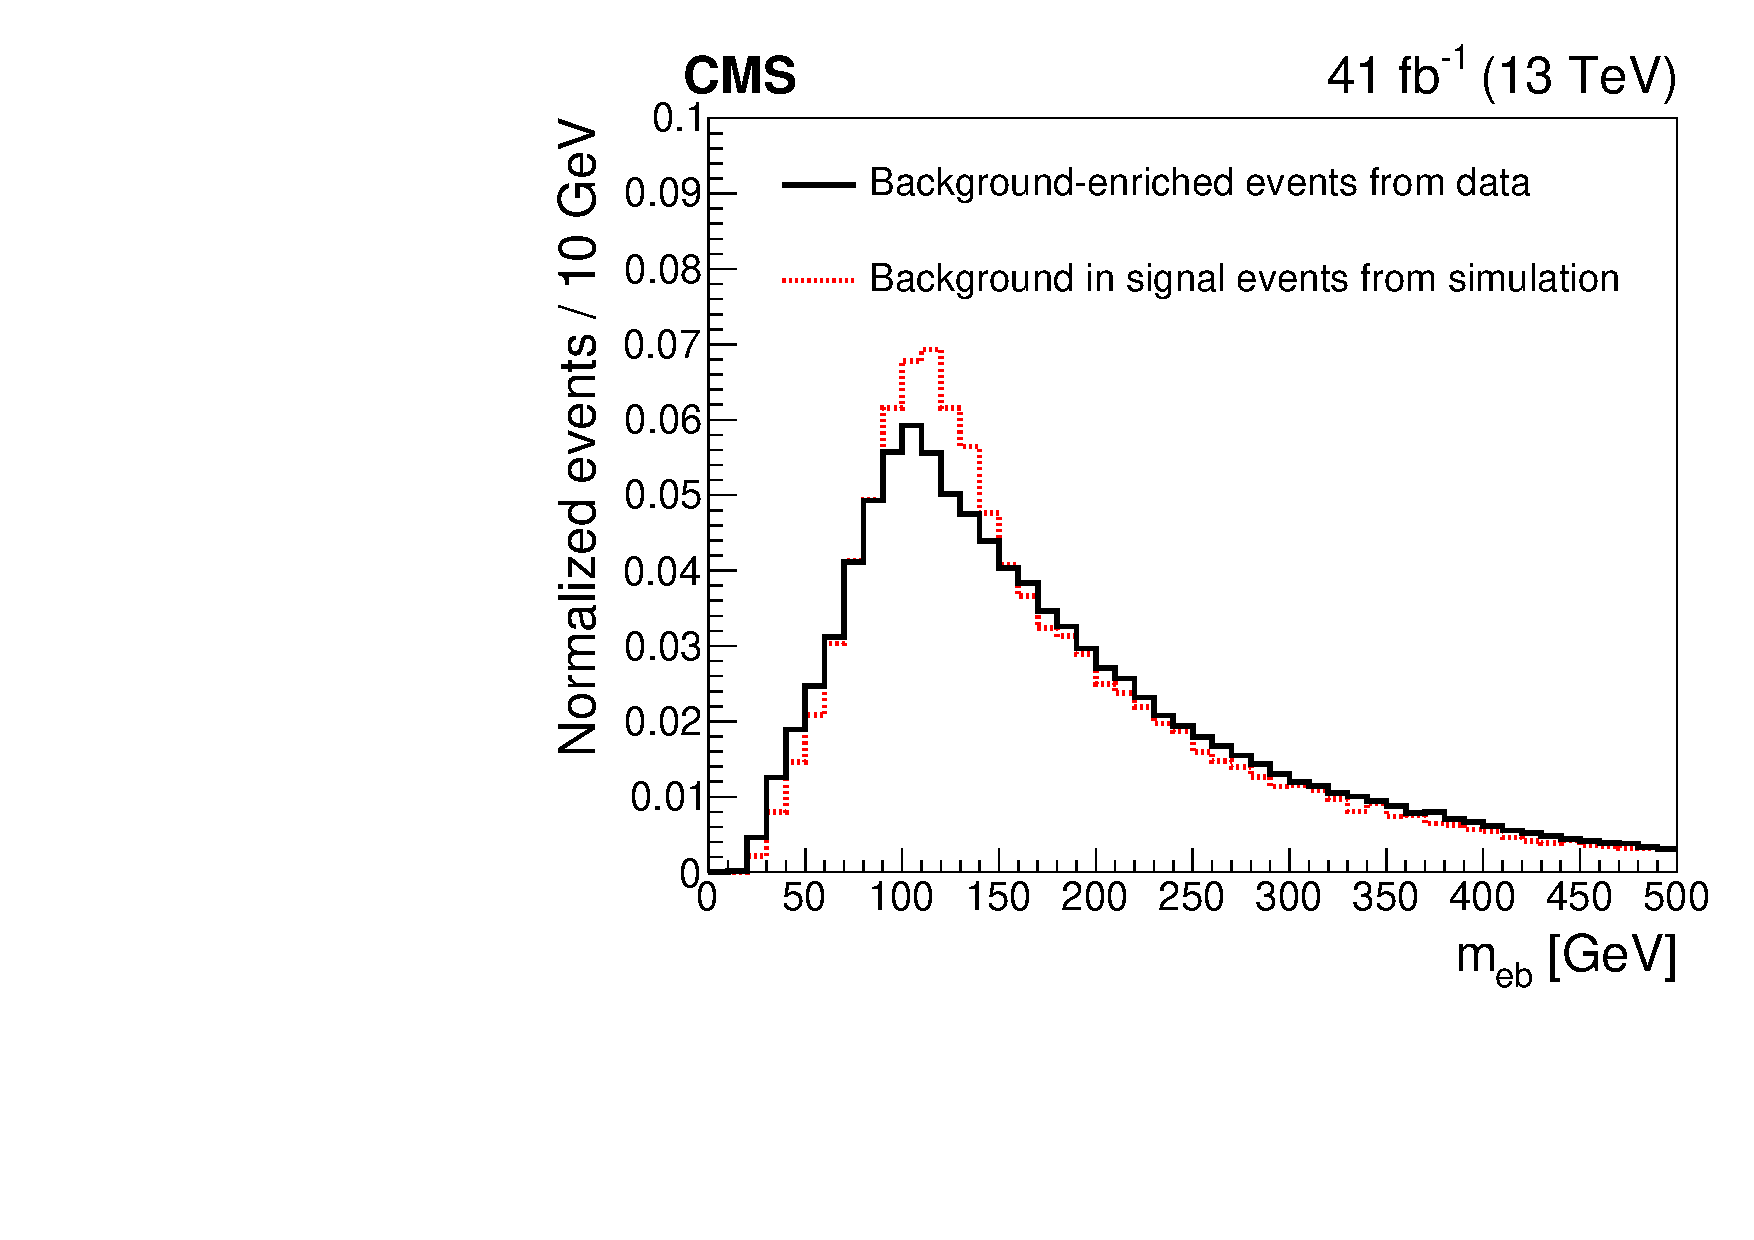
\includegraphics[width=0.45\textwidth]{figure/BGClosureTest_17_el_SR_chi2_20_wobtag.pdf}
    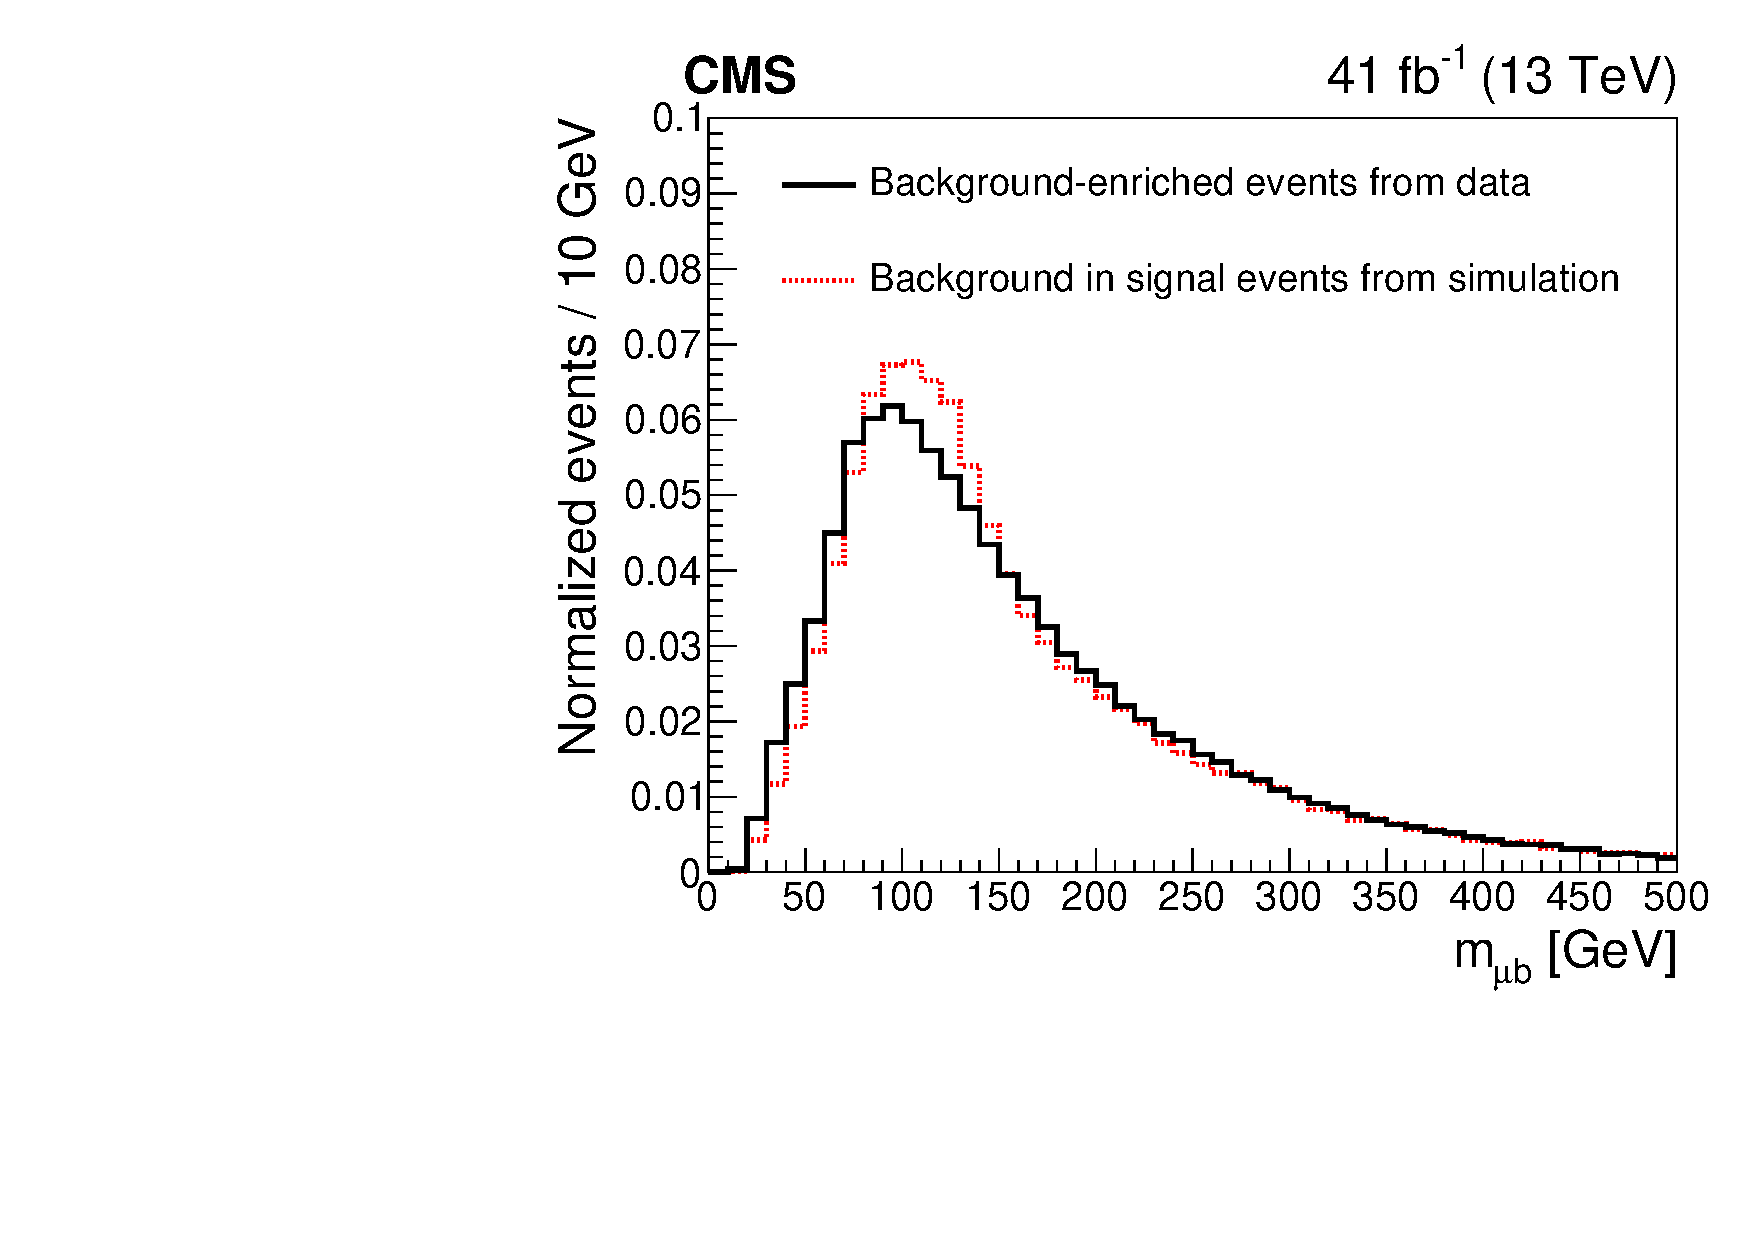
\includegraphics[width=0.45\textwidth]{figure/BGClosureTest_17_mu_SR_chi2_20_wobtag.pdf}
    \caption[The normalized \Mlb distributions in 2017 samples.]
    {
        The normalized \Mlb distributions for the electron (left) and muon (right) channels in 2017 samples.
        The upper two plots compare the background-enriched distributions from data (solid line) to the MC predictions (dotted-red line).
        The lower two plots give the background-enriched distributions from data (solid line) and the MC predictions for the distributions from the background in the signal events.
    }
    \label{fig:CR_SR_closure_test17}
\end{figure}

\begin{figure}
    \centering
    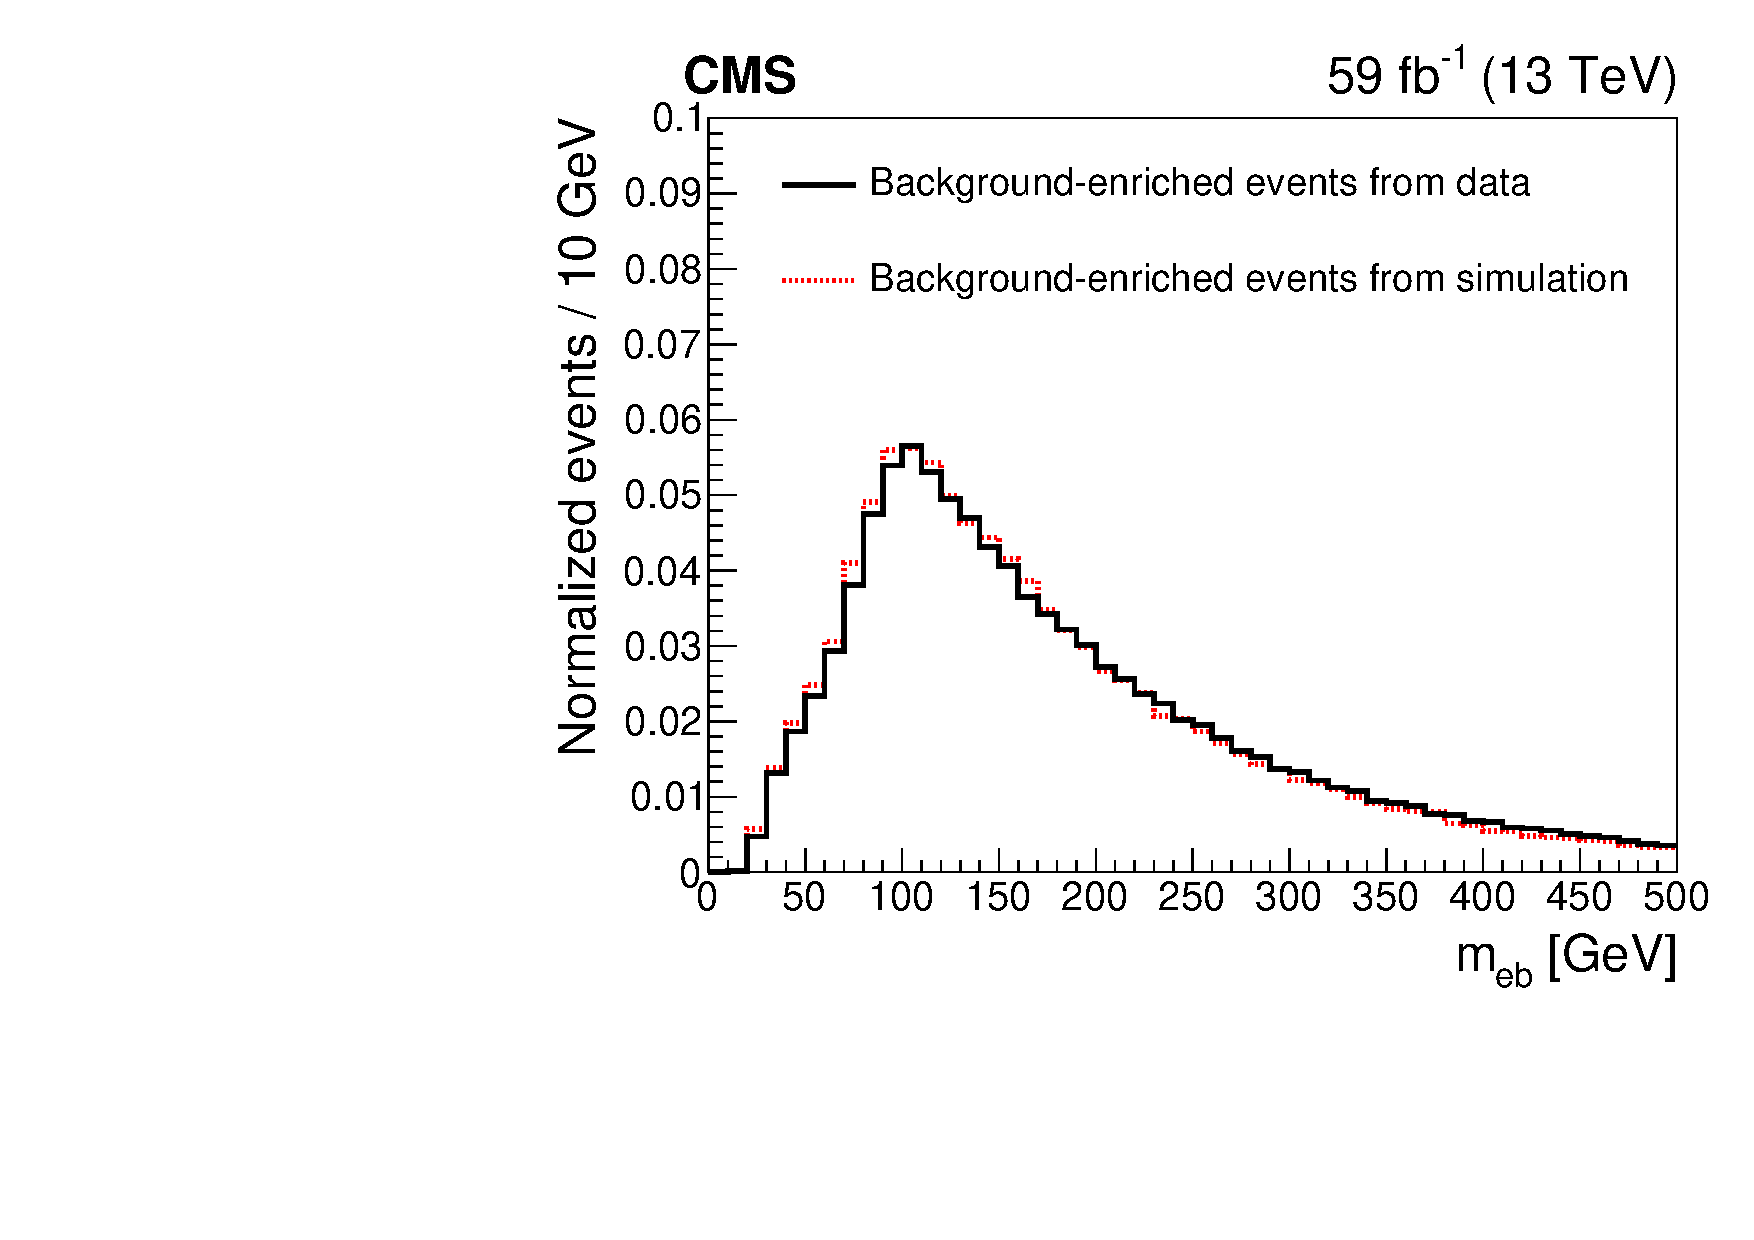
\includegraphics[width=0.45\textwidth]{figure/BGClosureTest_18_el_CR_chi2_20_wobtag.pdf}
    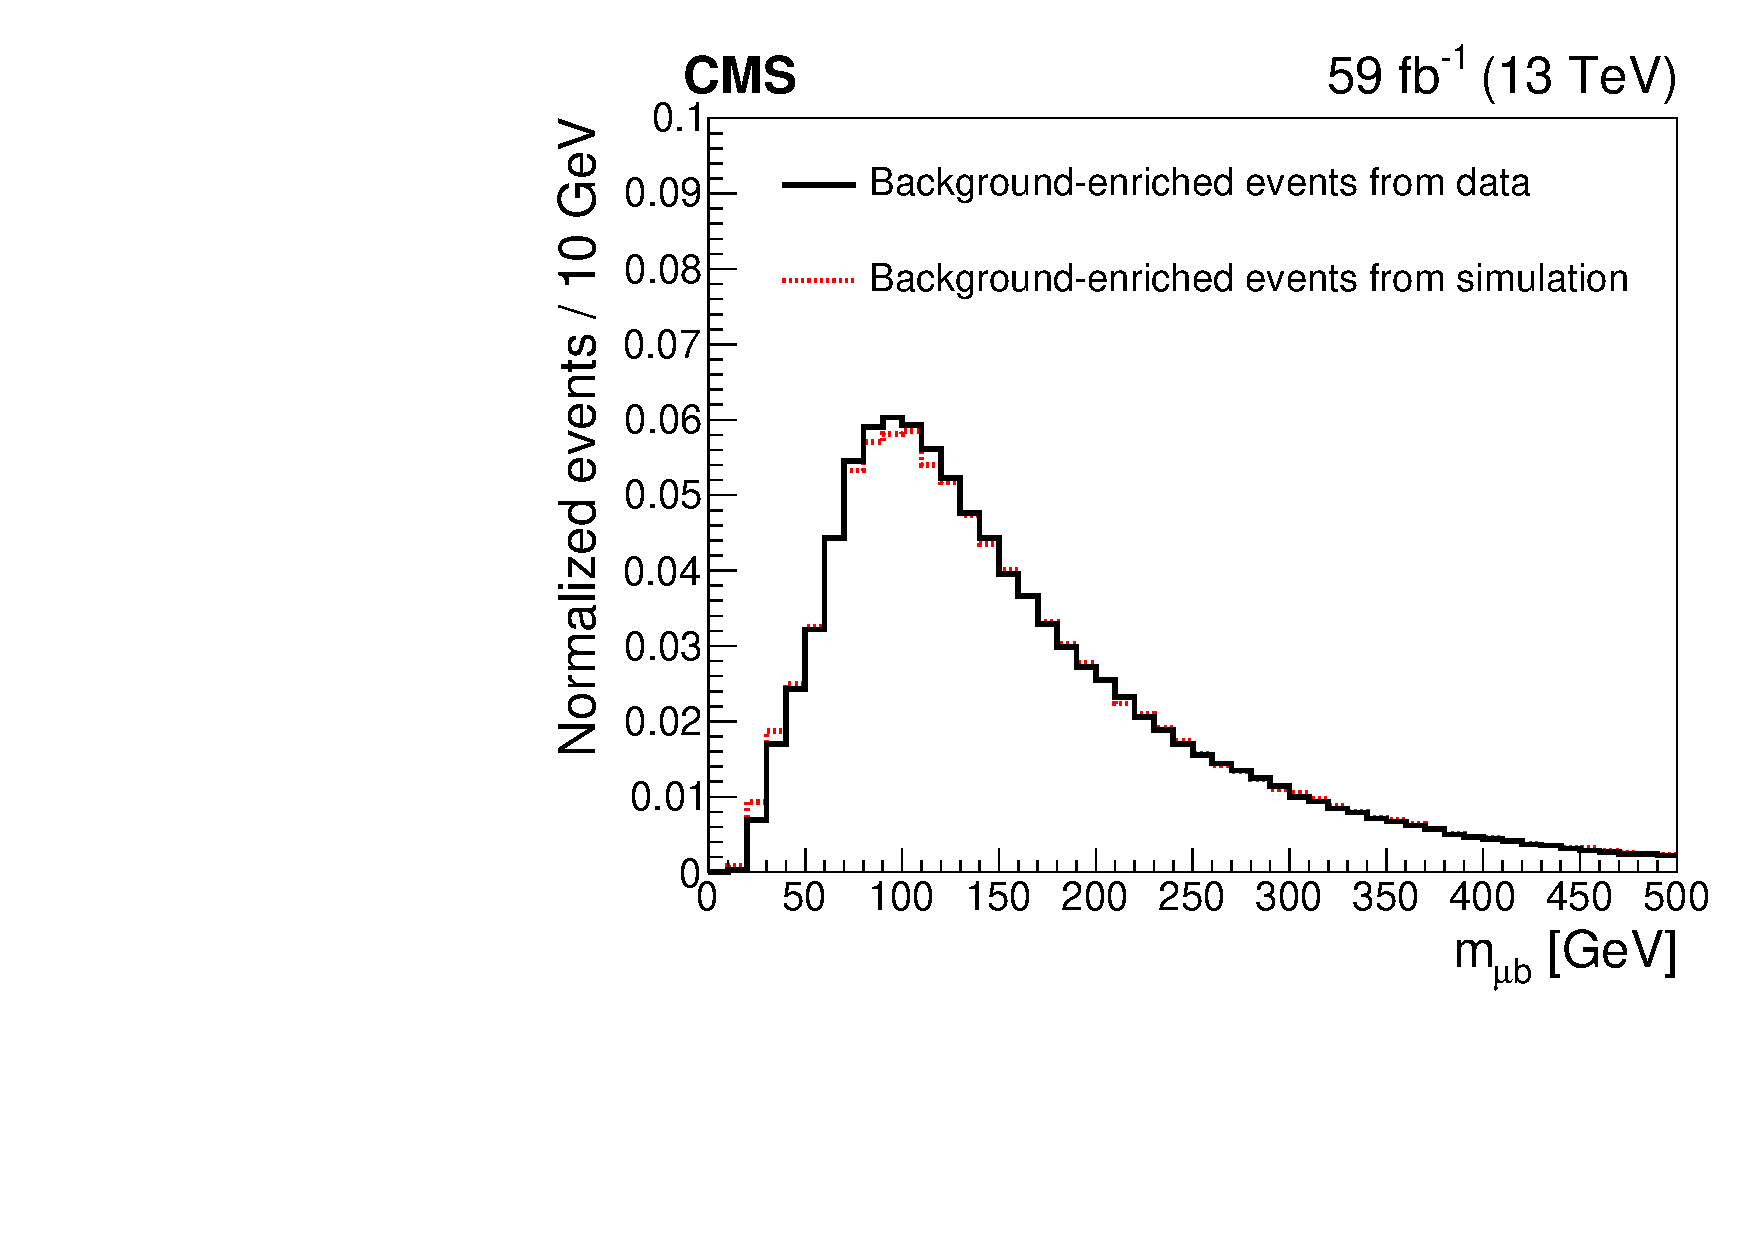
\includegraphics[width=0.45\textwidth]{figure/BGClosureTest_18_mu_CR_chi2_20_wobtag.pdf}
    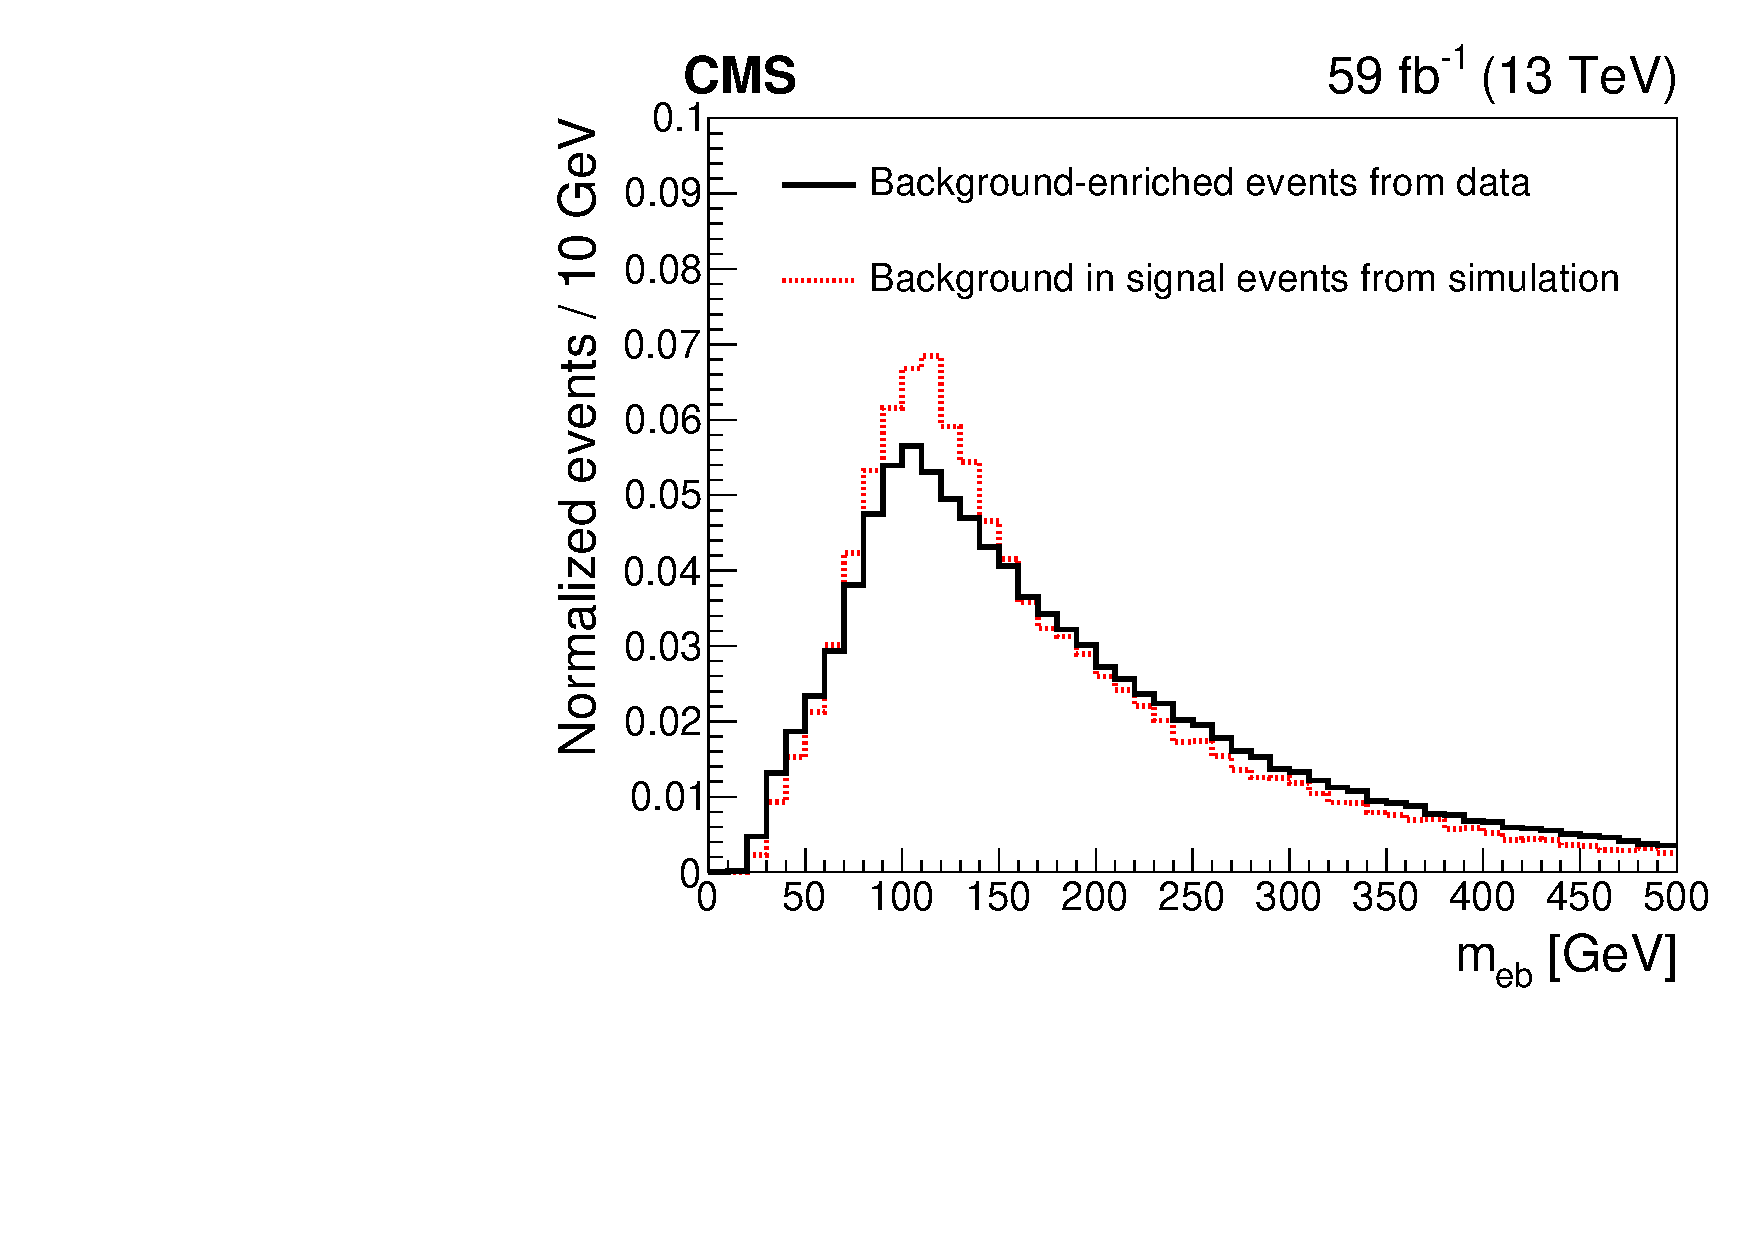
\includegraphics[width=0.45\textwidth]{figure/BGClosureTest_18_el_SR_chi2_20_wobtag.pdf}
    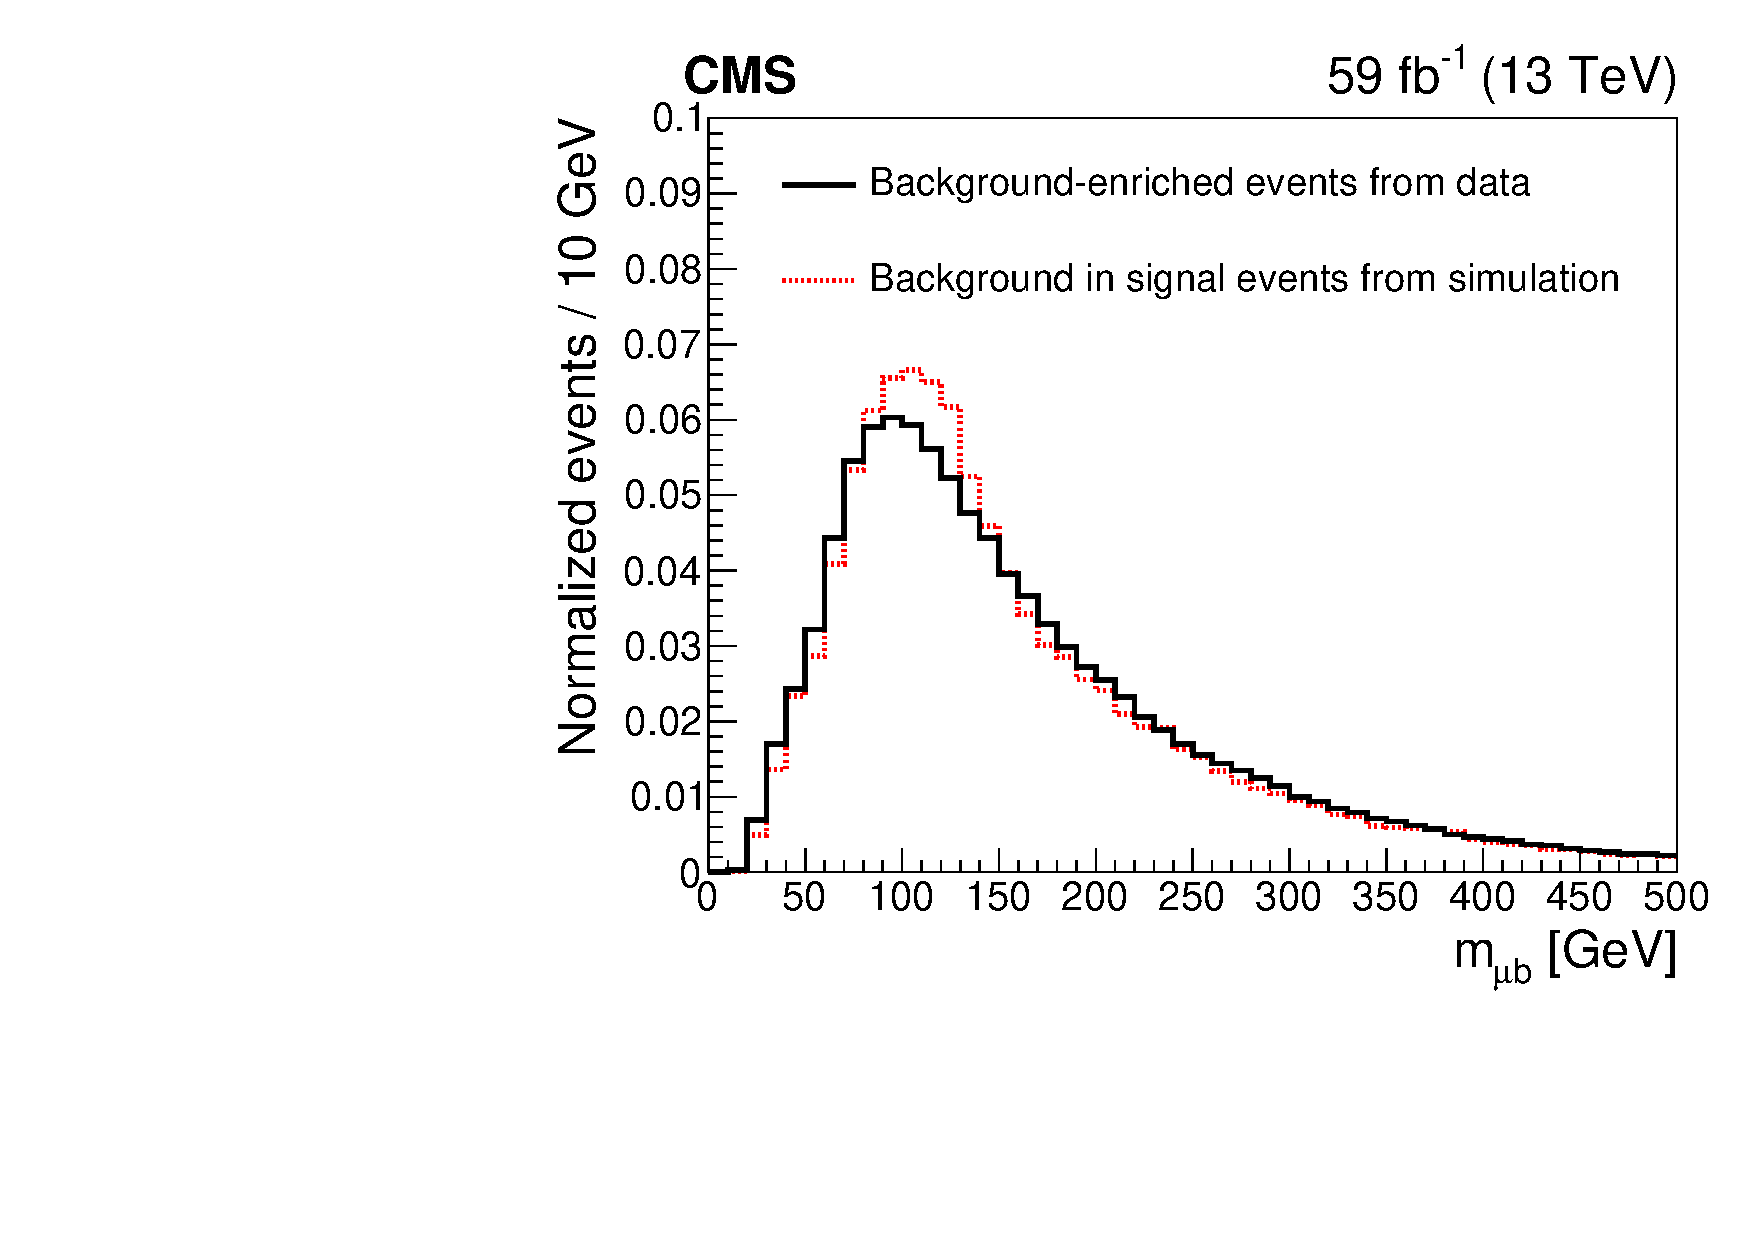
\includegraphics[width=0.45\textwidth]{figure/BGClosureTest_18_mu_SR_chi2_20_wobtag.pdf}
    \caption[The normalized \Mlb distributions in 2018 samples.]
    {
        The normalized \Mlb distributions for the electron (left) and muon (right) channels in 2018 samples.
        The upper two plots compare the background-enriched distributions from data (solid line) to the MC predictions (dotted-red line).
        The lower two plots give the background-enriched distributions from data (solid line) and the MC predictions for the distributions from the background in the signal events.
    }
    \label{fig:CR_SR_closure_test18}
\end{figure}

The \Mlb distributions in data per year are shown in Figs.~\ref{fig:fitting_results_16_el},~\ref{fig:fitting_results_16_mu},~\ref{fig:fitting_results_17_el},~\ref{fig:fitting_results_17_mu},~\ref{fig:fitting_results_18_el},~\ref{fig:fitting_results_18_mu} along with the results of the fit.
The combined measured numbers of \ttbar signal and background events in the electron and muon channels from the fits, and the corresponding \ttbar purities, are presented in Table~\ref{tab:fitting_purity}.
The final \Acpprime measurements can then be computed using the event-counting method of Eq.~\eqref{eq:counting_method}.
\begin{figure}
    \centering
    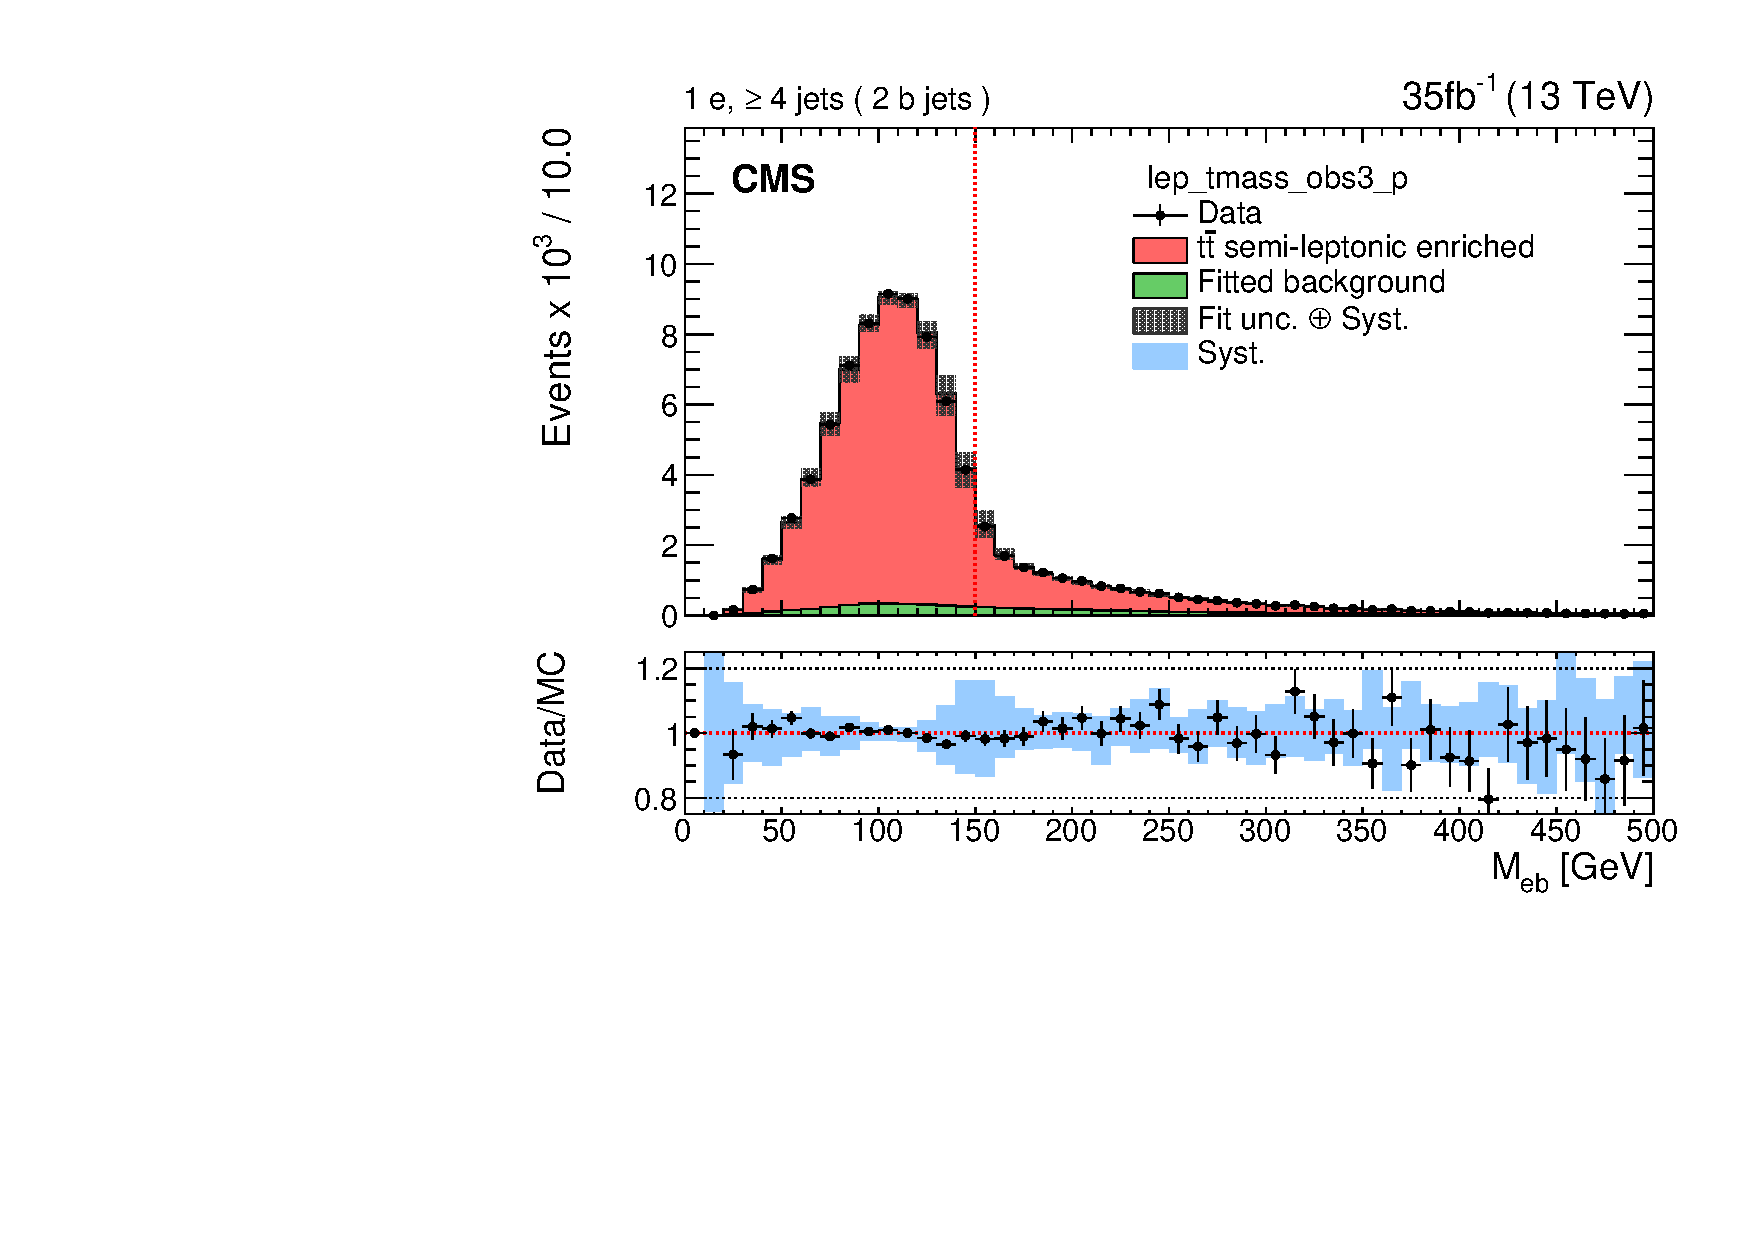
\includegraphics[width=0.4\textwidth]{figure/FitResult_16_el_lep_tmass_obs3_p_chi2_20.pdf}
    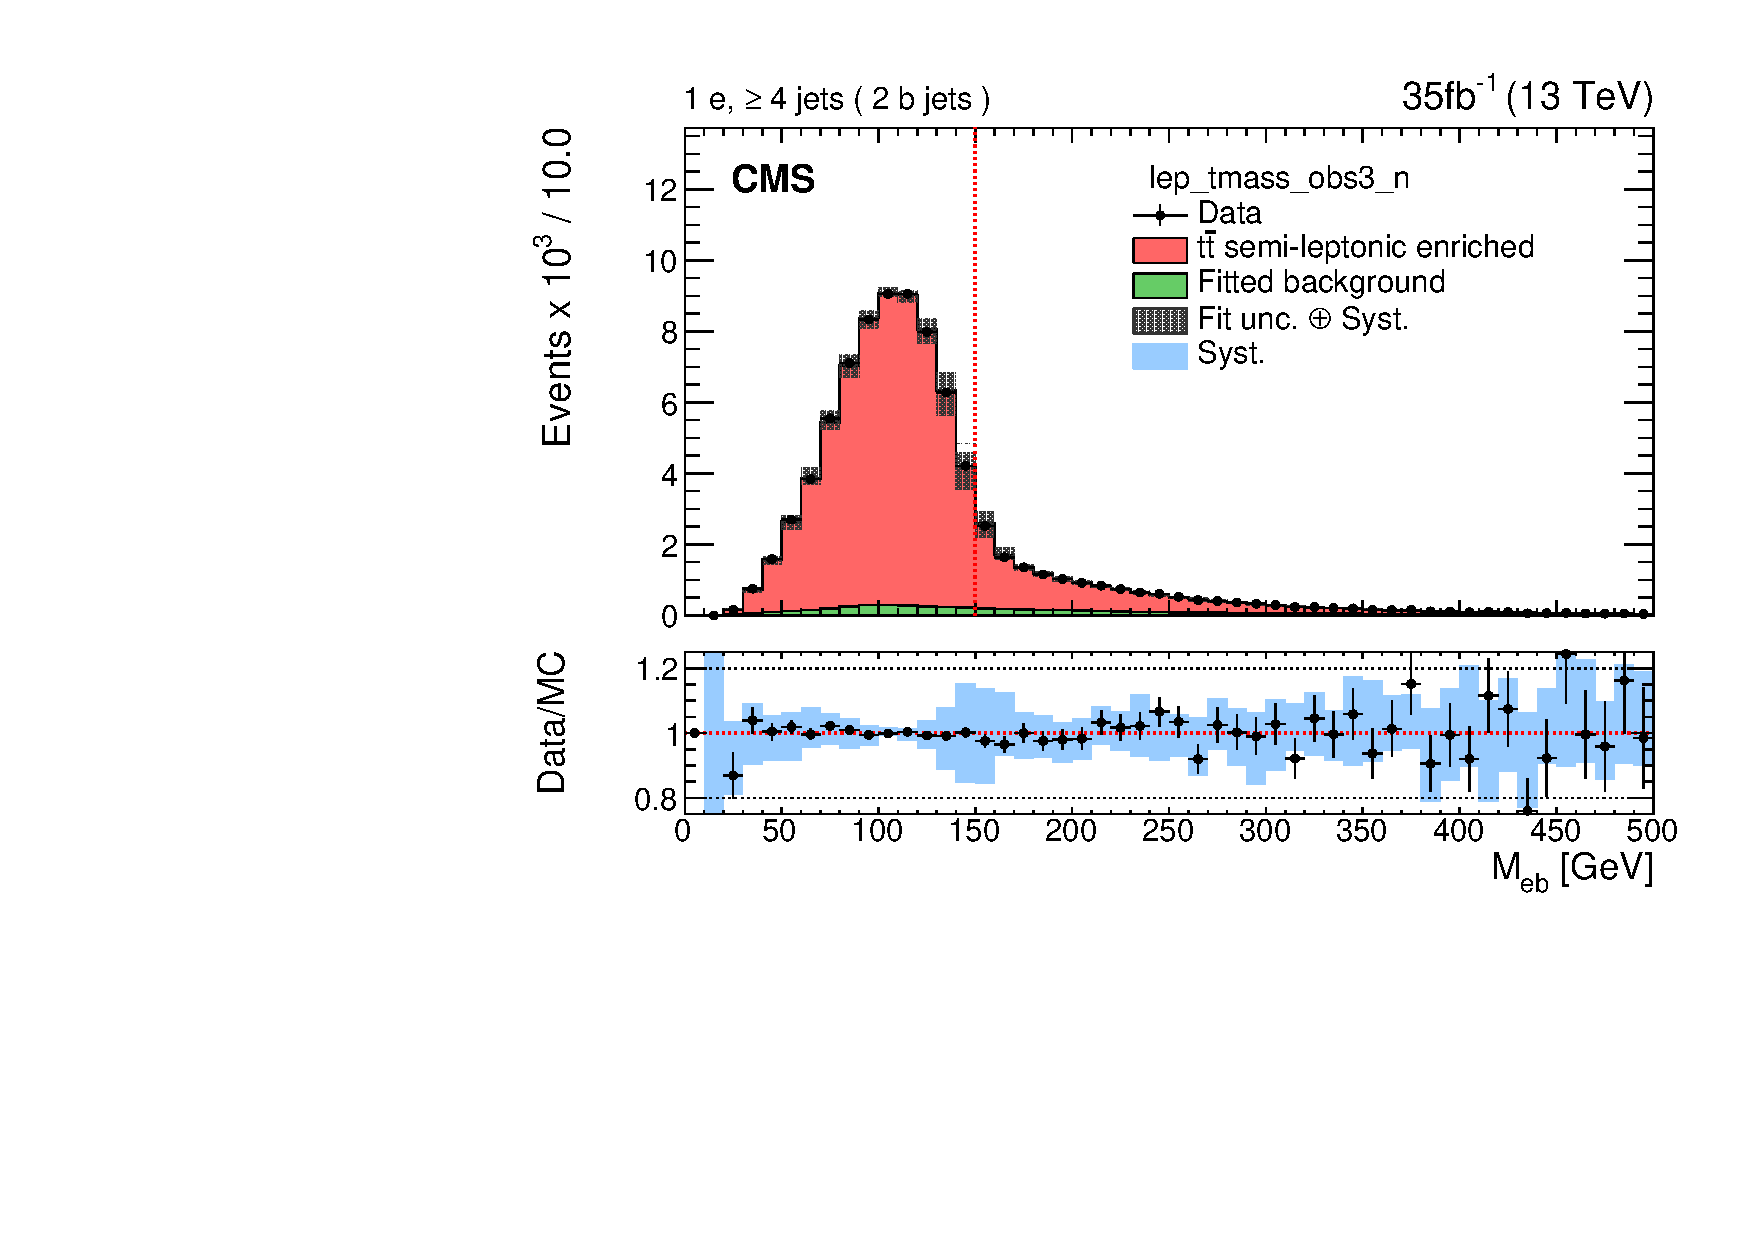
\includegraphics[width=0.4\textwidth]{figure/FitResult_16_el_lep_tmass_obs3_n_chi2_20.pdf}
    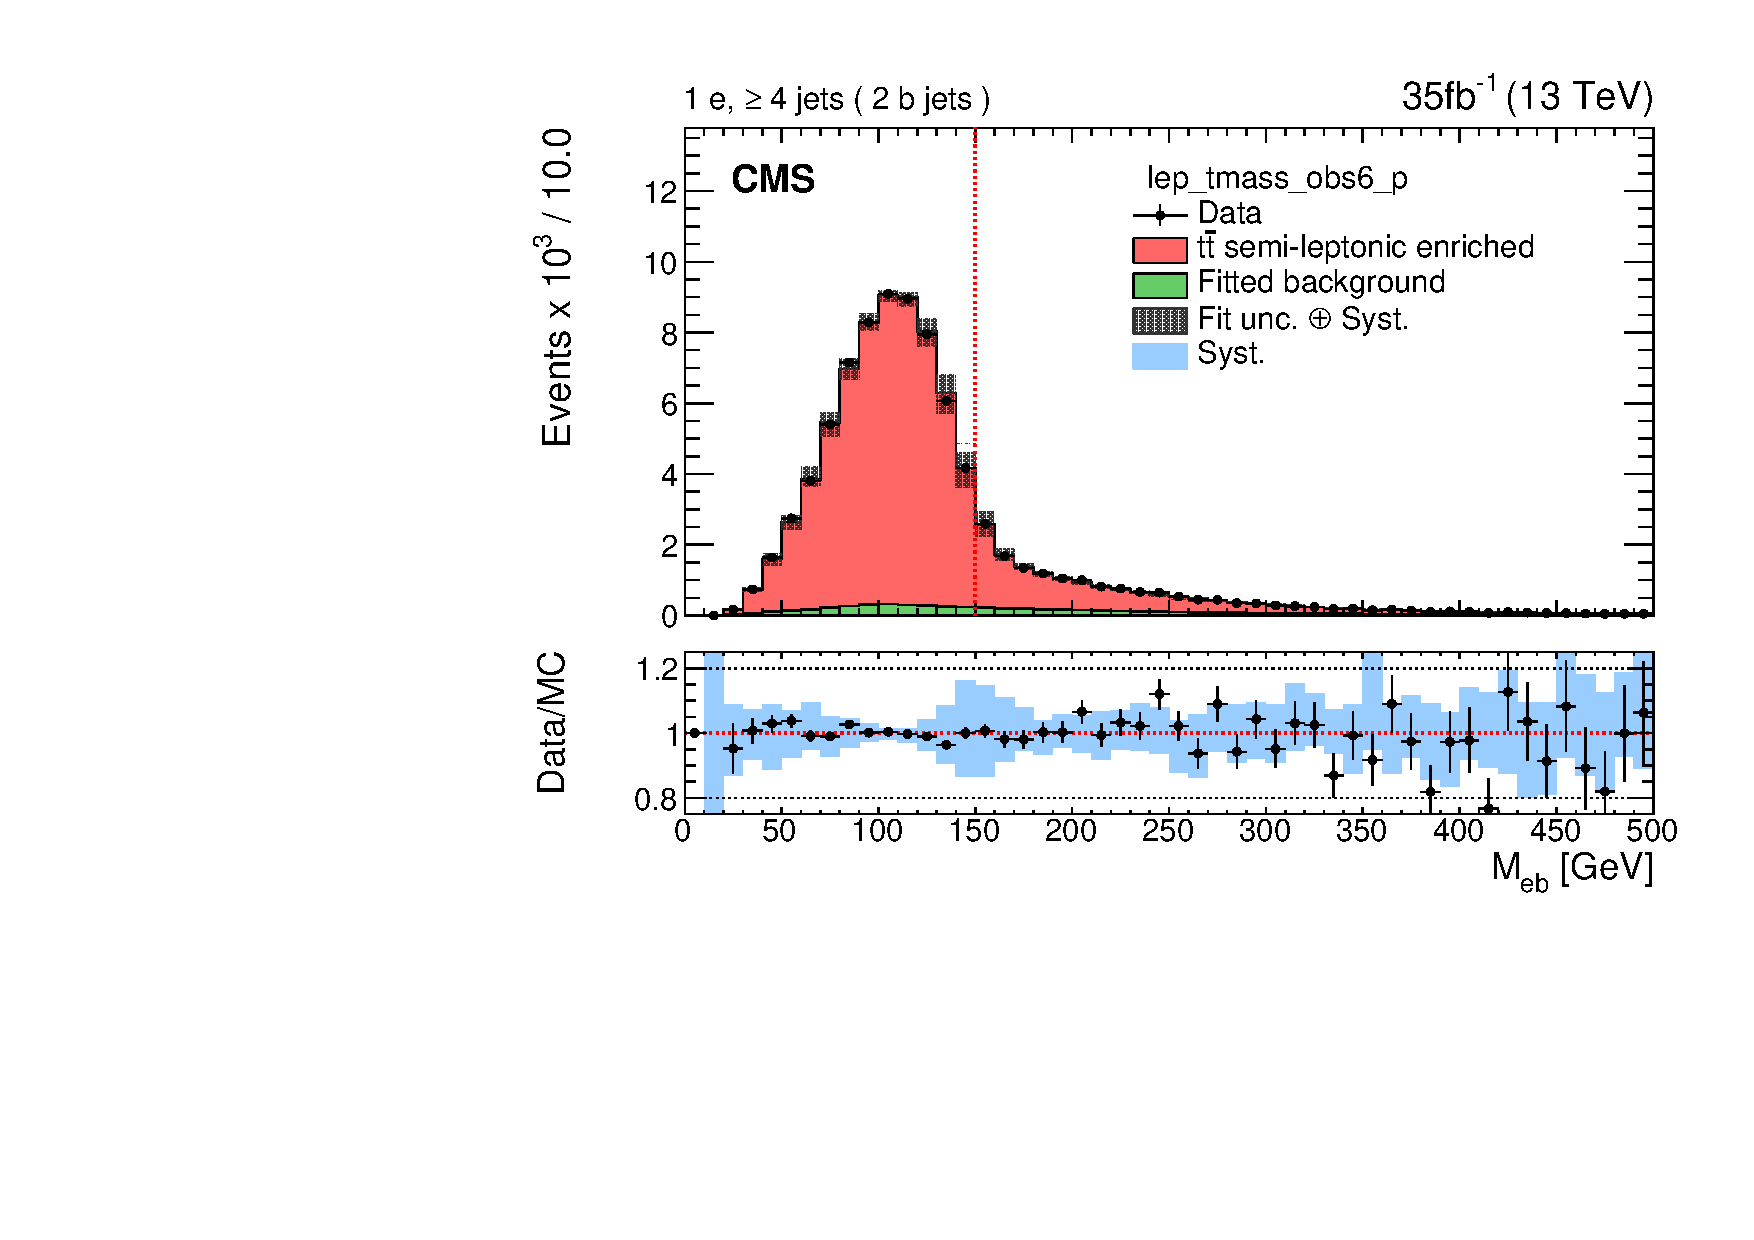
\includegraphics[width=0.4\textwidth]{figure/FitResult_16_el_lep_tmass_obs6_p_chi2_20.pdf}
    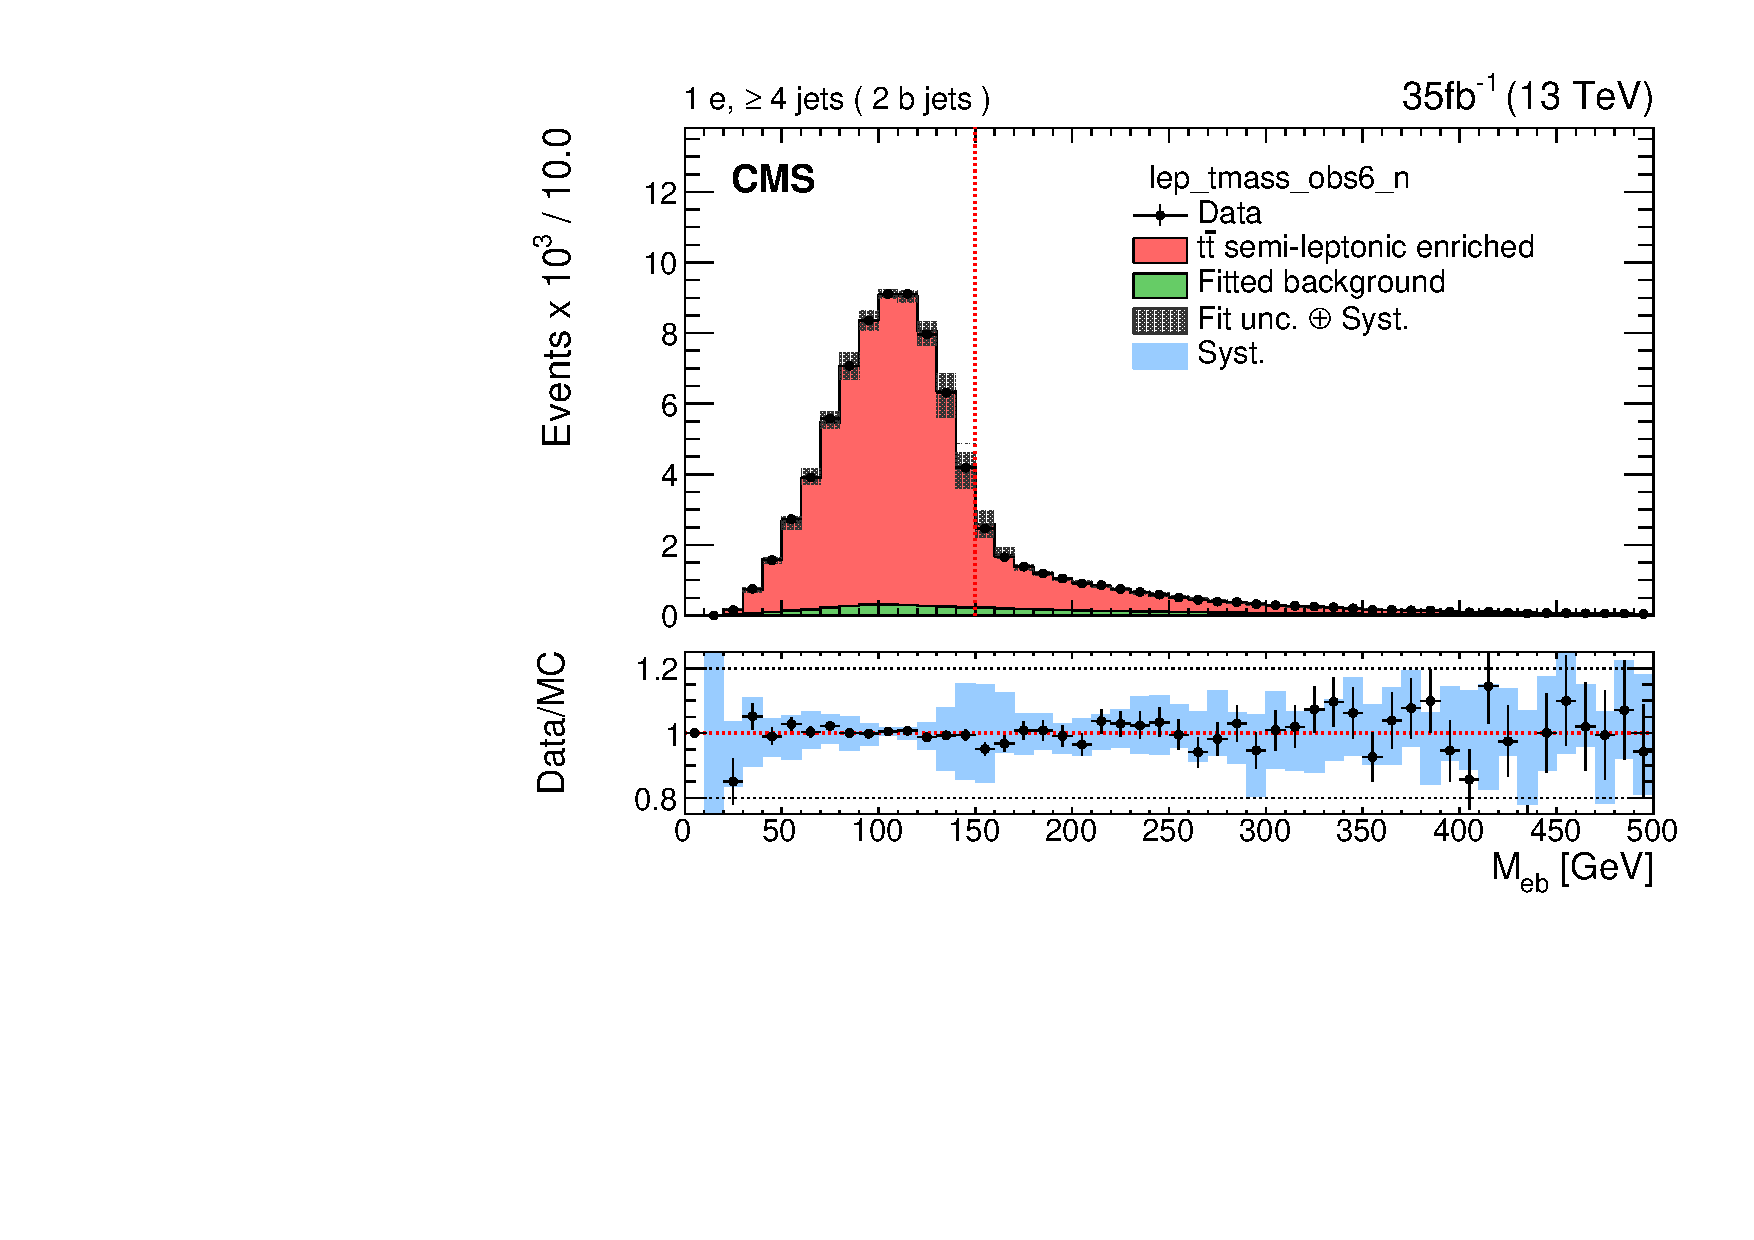
\includegraphics[width=0.4\textwidth]{figure/FitResult_16_el_lep_tmass_obs6_n_chi2_20.pdf}
    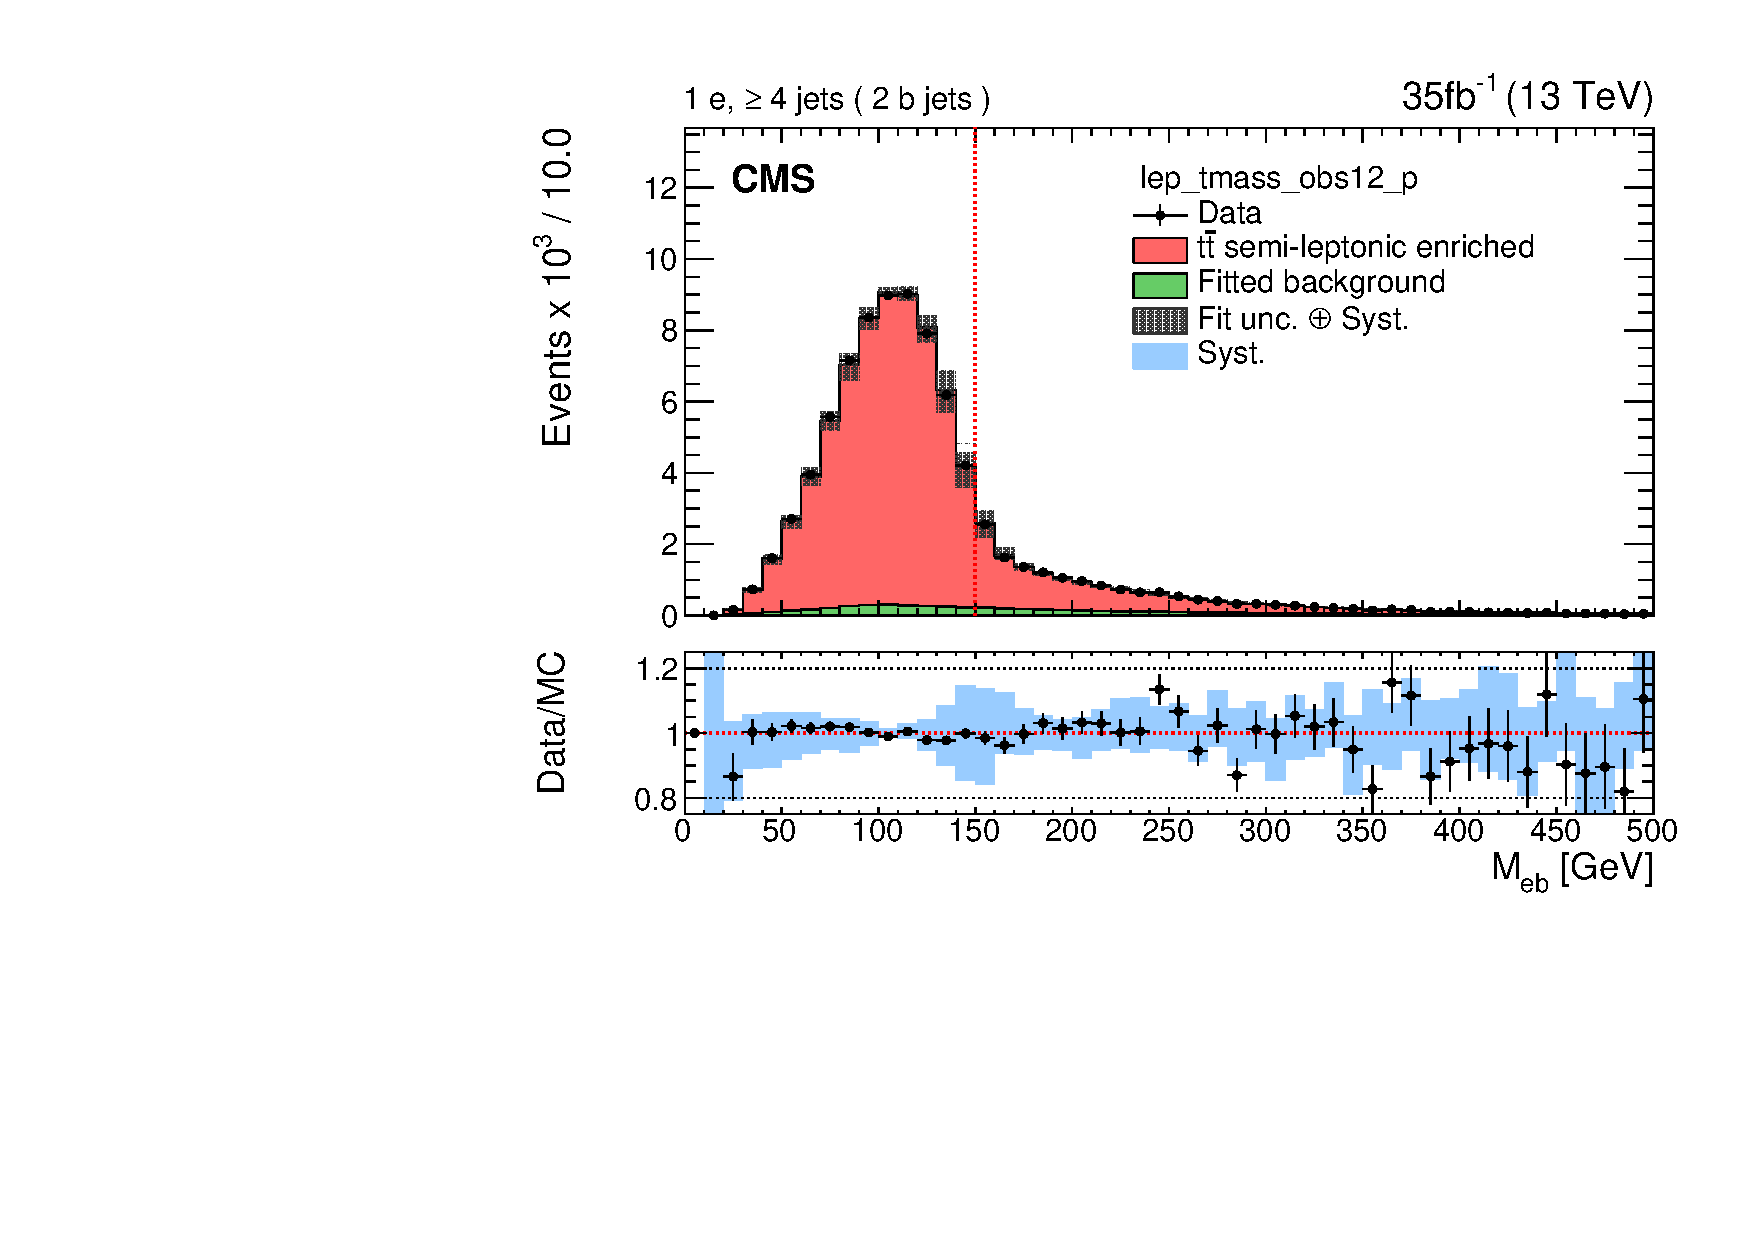
\includegraphics[width=0.4\textwidth]{figure/FitResult_16_el_lep_tmass_obs12_p_chi2_20.pdf}
    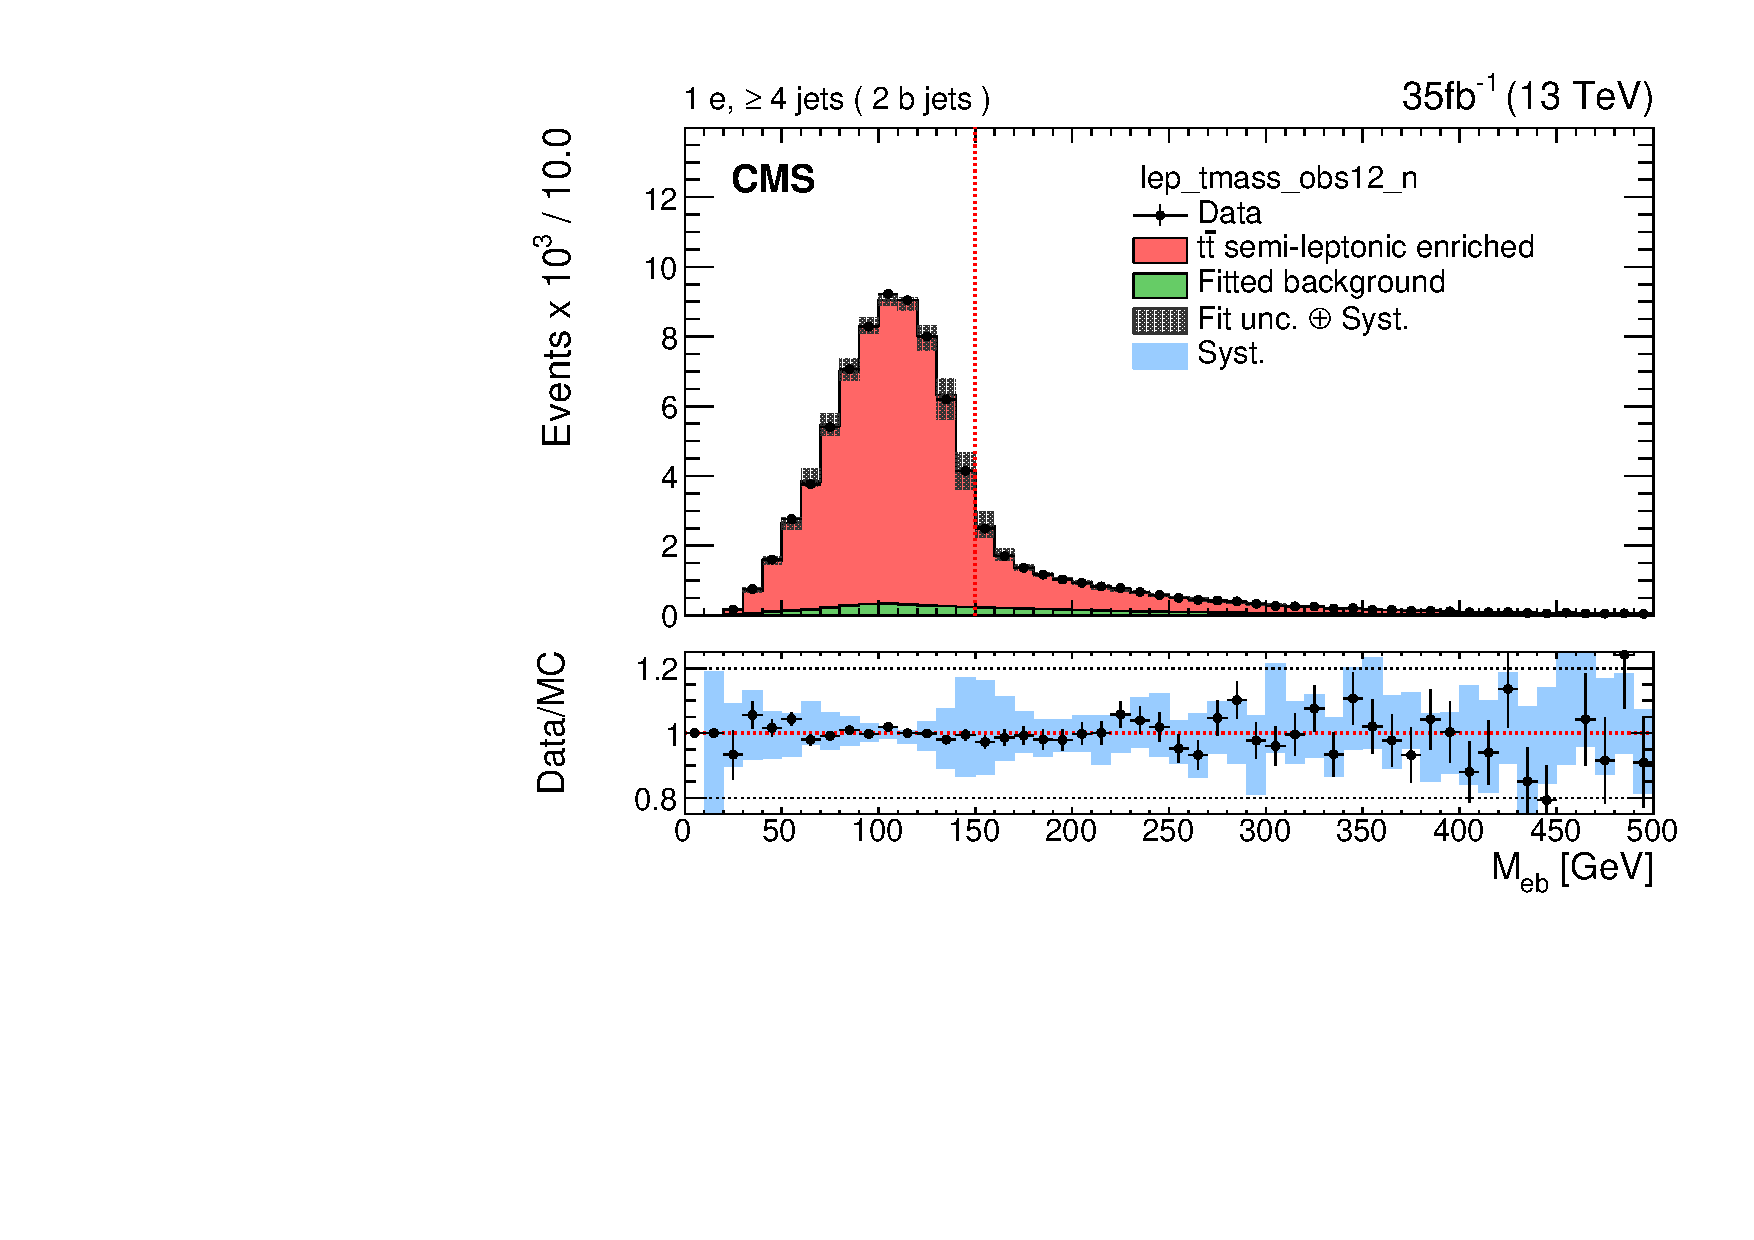
\includegraphics[width=0.4\textwidth]{figure/FitResult_16_el_lep_tmass_obs12_n_chi2_20.pdf}
    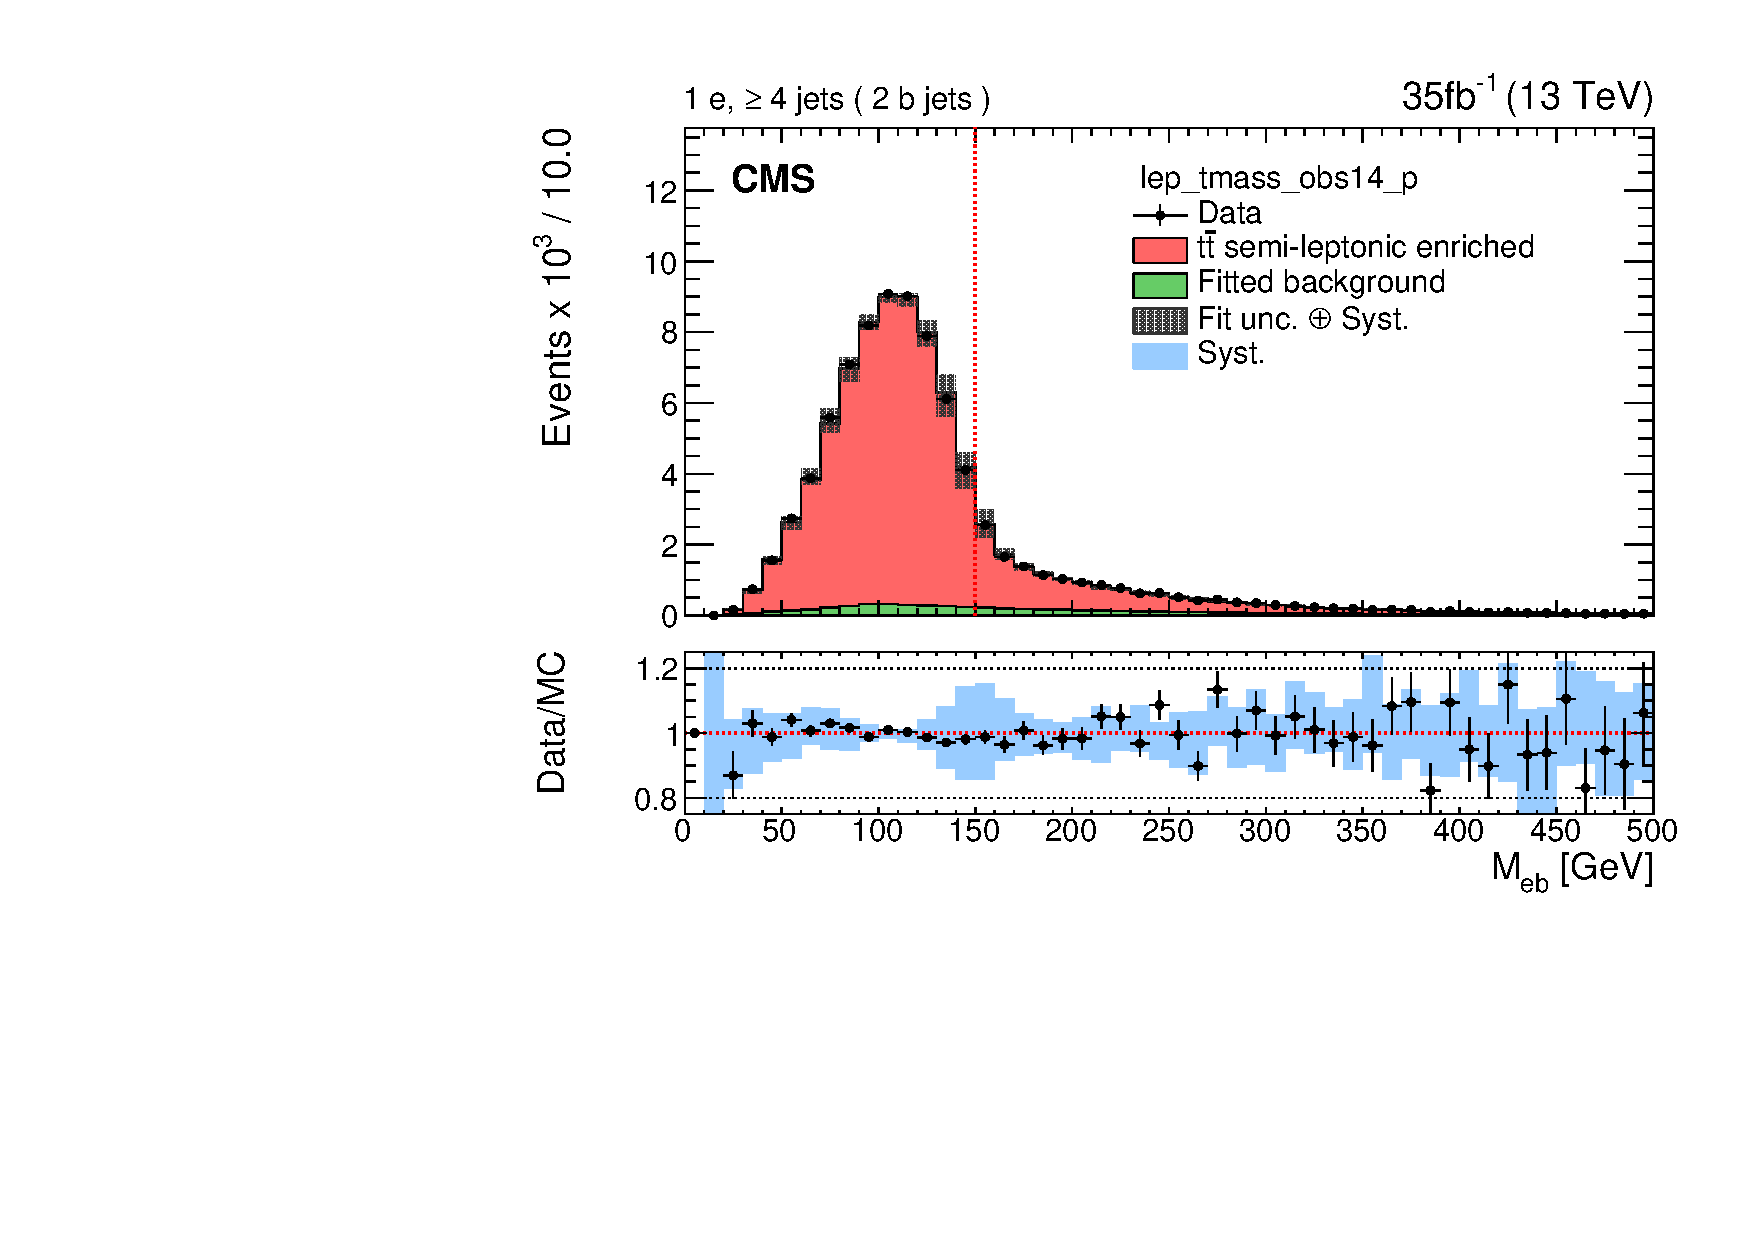
\includegraphics[width=0.4\textwidth]{figure/FitResult_16_el_lep_tmass_obs14_p_chi2_20.pdf}
    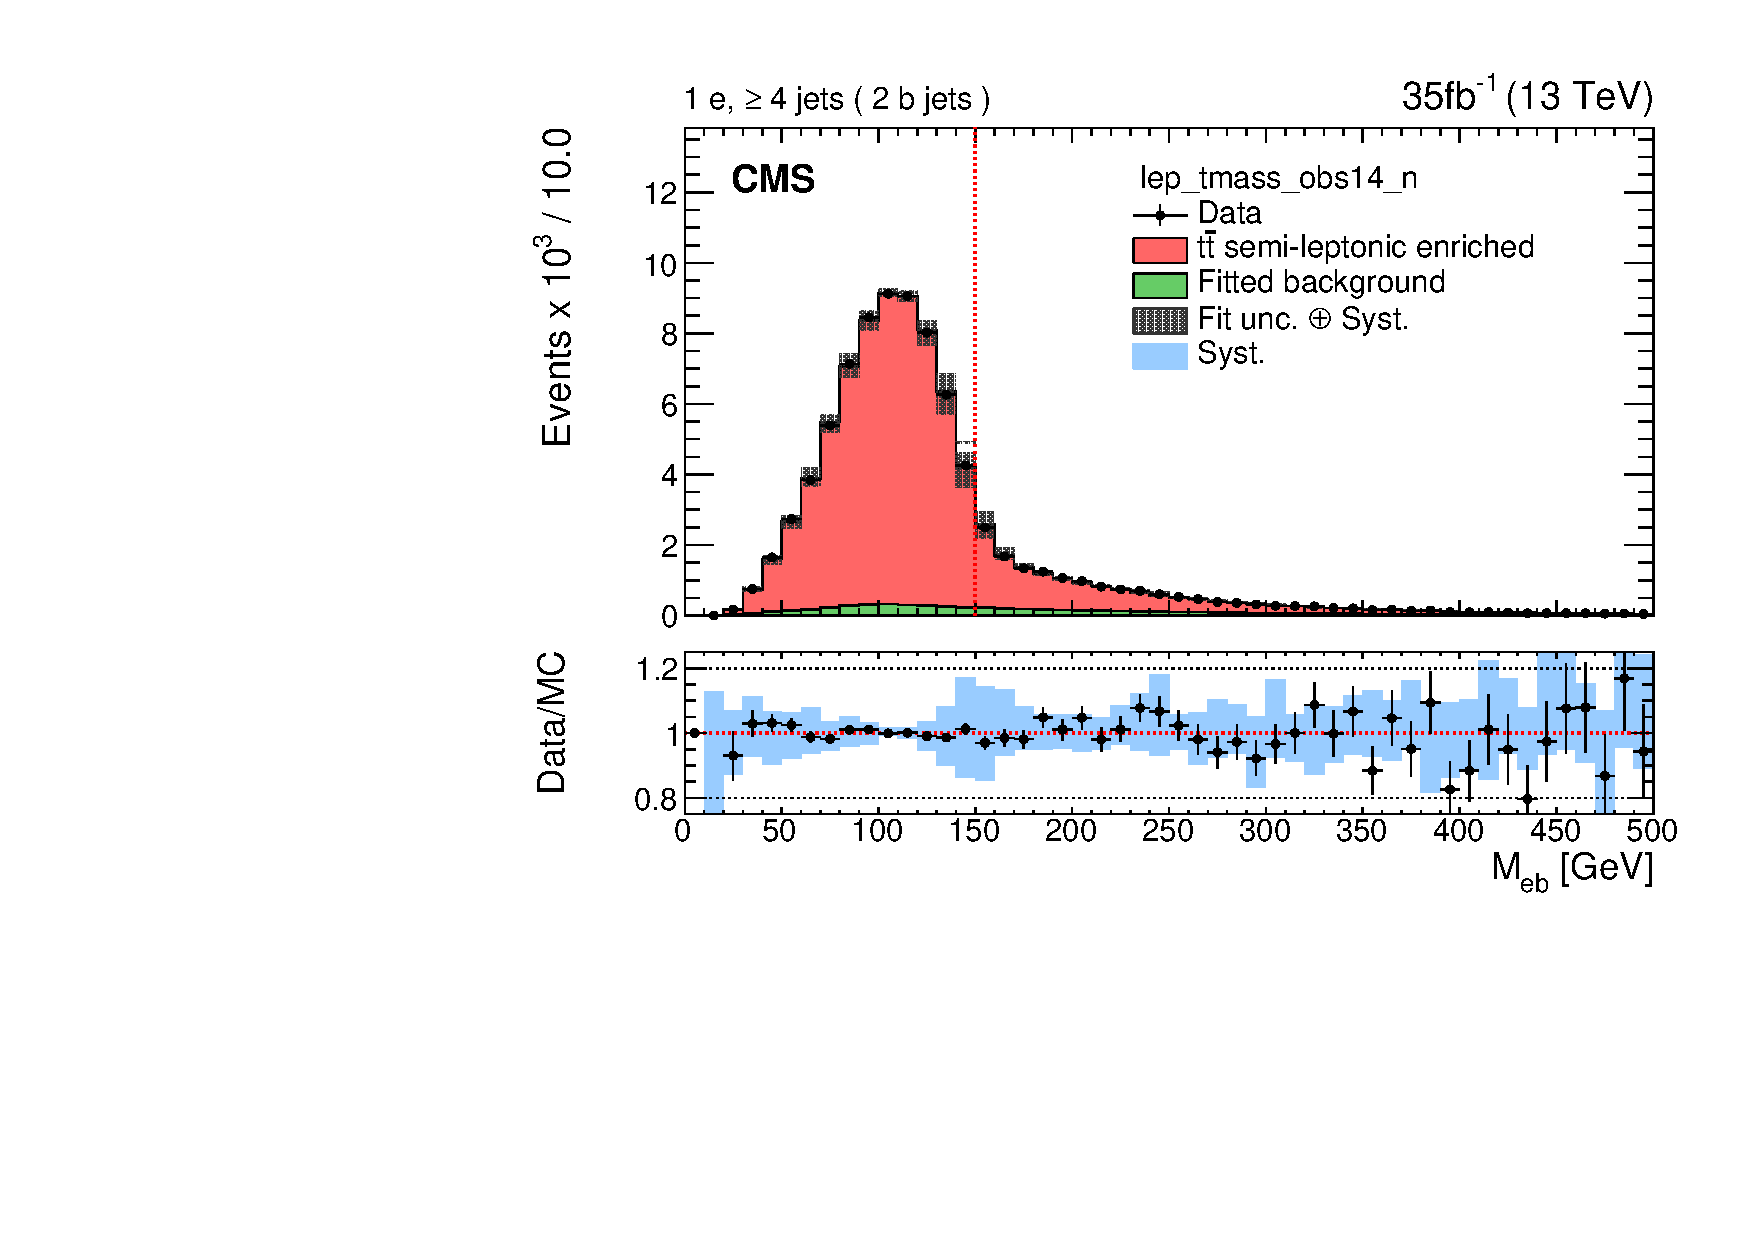
\includegraphics[width=0.4\textwidth]{figure/FitResult_16_el_lep_tmass_obs14_n_chi2_20.pdf}
    \caption[The \Mlb invariant mass distributions in electron channel from 2016 data.]
    {
        The \Mlb invariant mass distributions in the positive (left) and negative (right) observable value region in electron channel from 2016 data (points).
        The results of the fit to the \ttbar and background templates are shown by the red and green histograms, respectively.
        The vertical bars on the data points in the upper panels indicate the statistical uncertainties in the data and the hatched bands show the combined statistical and systematic uncertainties in the simulation.
        The lower panels give the ratio of the data to the sum of the fitted MC predictions.
        The blue bands represent the systematic uncertainties in the expected yield in the simulation for all sources of systematic uncertainty (Section~\ref{sec:uncertainty}).
    }
    \label{fig:fitting_results_16_el}
\end{figure}

\begin{figure}
    \centering
    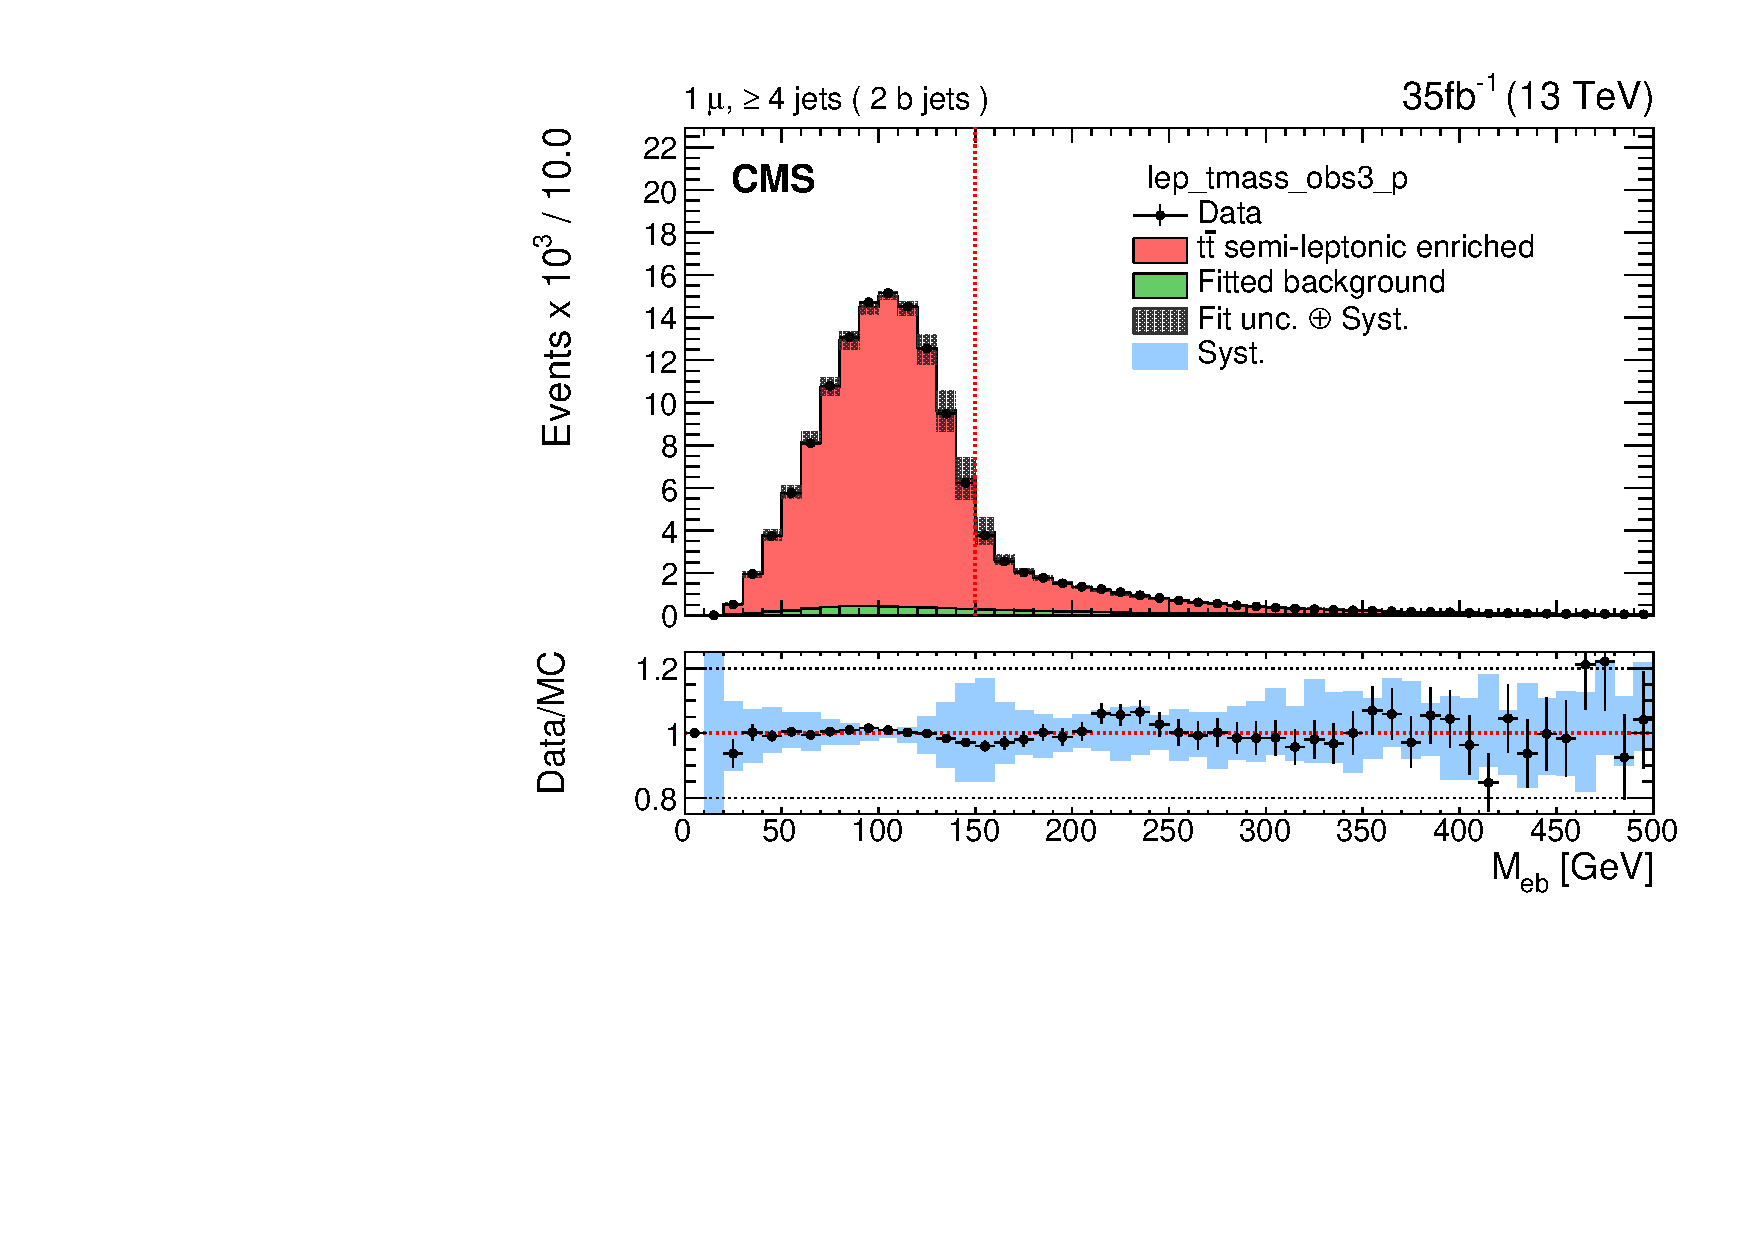
\includegraphics[width=0.4\textwidth]{figure/FitResult_16_mu_lep_tmass_obs3_p_chi2_20.pdf}
    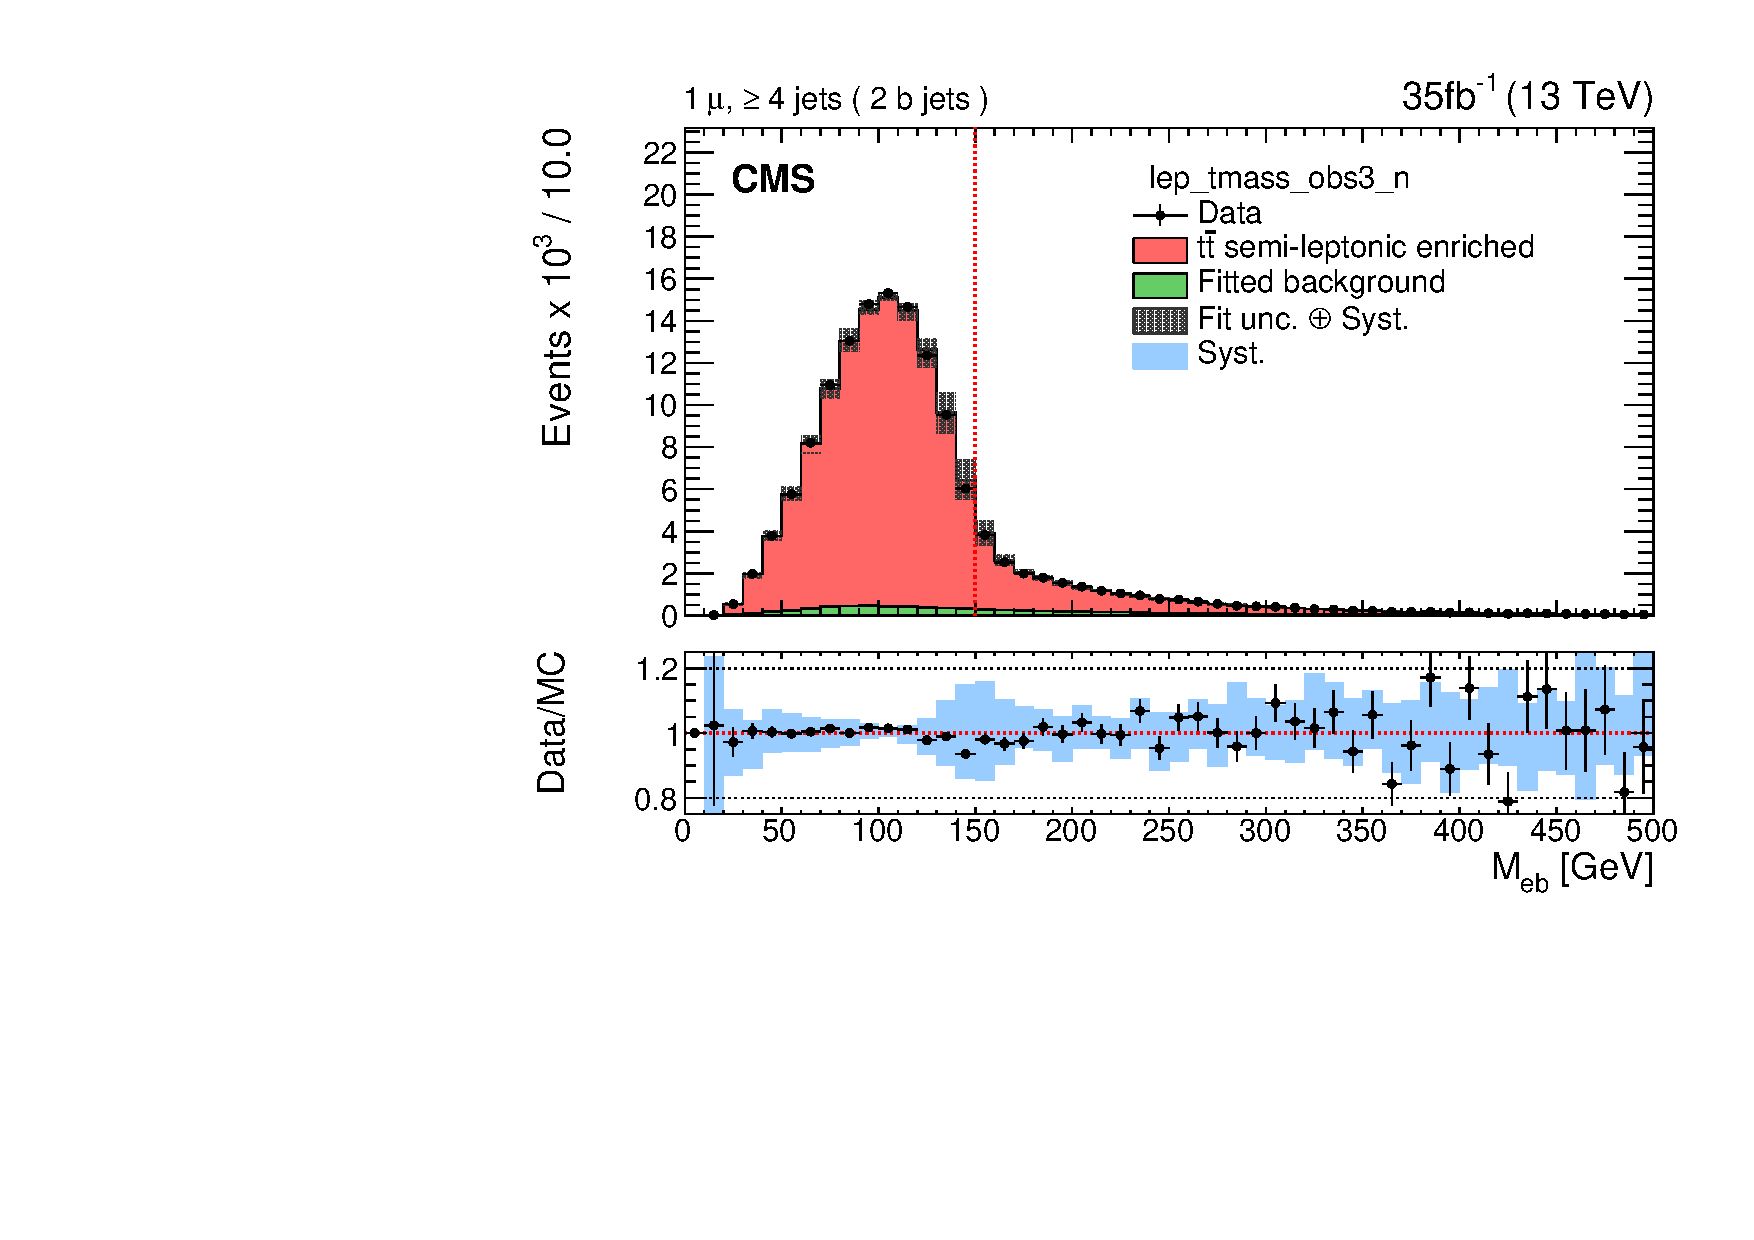
\includegraphics[width=0.4\textwidth]{figure/FitResult_16_mu_lep_tmass_obs3_n_chi2_20.pdf}
    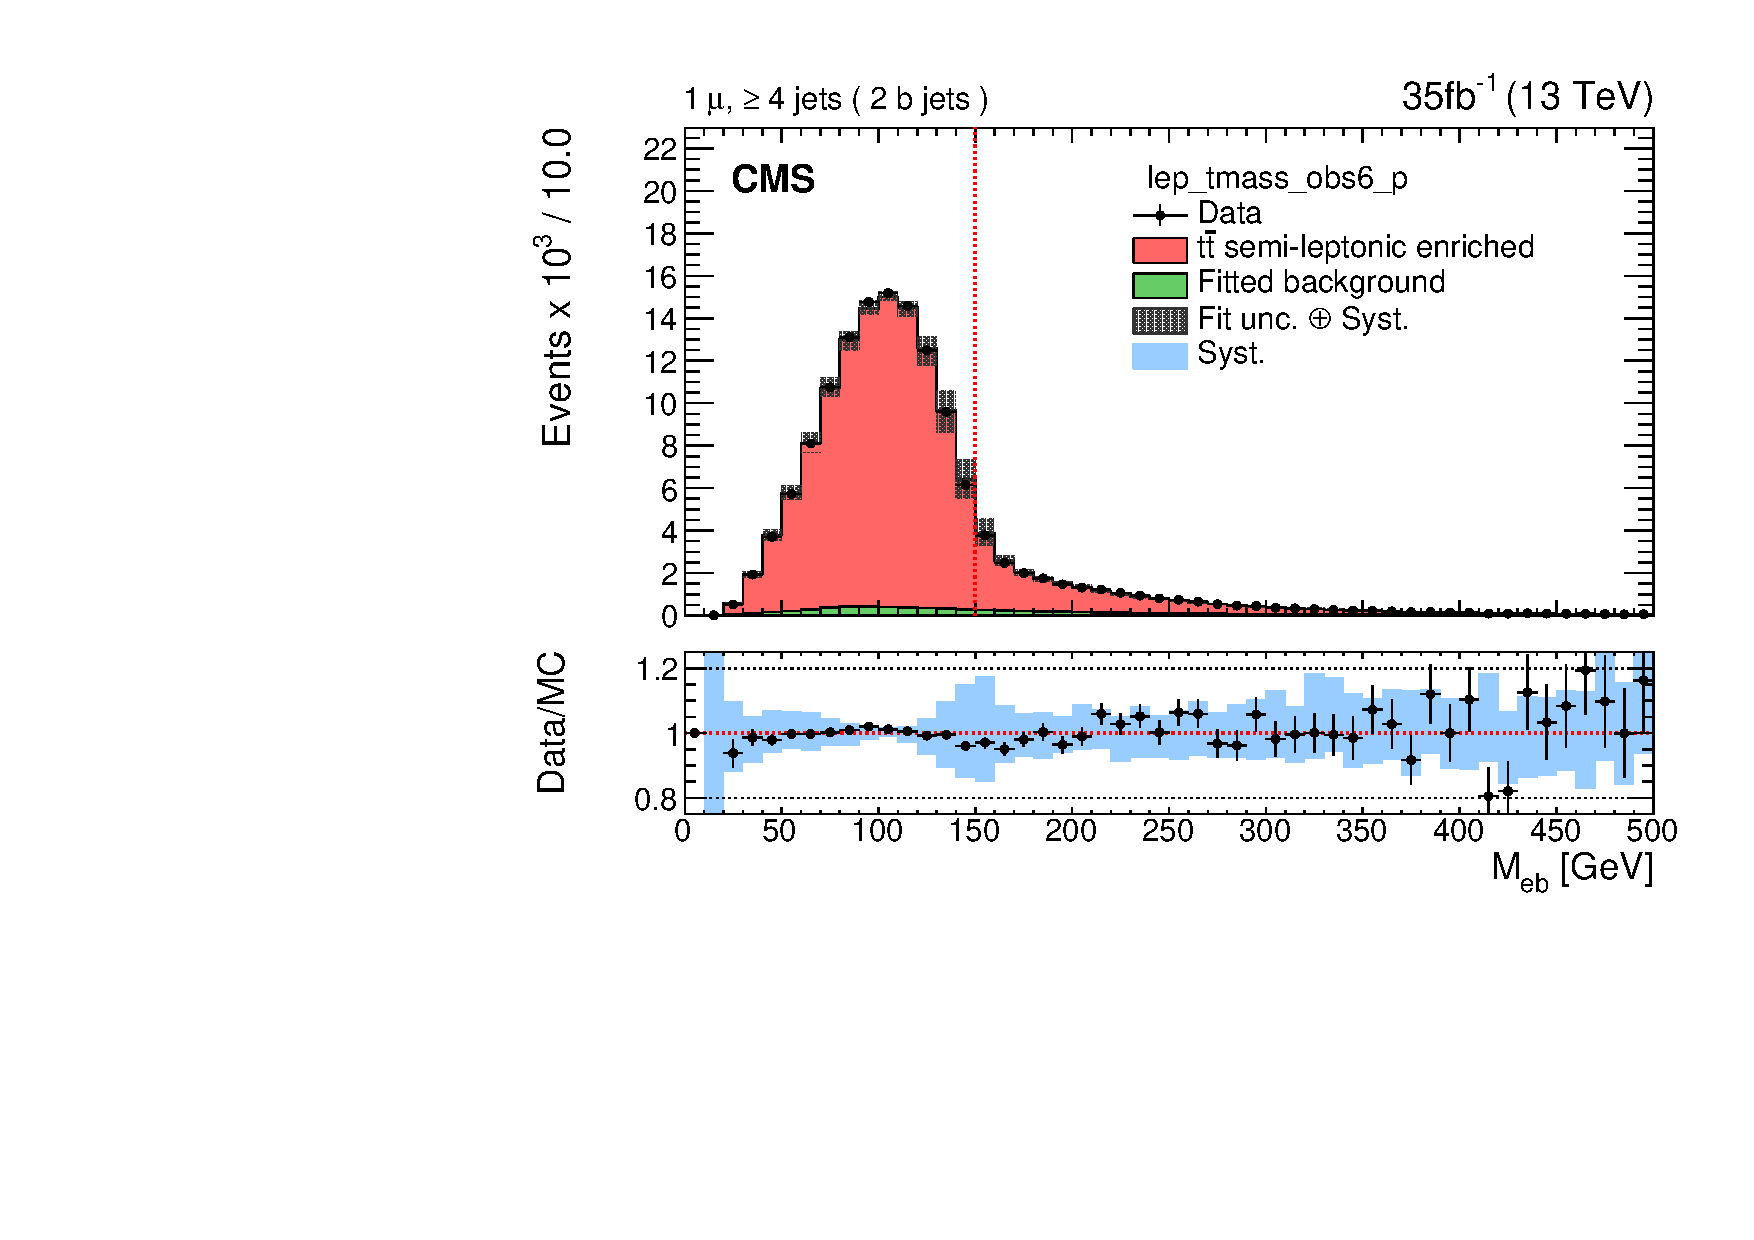
\includegraphics[width=0.4\textwidth]{figure/FitResult_16_mu_lep_tmass_obs6_p_chi2_20.pdf}
    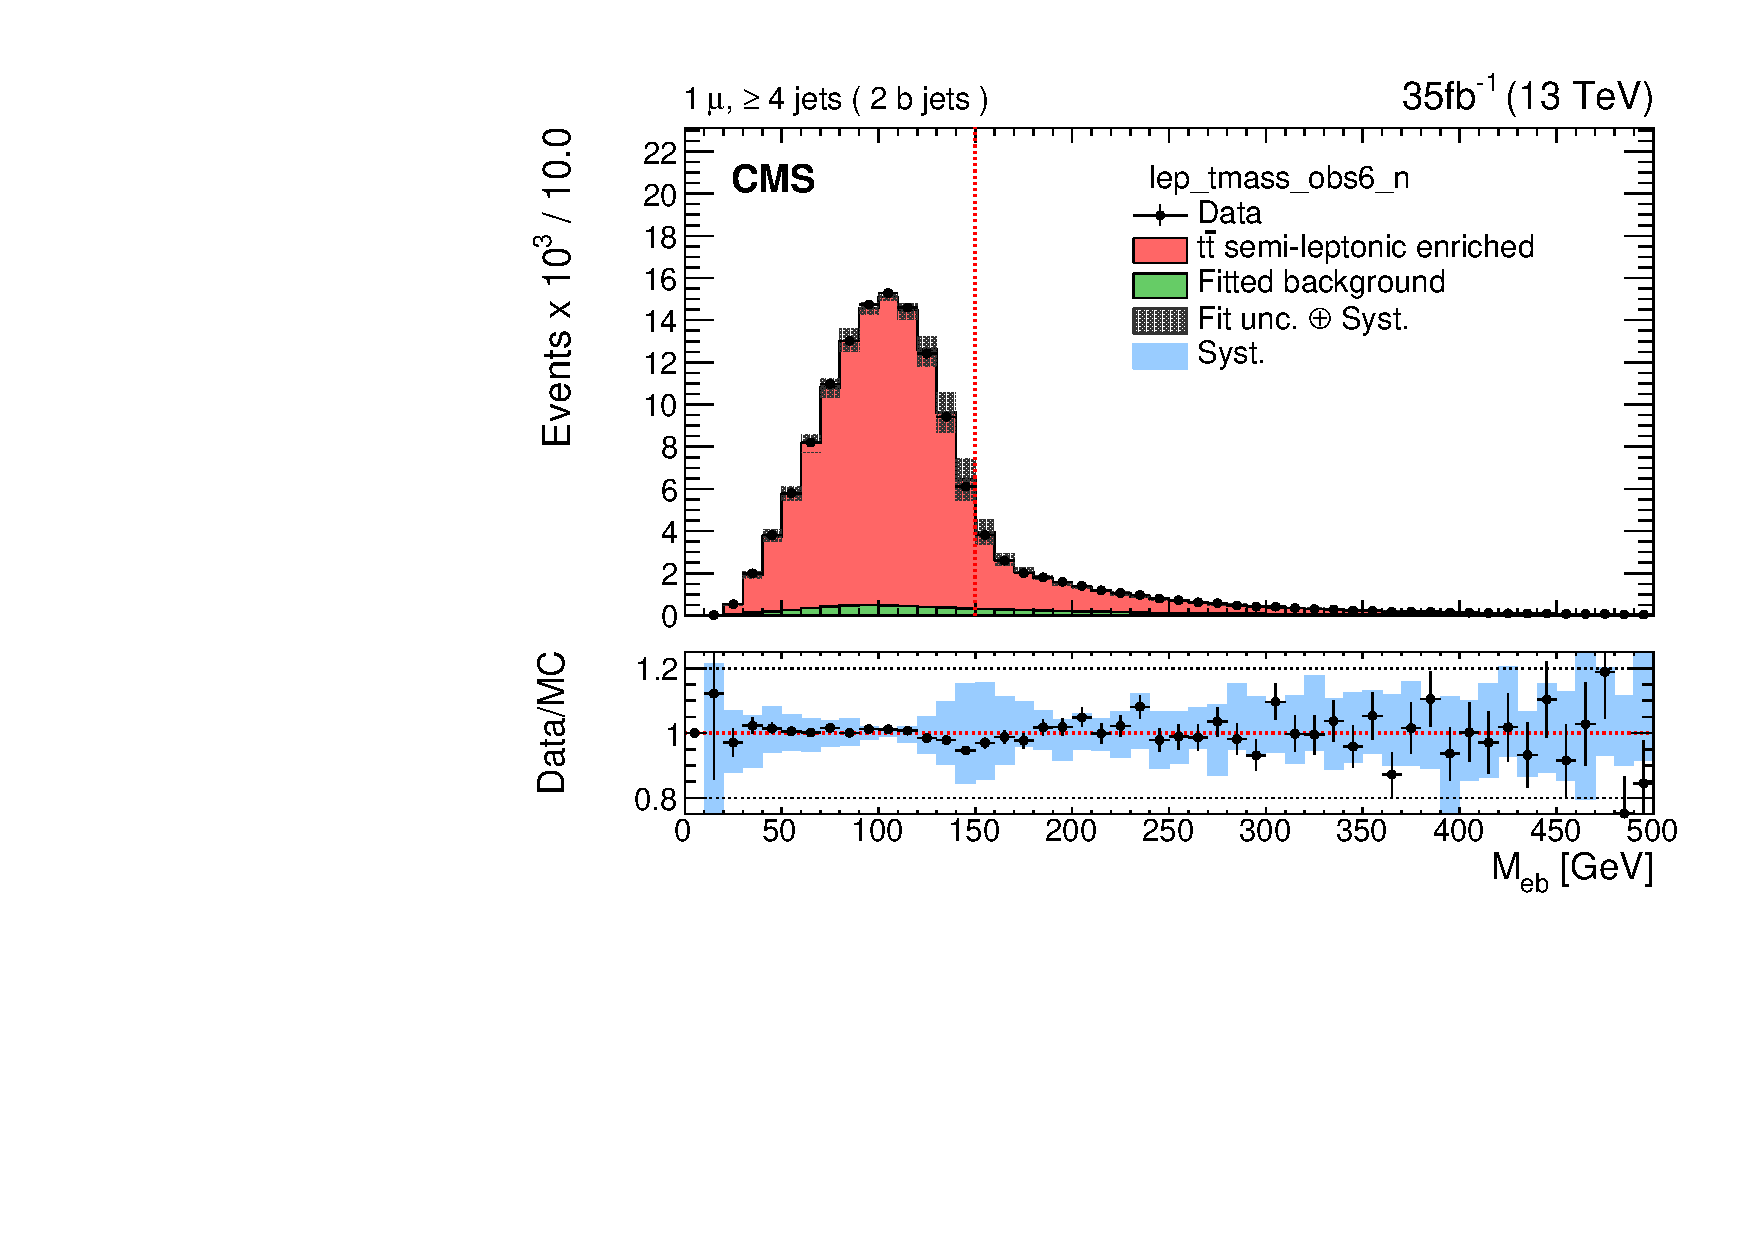
\includegraphics[width=0.4\textwidth]{figure/FitResult_16_mu_lep_tmass_obs6_n_chi2_20.pdf}
    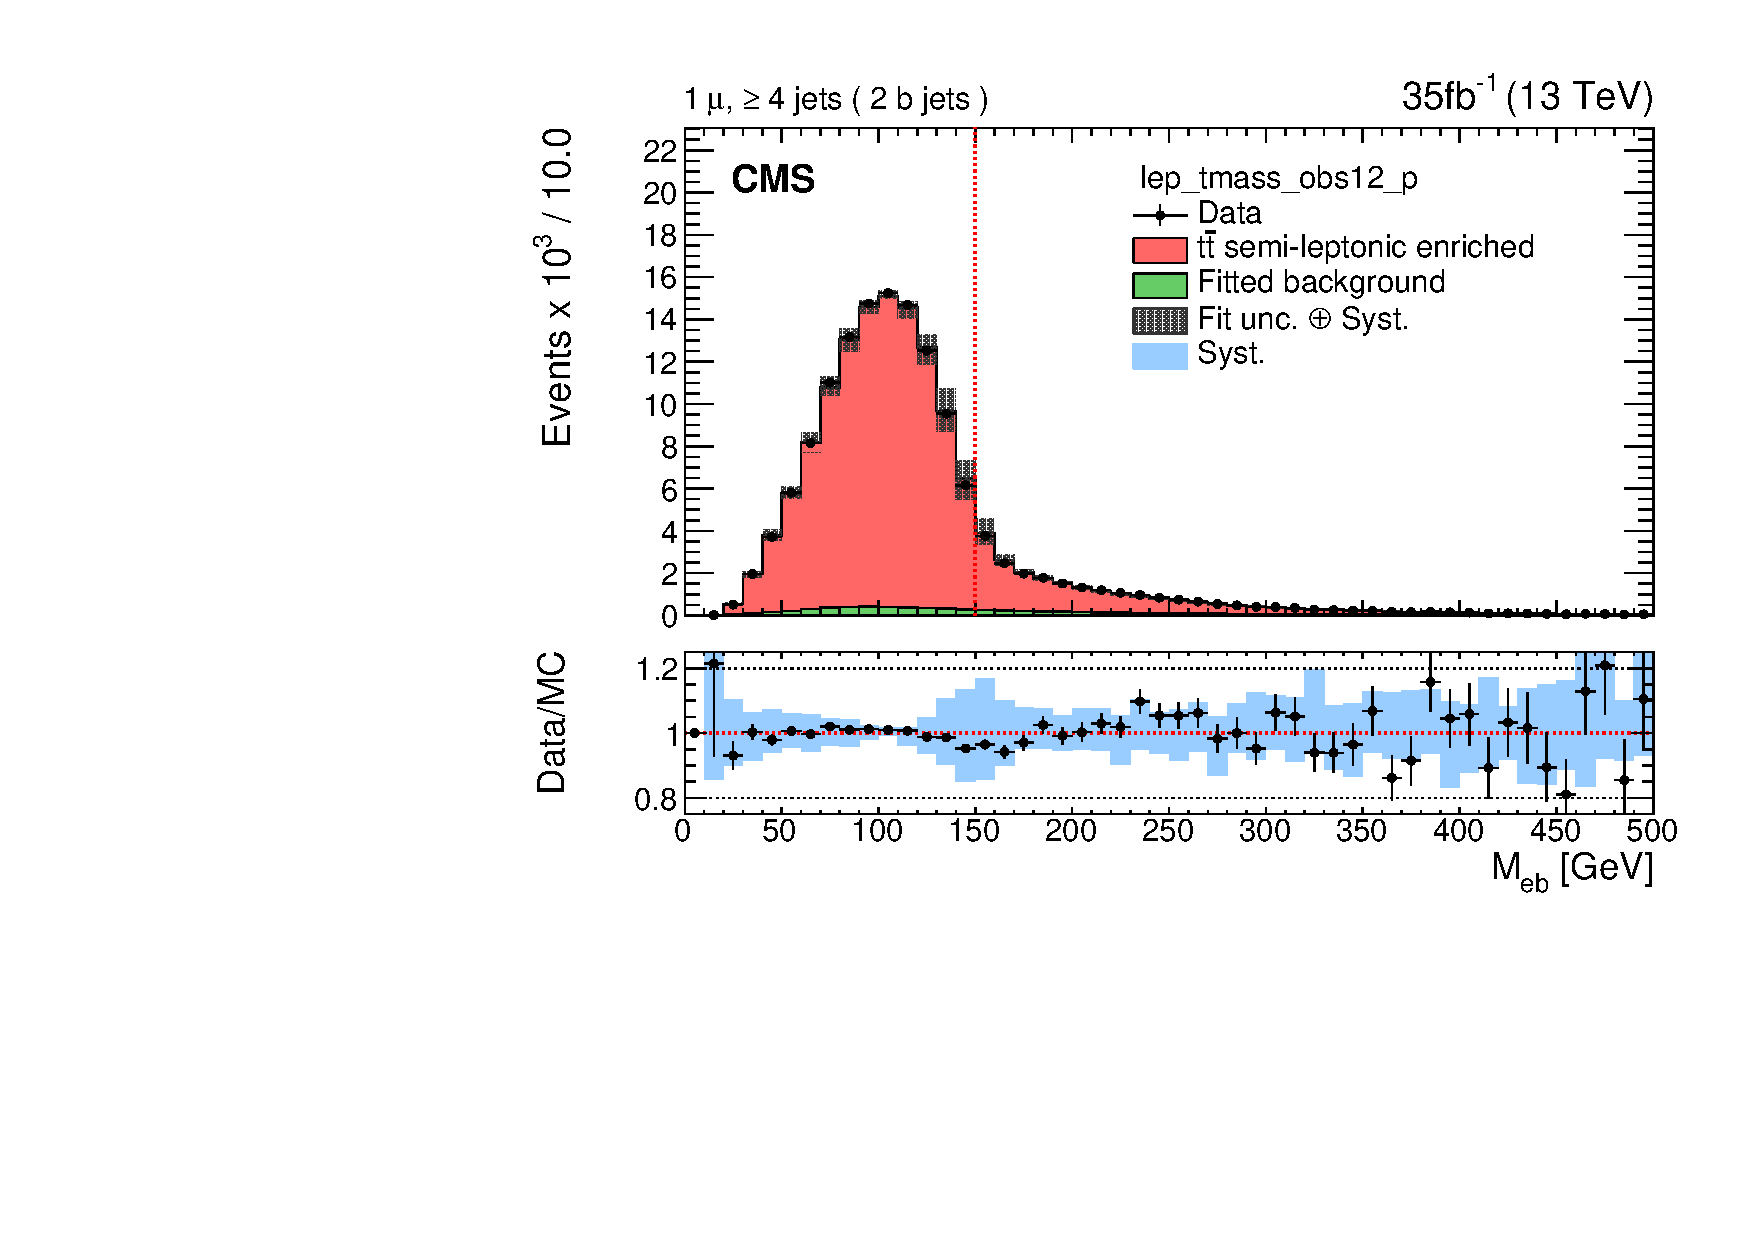
\includegraphics[width=0.4\textwidth]{figure/FitResult_16_mu_lep_tmass_obs12_p_chi2_20.pdf}
    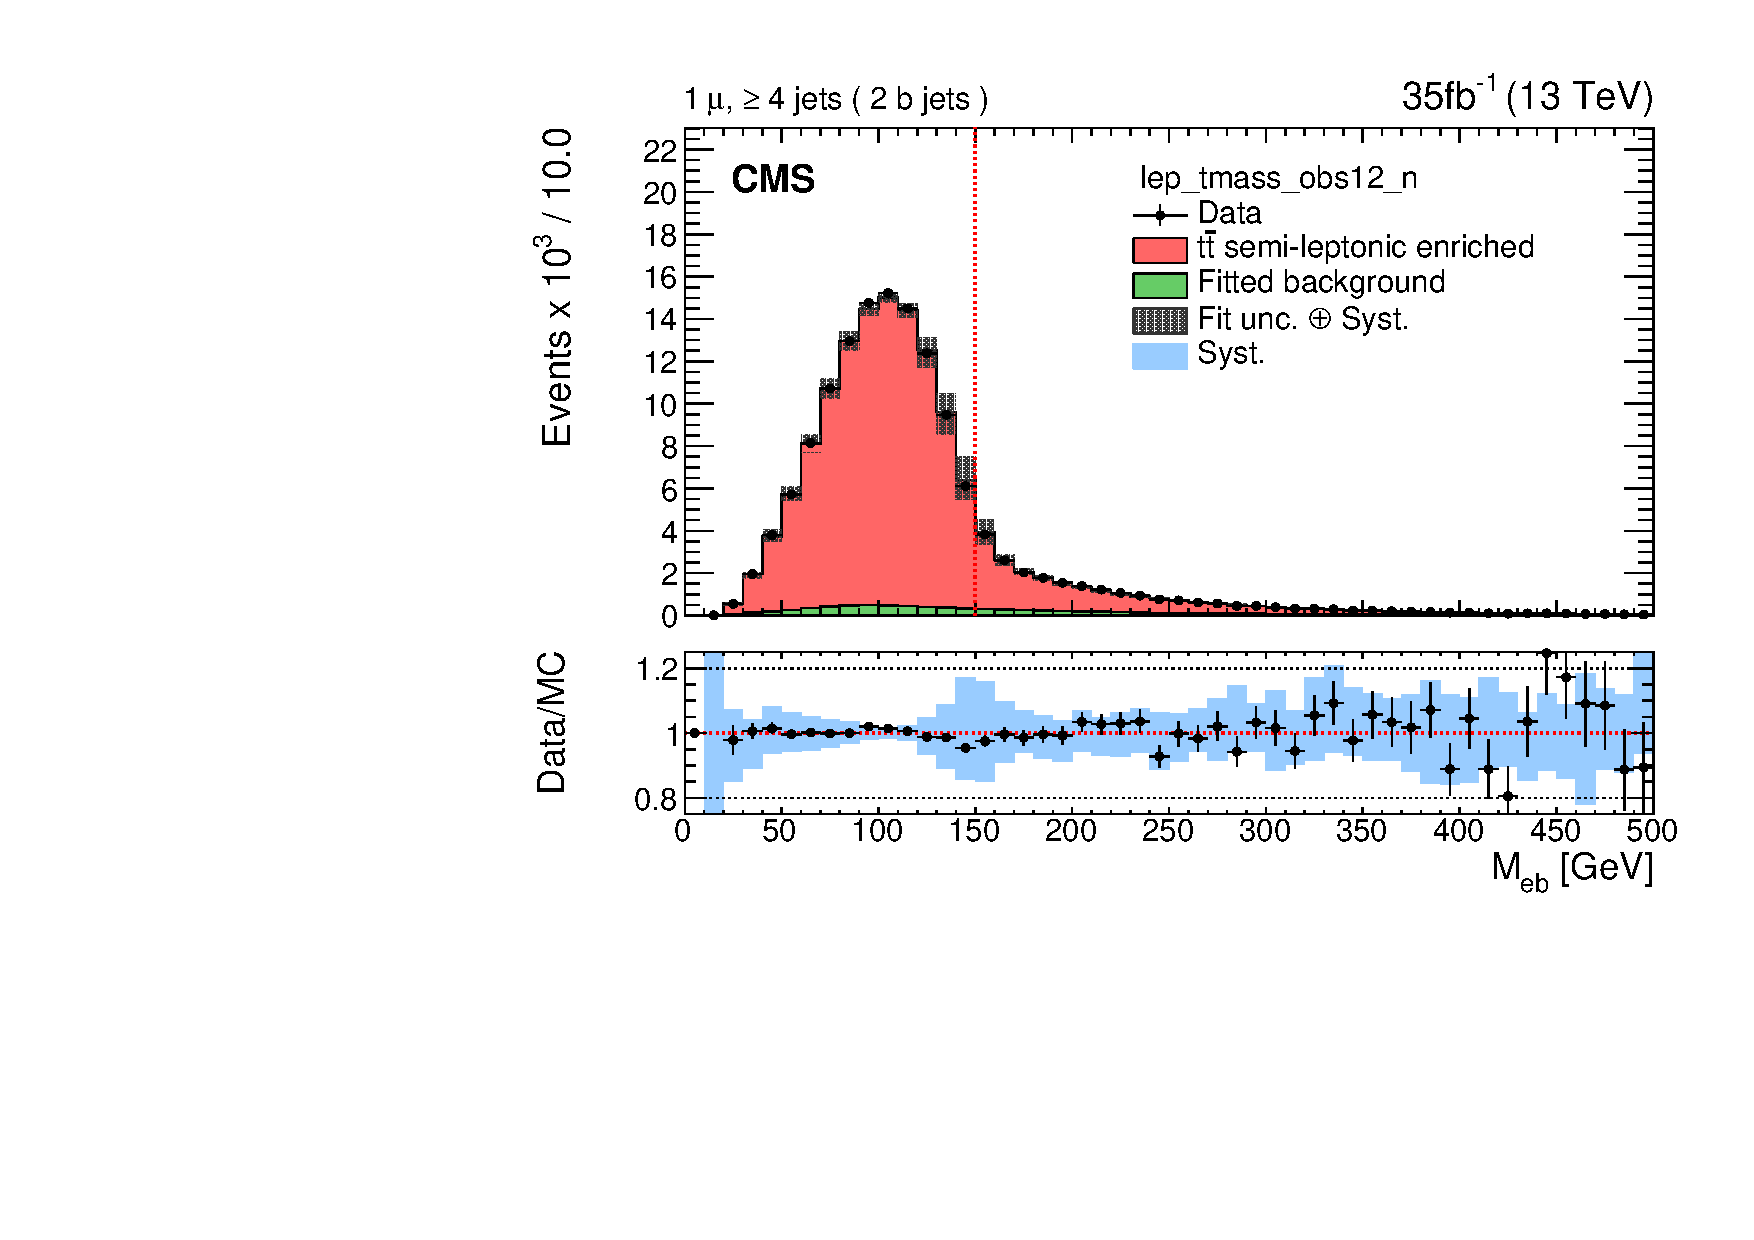
\includegraphics[width=0.4\textwidth]{figure/FitResult_16_mu_lep_tmass_obs12_n_chi2_20.pdf}
    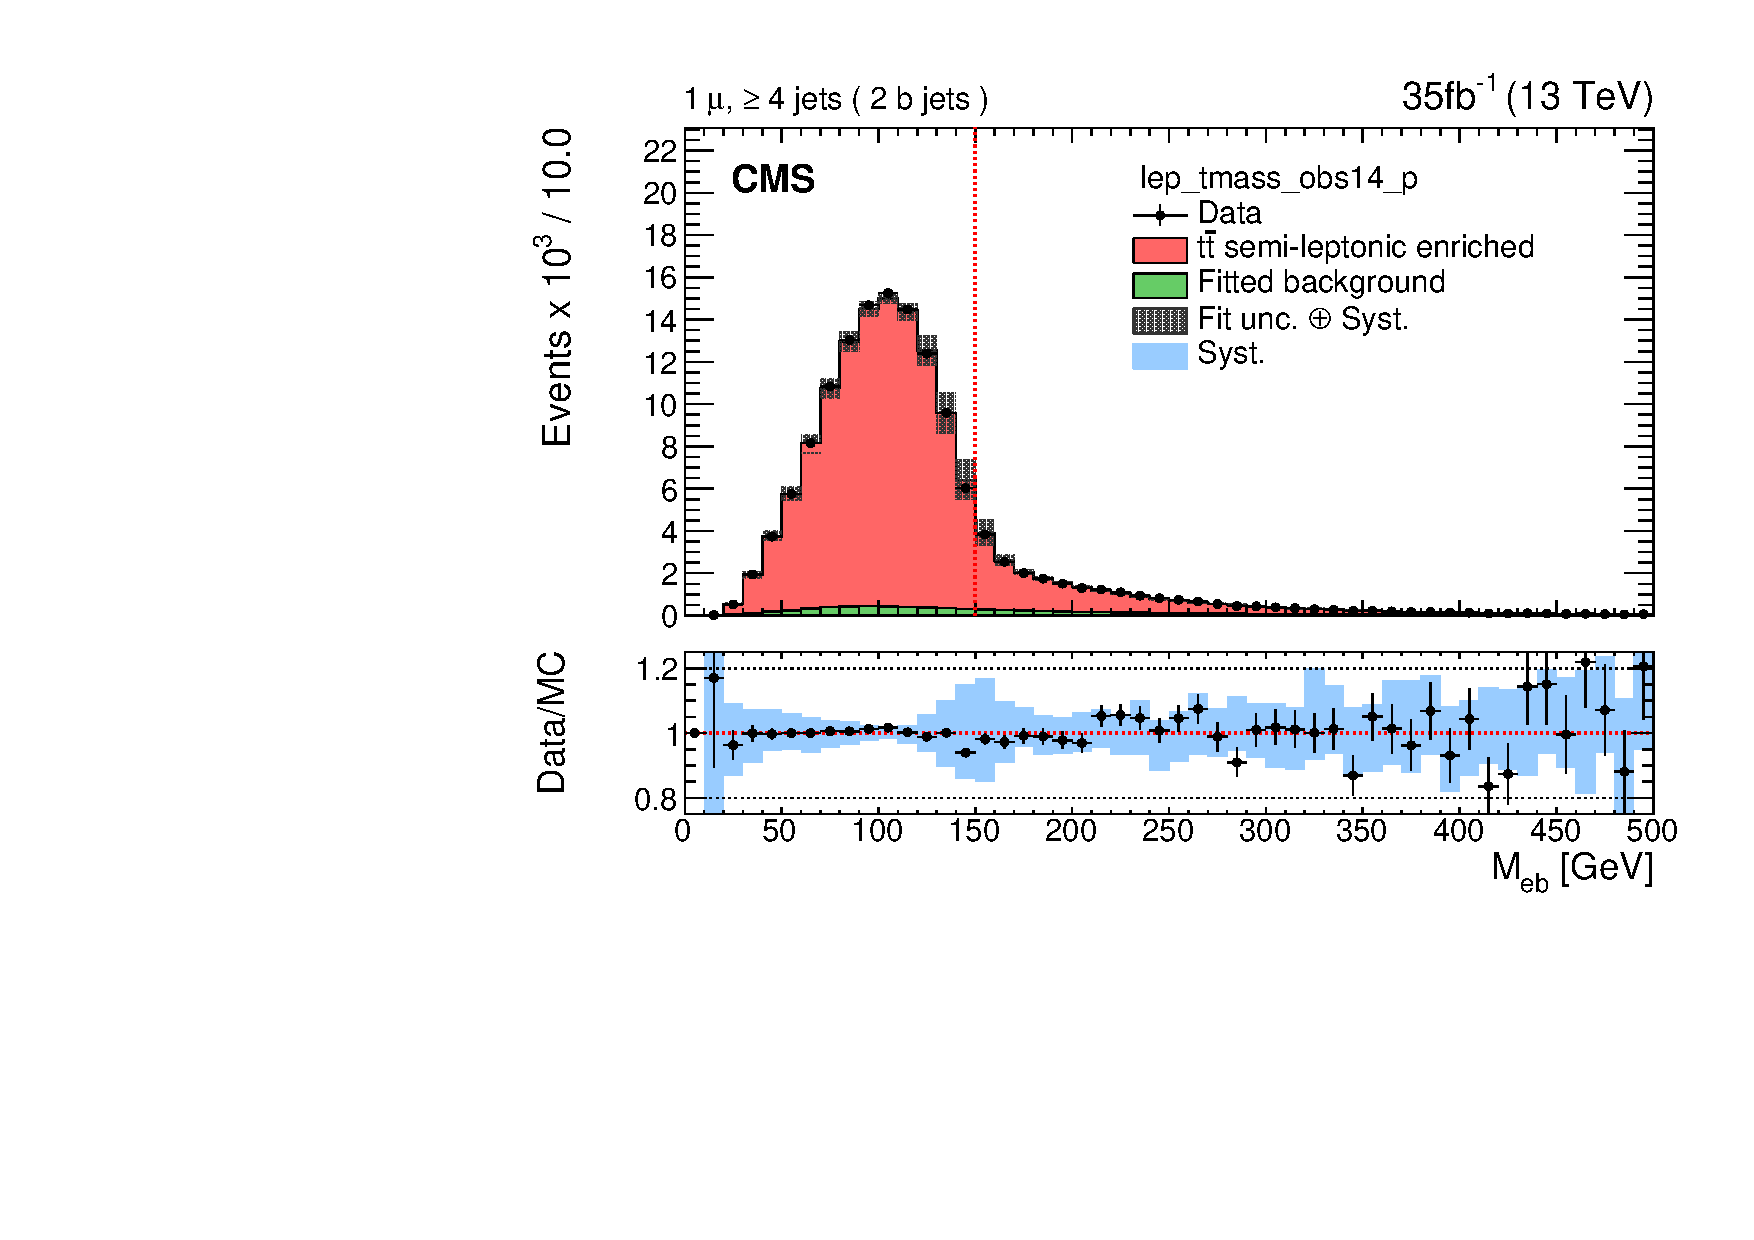
\includegraphics[width=0.4\textwidth]{figure/FitResult_16_mu_lep_tmass_obs14_p_chi2_20.pdf}
    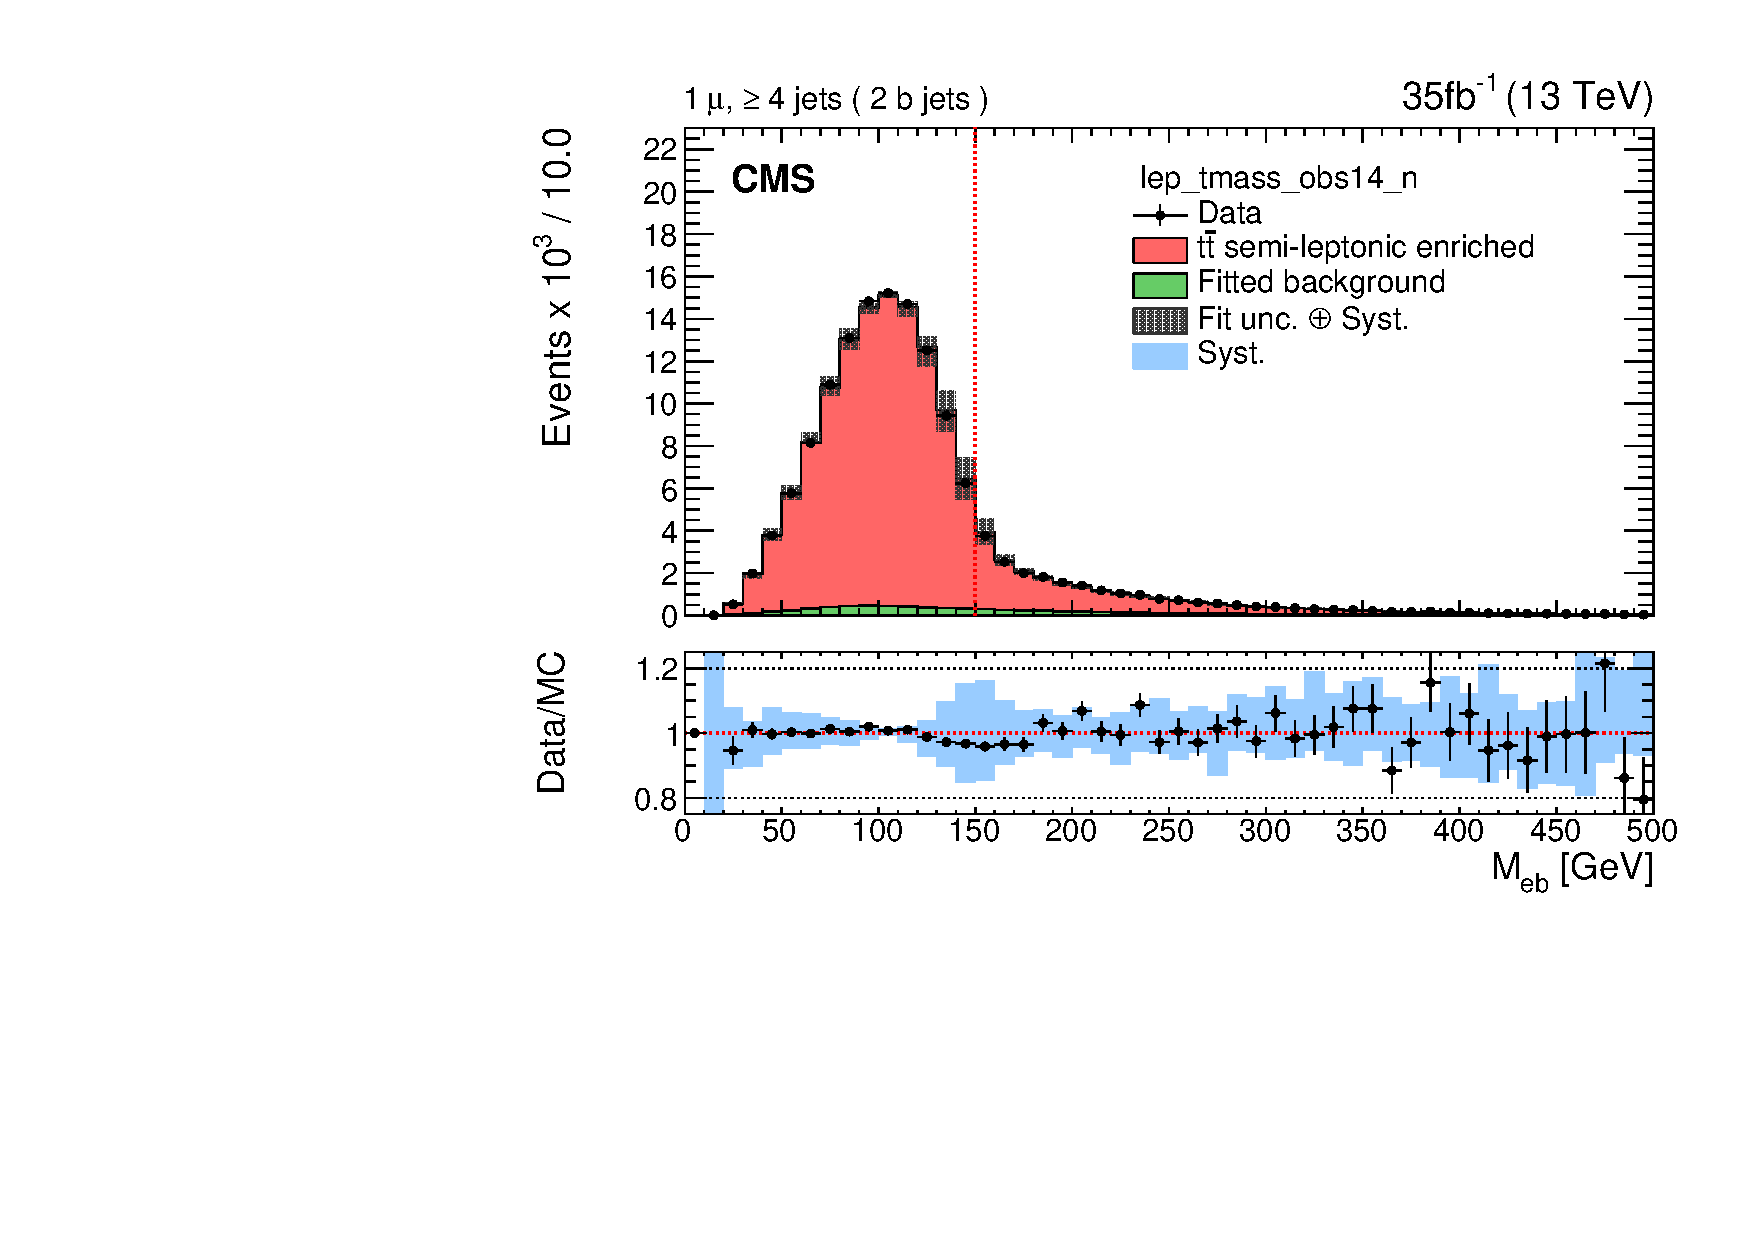
\includegraphics[width=0.4\textwidth]{figure/FitResult_16_mu_lep_tmass_obs14_n_chi2_20.pdf}
    \caption[The \Mlb invariant mass distributions in muon channel from 2016 data.]
    {
        The \Mlb invariant mass distributions in the positive (left) and negative (right) observable value region in muon channel from 2016 data (points).
        The results of the fit to the \ttbar and background templates are shown by the red and green histograms, respectively.
        The vertical bars on the data points in the upper panels indicate the statistical uncertainties in the data and the hatched bands show the combined statistical and systematic uncertainties in the simulation.
        The lower panels give the ratio of the data to the sum of the fitted MC predictions.
        The blue bands represent the systematic uncertainties in the expected yield in the simulation for all sources of systematic uncertainty (Section~\ref{sec:uncertainty}).
    }
    \label{fig:fitting_results_16_mu}
\end{figure}
\begin{figure}
    \centering
    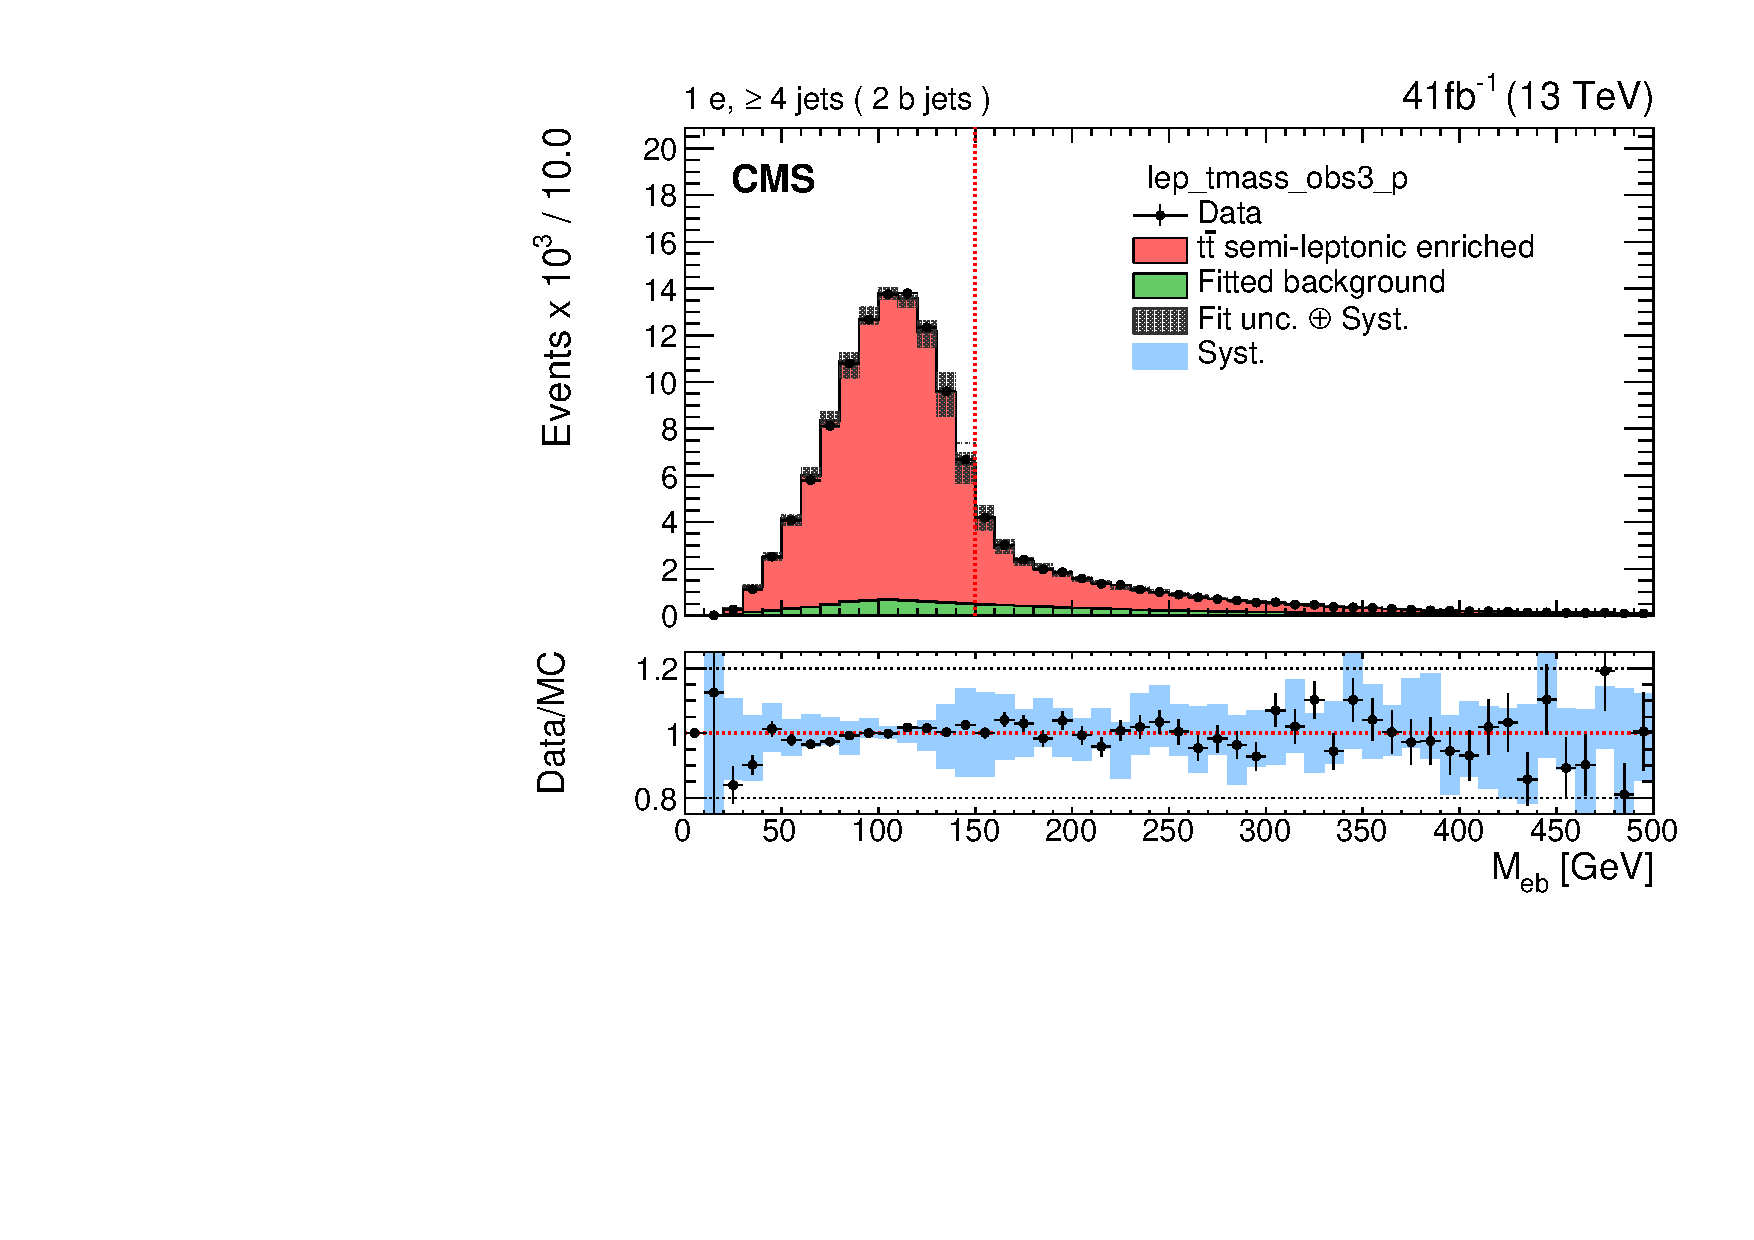
\includegraphics[width=0.4\textwidth]{figure/FitResult_17_el_lep_tmass_obs3_p_chi2_20.pdf}
    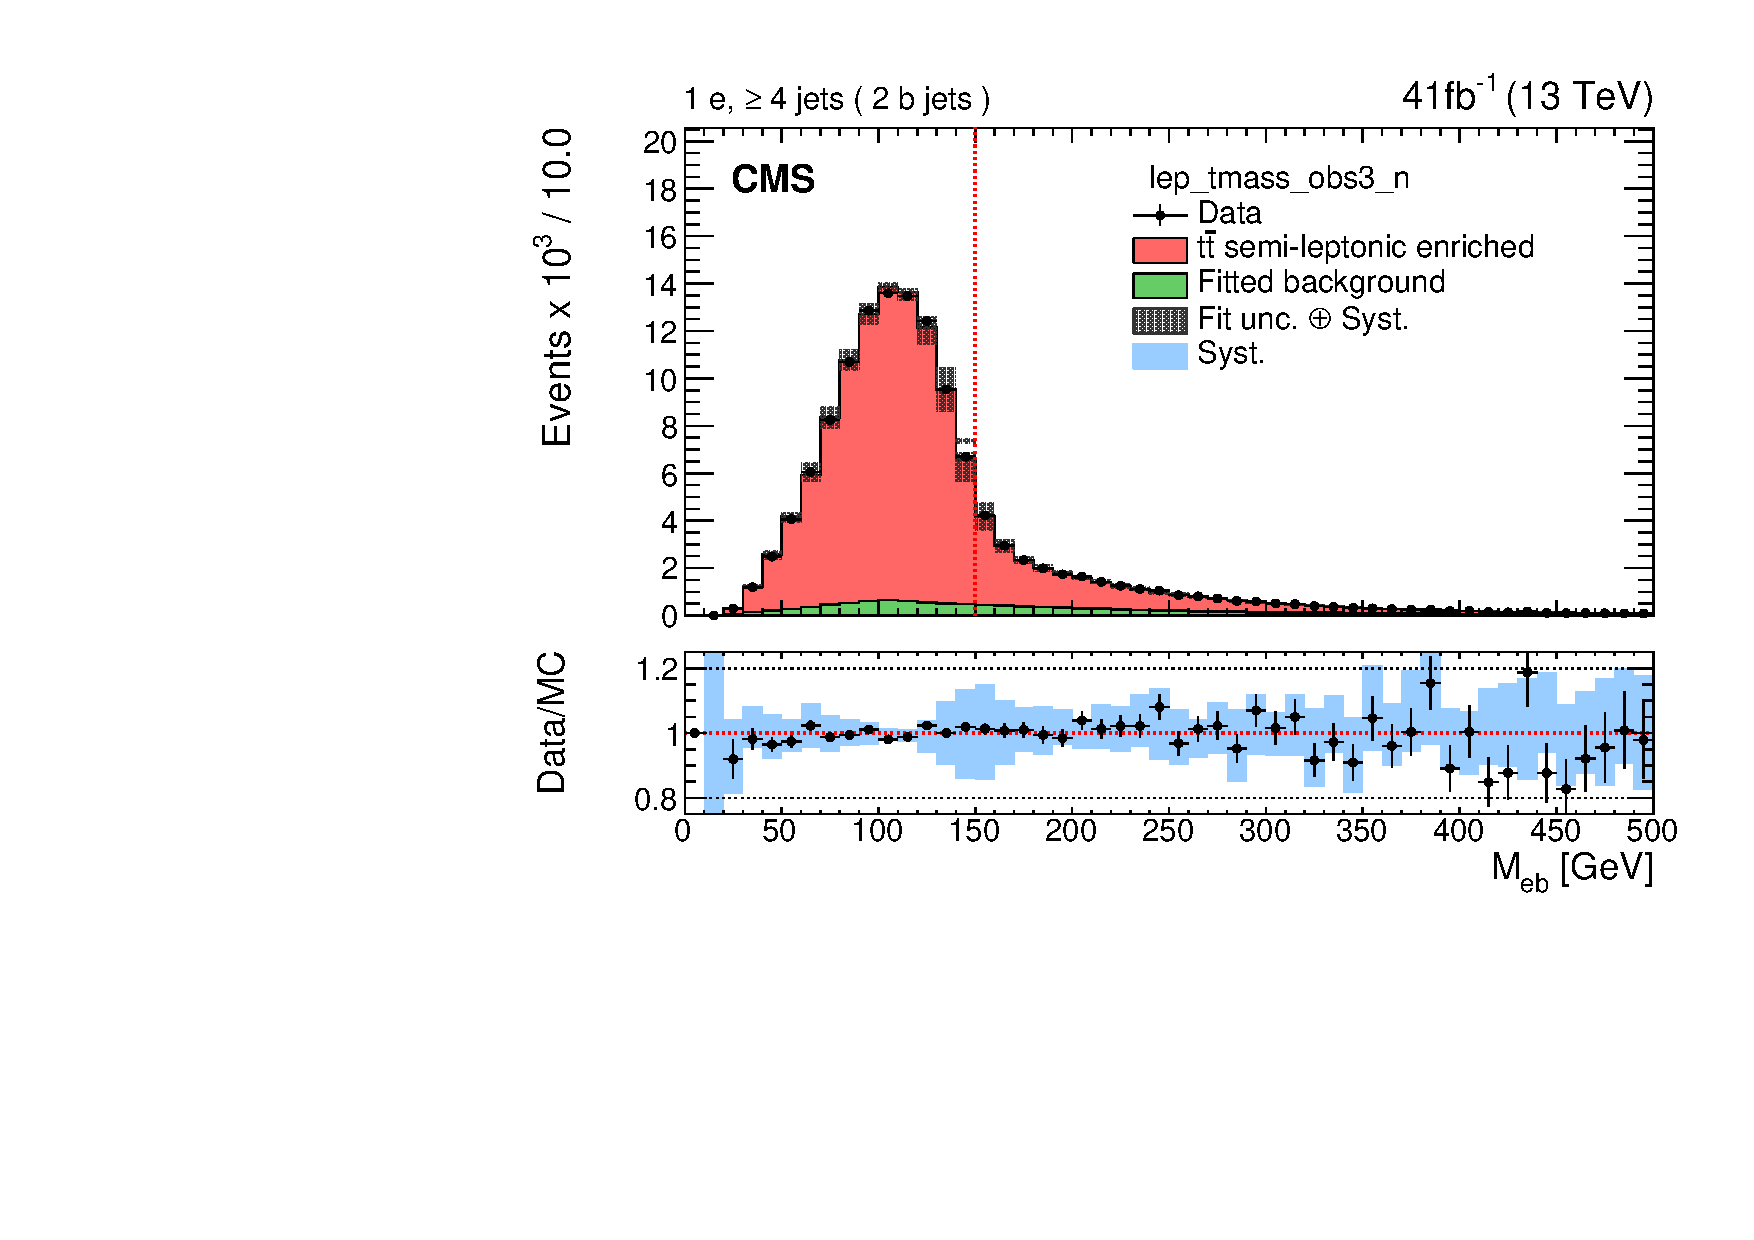
\includegraphics[width=0.4\textwidth]{figure/FitResult_17_el_lep_tmass_obs3_n_chi2_20.pdf}
    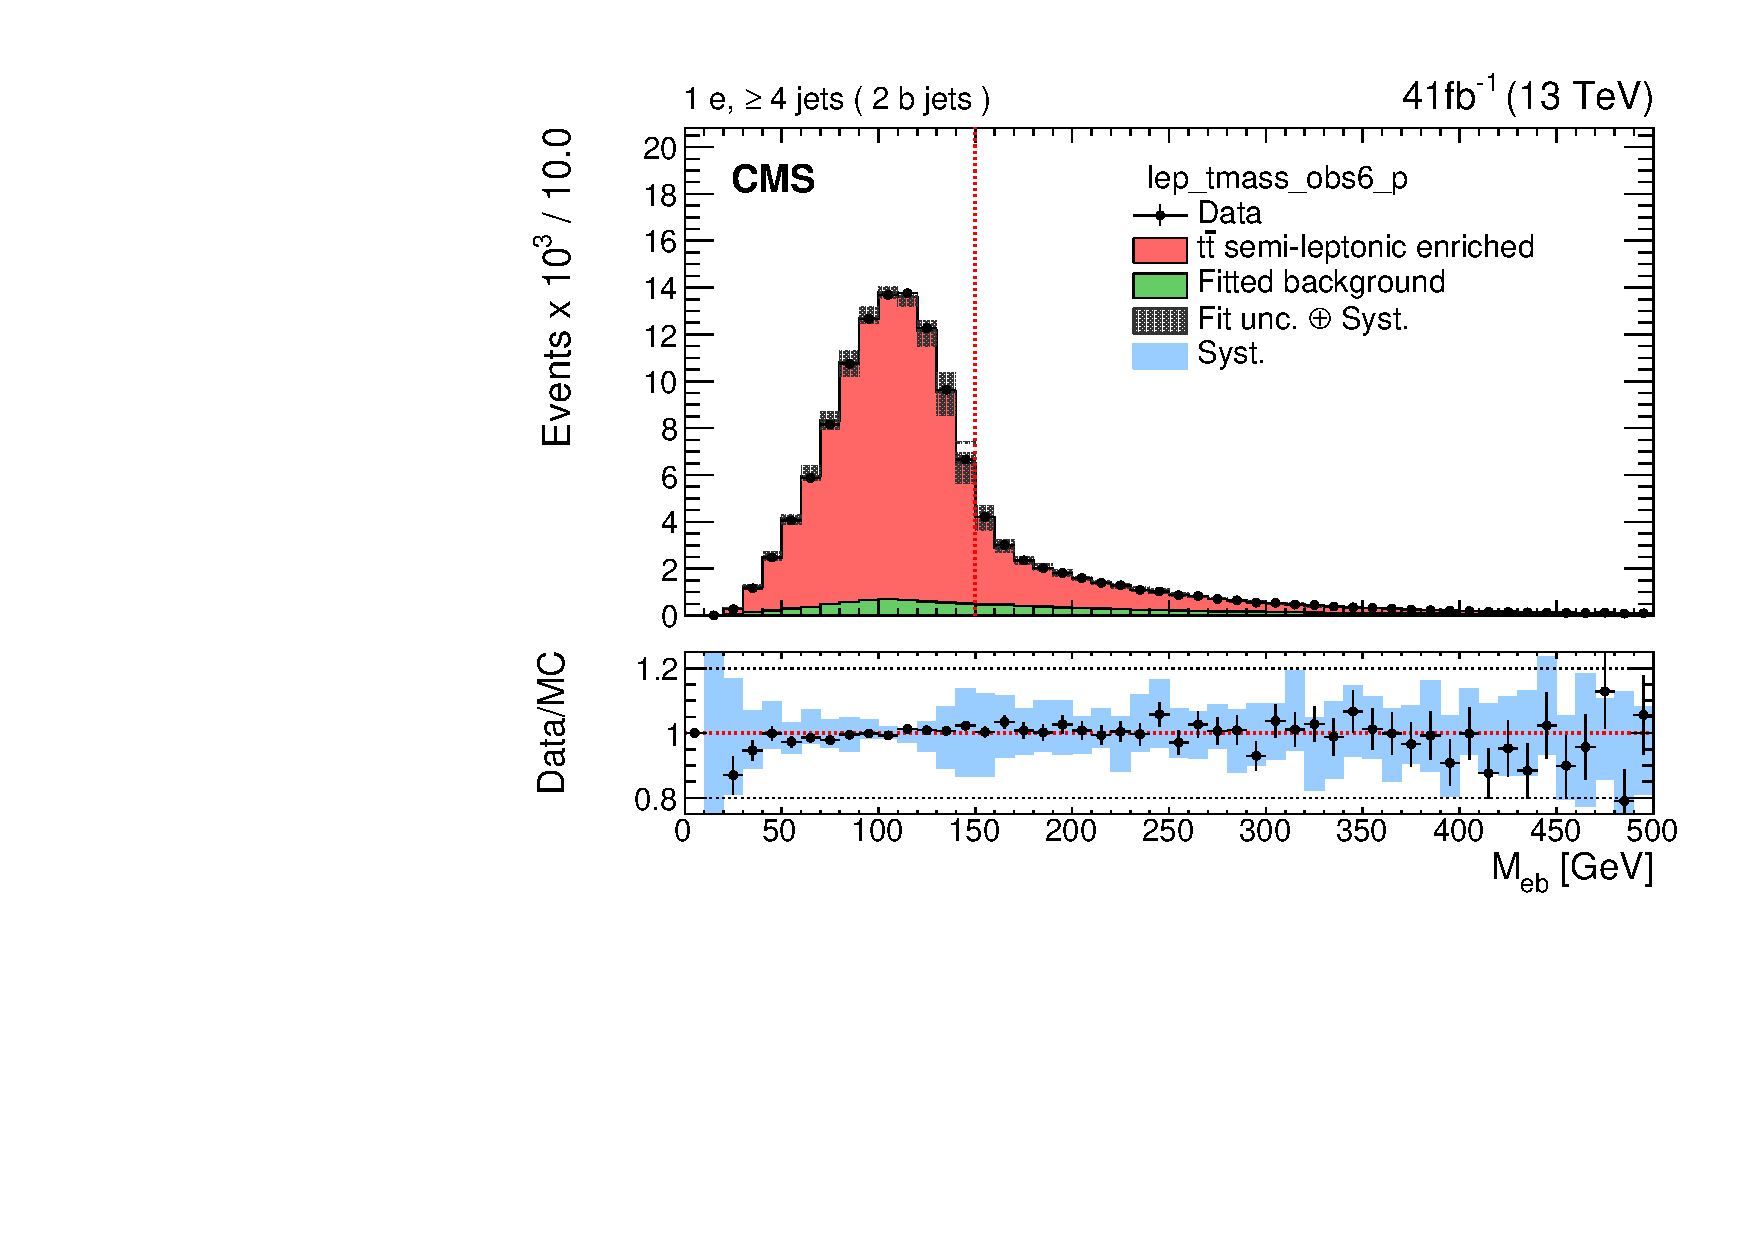
\includegraphics[width=0.4\textwidth]{figure/FitResult_17_el_lep_tmass_obs6_p_chi2_20.pdf}
    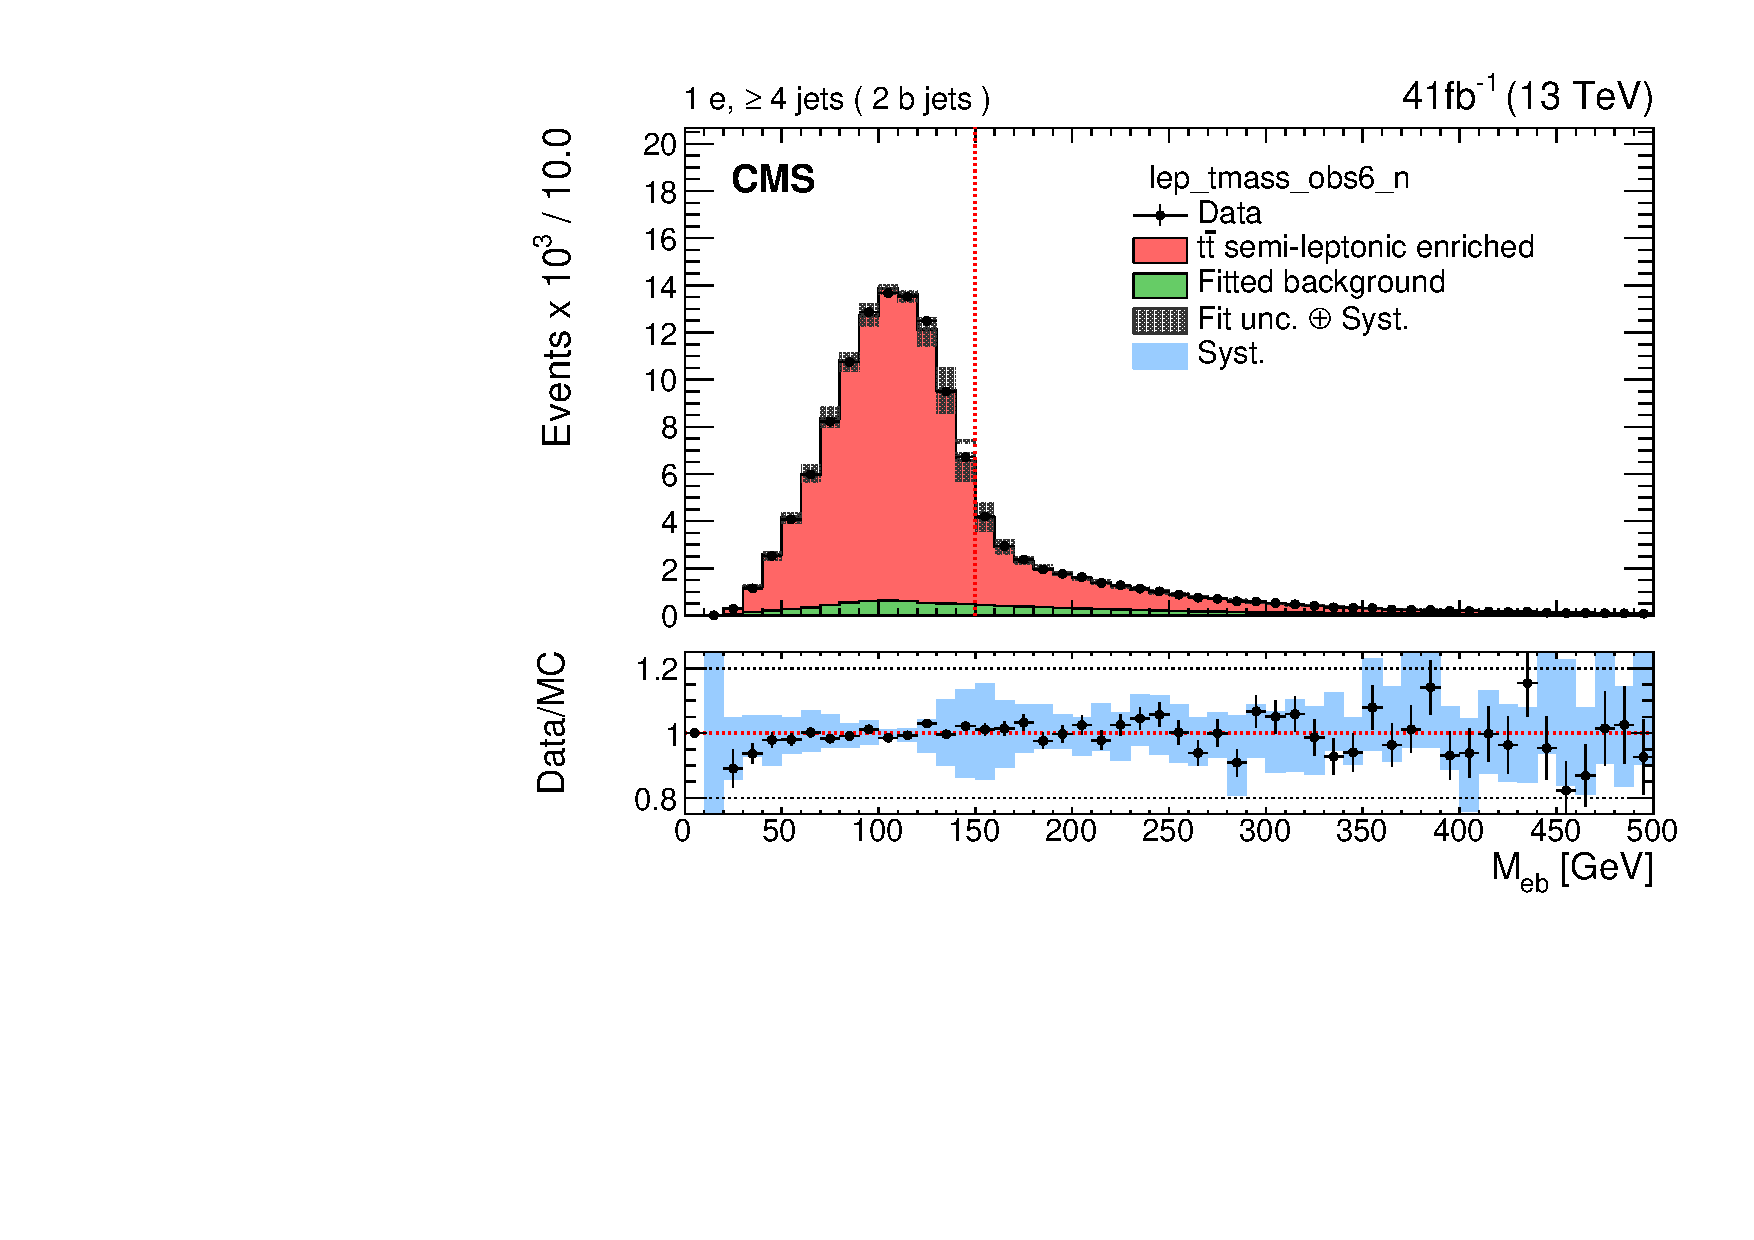
\includegraphics[width=0.4\textwidth]{figure/FitResult_17_el_lep_tmass_obs6_n_chi2_20.pdf}
    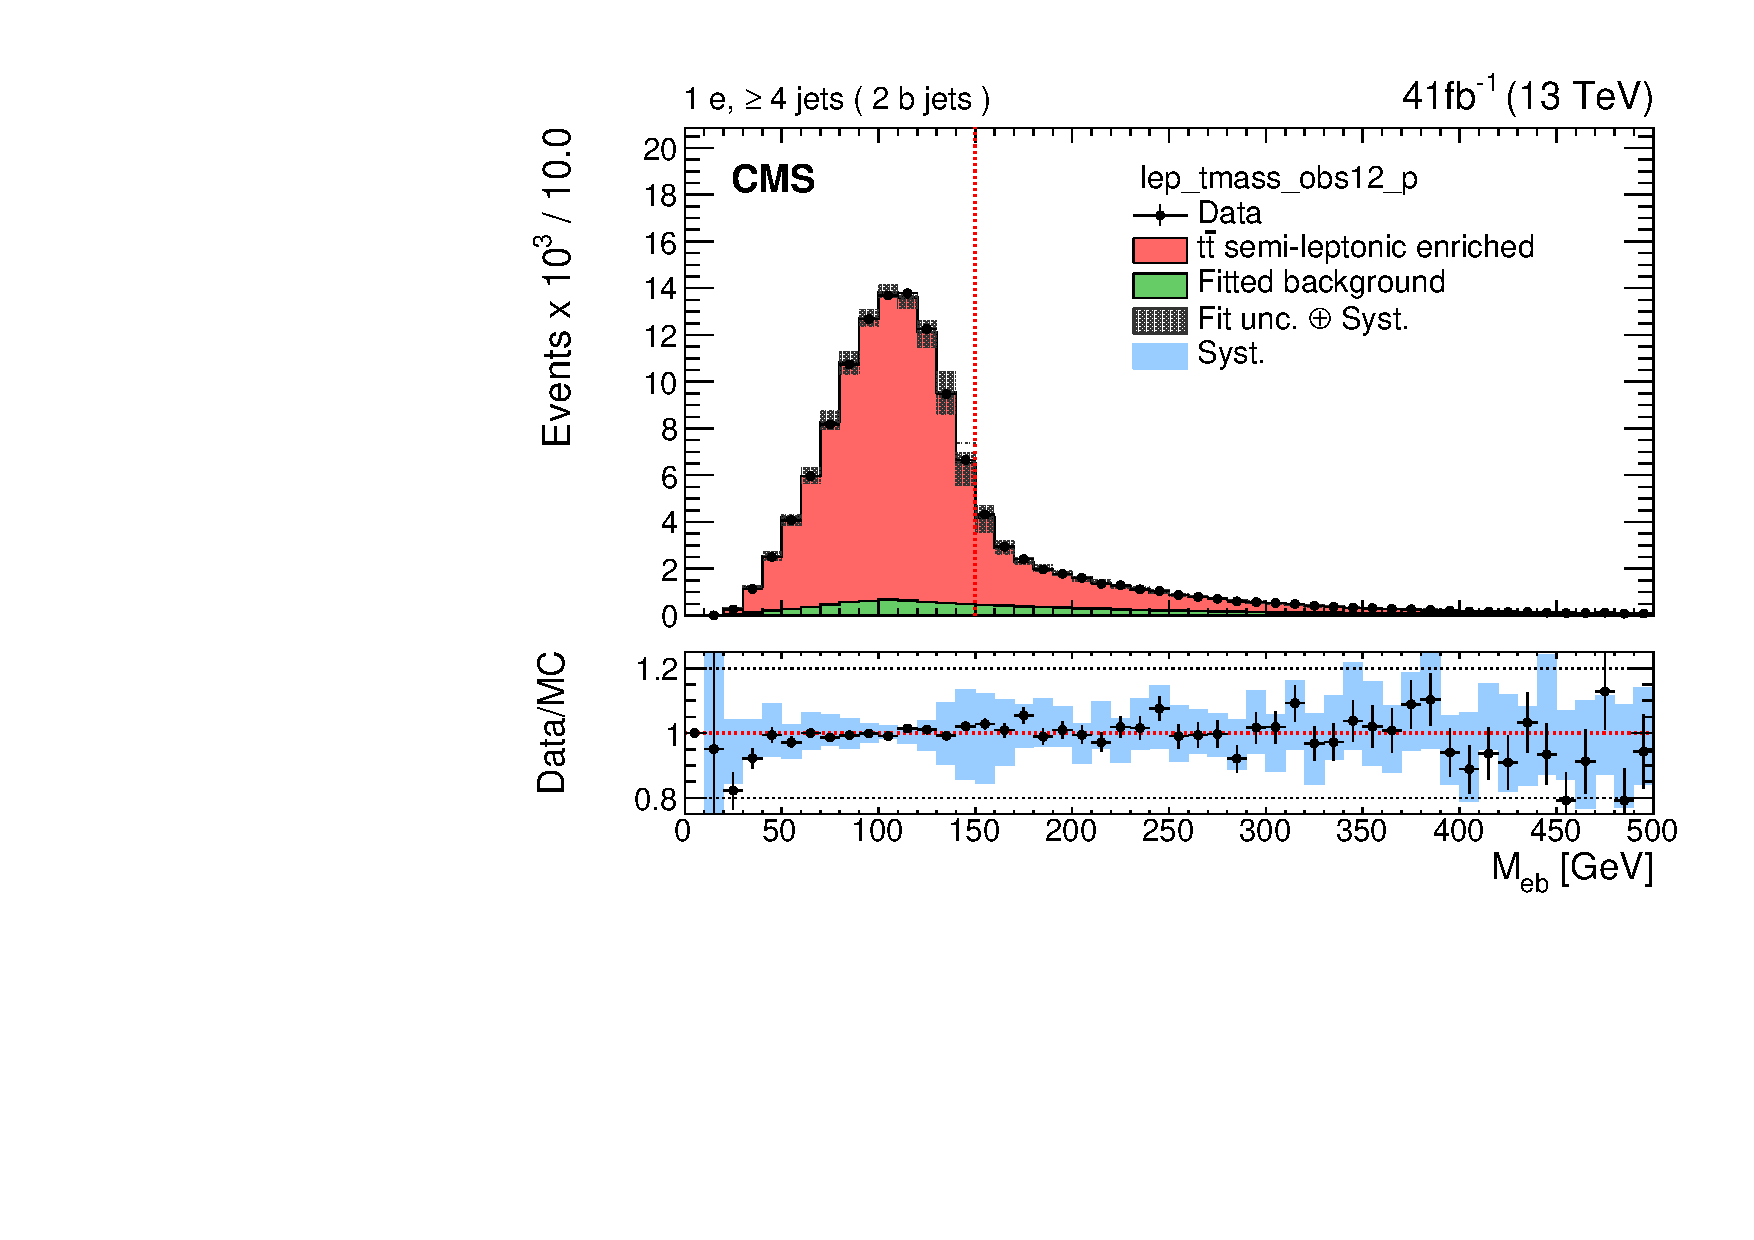
\includegraphics[width=0.4\textwidth]{figure/FitResult_17_el_lep_tmass_obs12_p_chi2_20.pdf}
    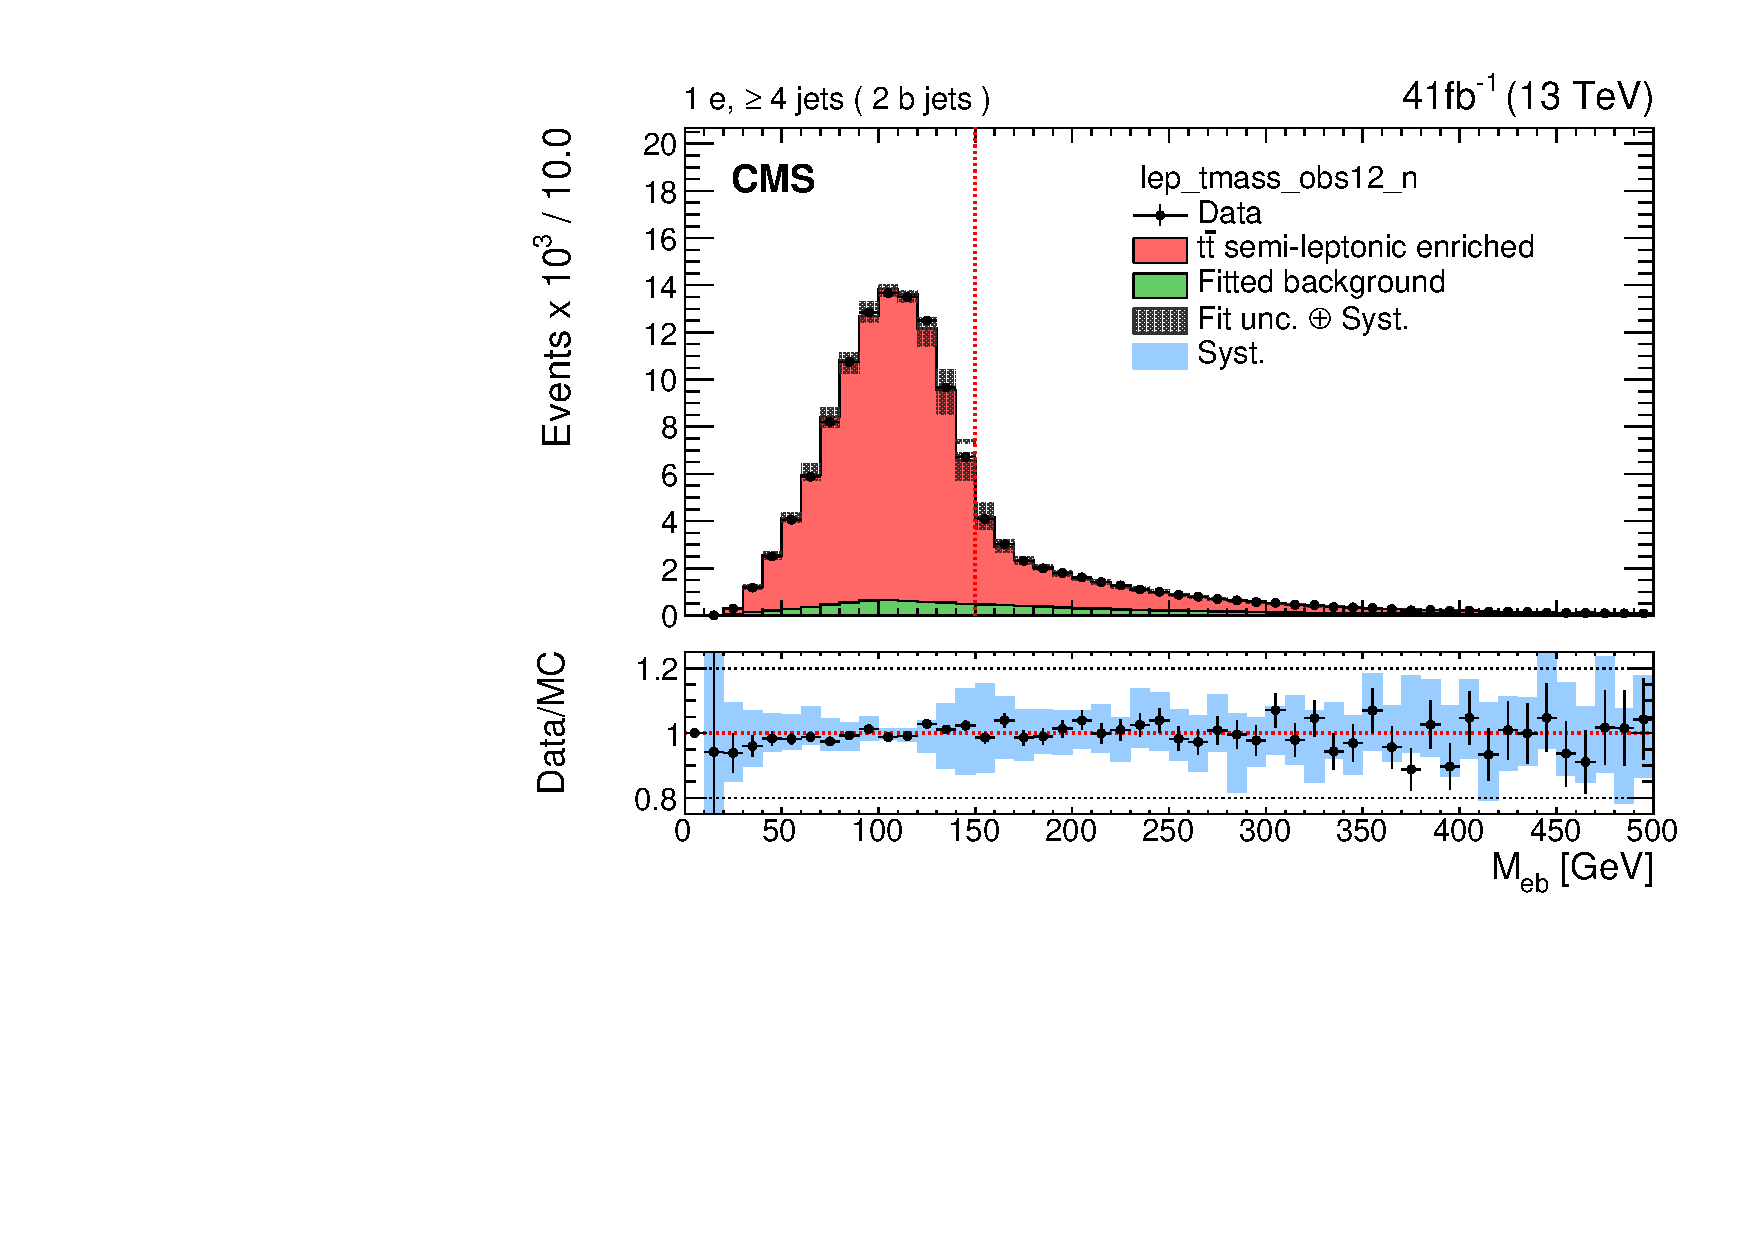
\includegraphics[width=0.4\textwidth]{figure/FitResult_17_el_lep_tmass_obs12_n_chi2_20.pdf}
    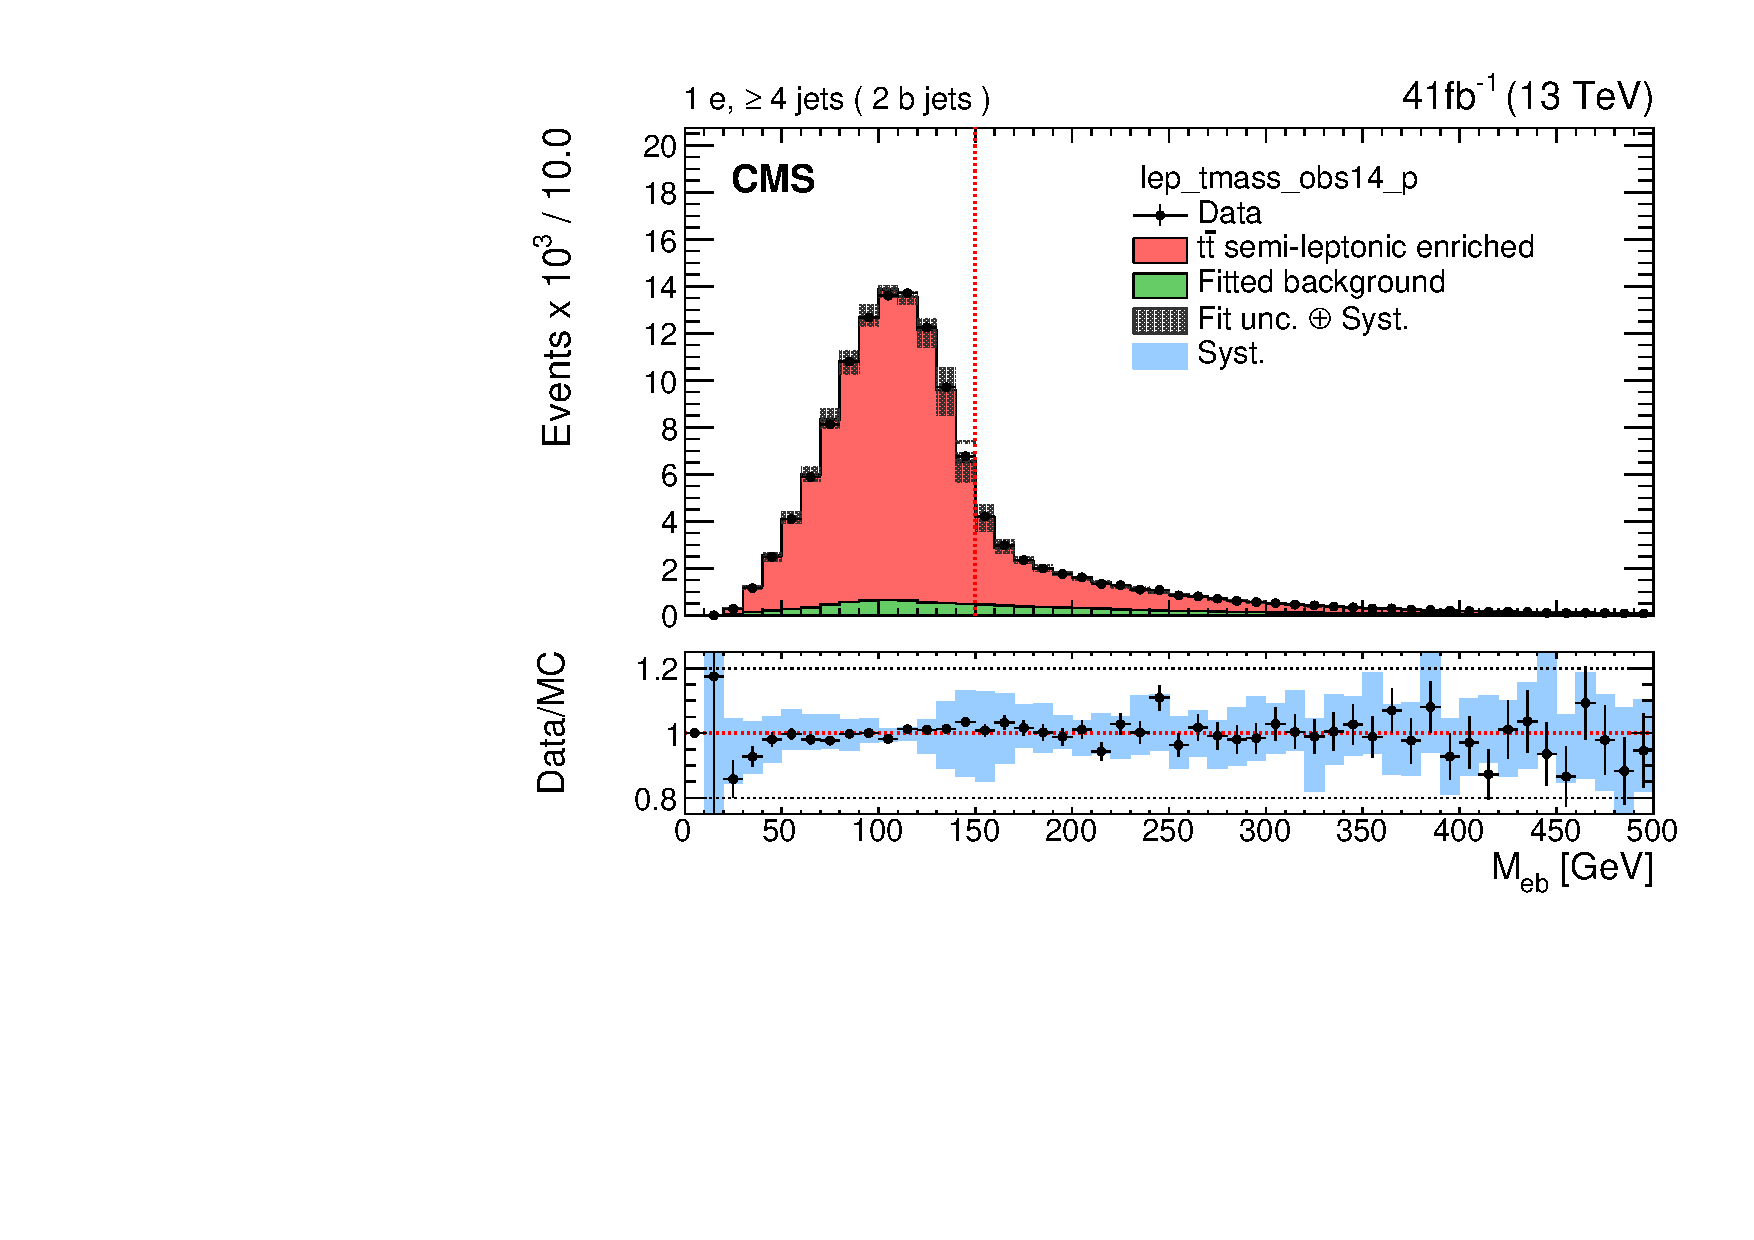
\includegraphics[width=0.4\textwidth]{figure/FitResult_17_el_lep_tmass_obs14_p_chi2_20.pdf}
    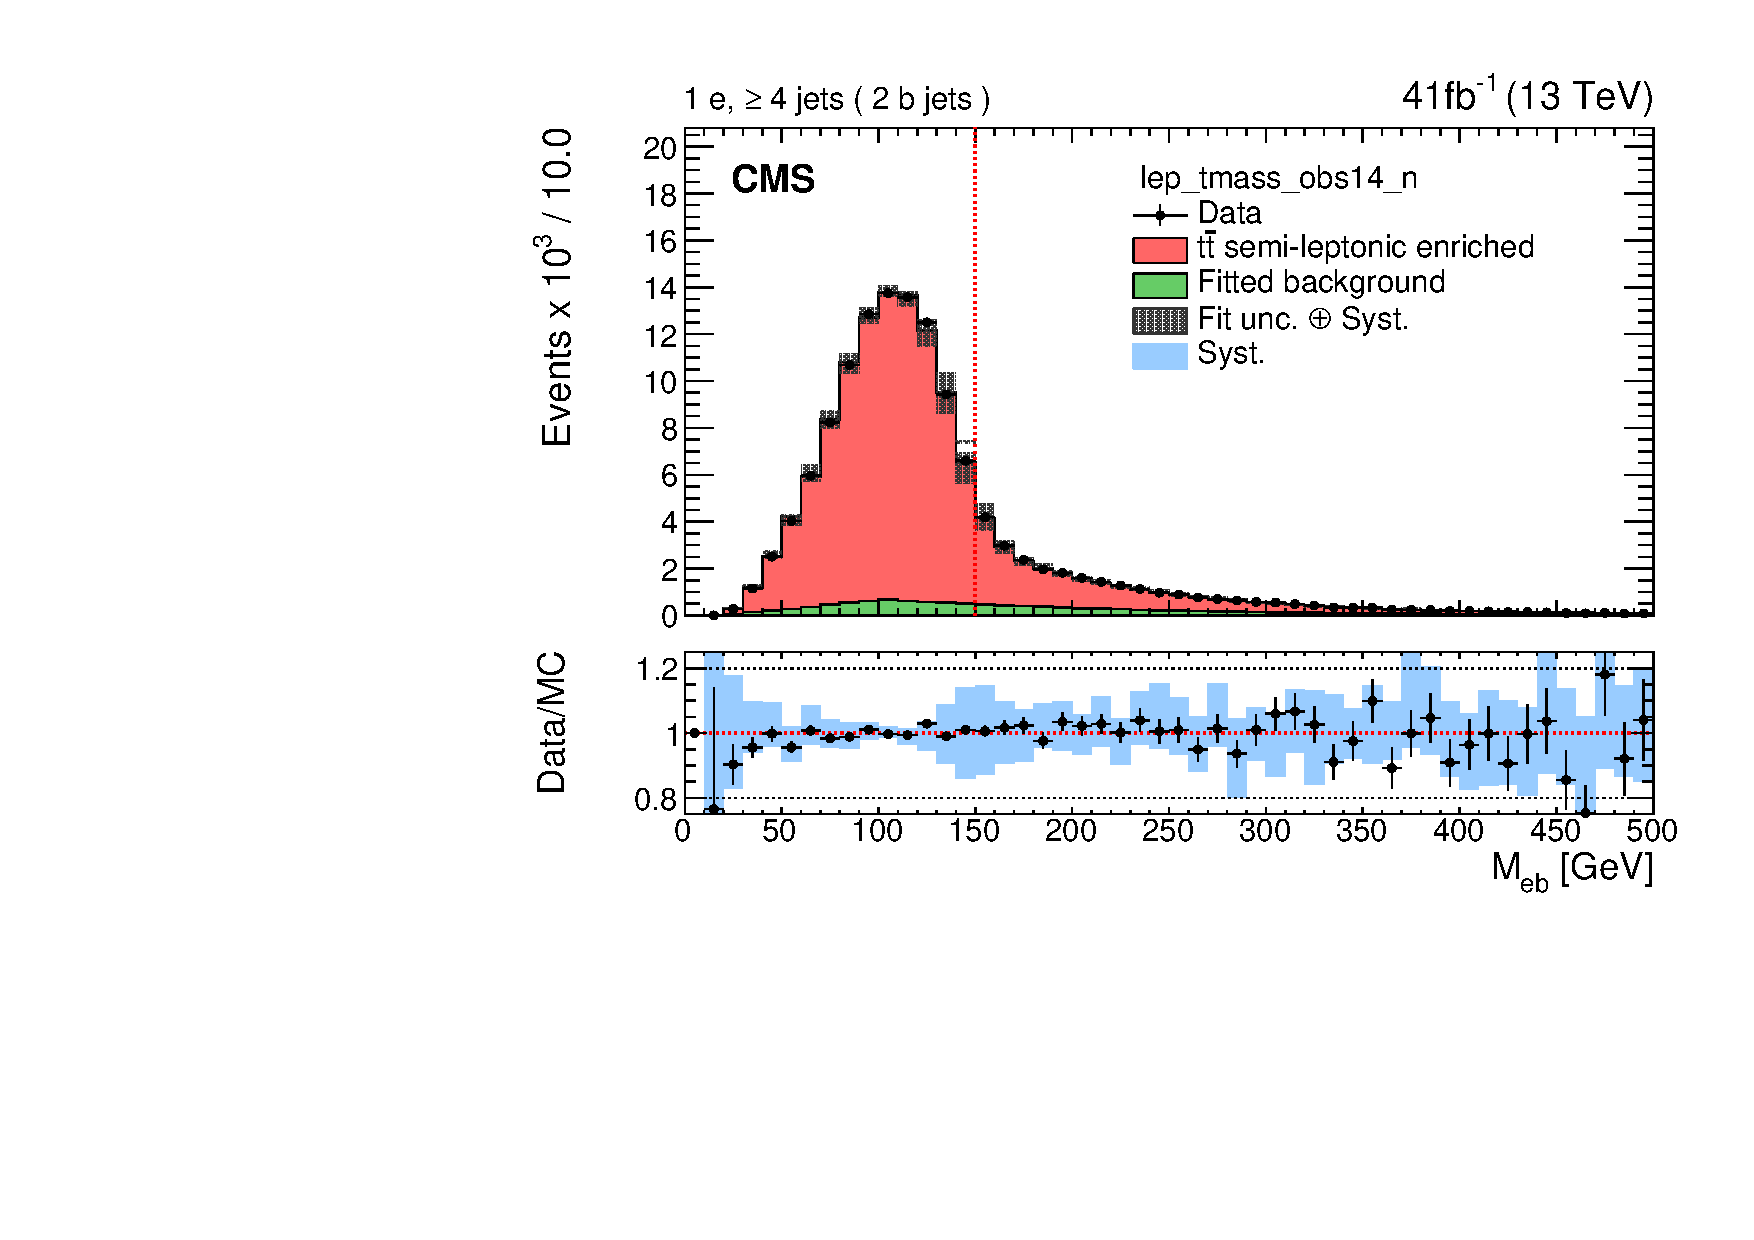
\includegraphics[width=0.4\textwidth]{figure/FitResult_17_el_lep_tmass_obs14_n_chi2_20.pdf}
    \caption[The \Mlb invariant mass distributions in electron channel from 2017 data.]
    {
        The \Mlb invariant mass distributions in the positive (left) and negative (right) observable value region in electron channel from 2017 data (points).
        The results of the fit to the \ttbar and background templates are shown by the red and green histograms, respectively.
        The vertical bars on the data points in the upper panels indicate the statistical uncertainties in the data and the hatched bands show the combined statistical and systematic uncertainties in the simulation.
        The lower panels give the ratio of the data to the sum of the fitted MC predictions.
        The blue bands represent the systematic uncertainties in the expected yield in the simulation for all sources of systematic uncertainty (Section~\ref{sec:uncertainty}).
    }
    \label{fig:fitting_results_17_el}
\end{figure}
\begin{figure}
    \centering
    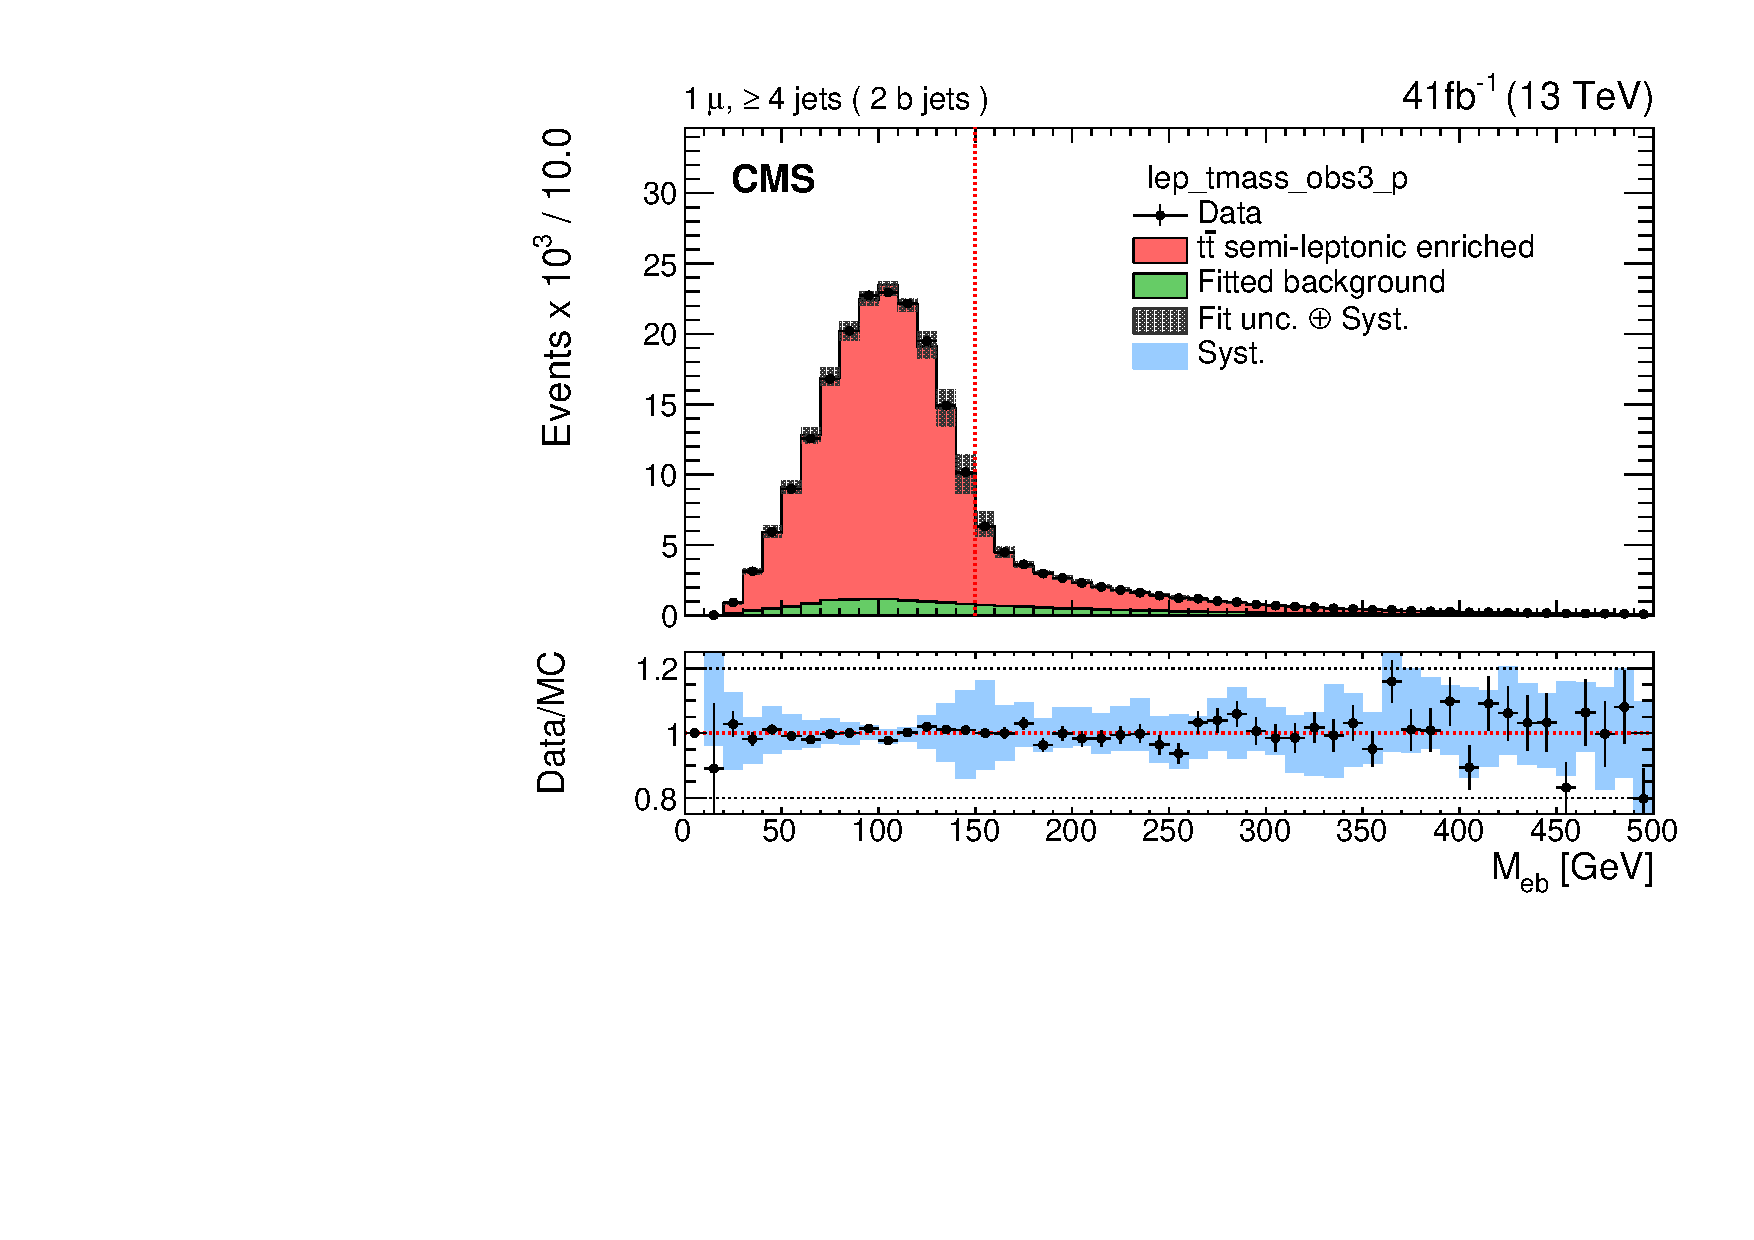
\includegraphics[width=0.4\textwidth]{figure/FitResult_17_mu_lep_tmass_obs3_p_chi2_20.pdf}
    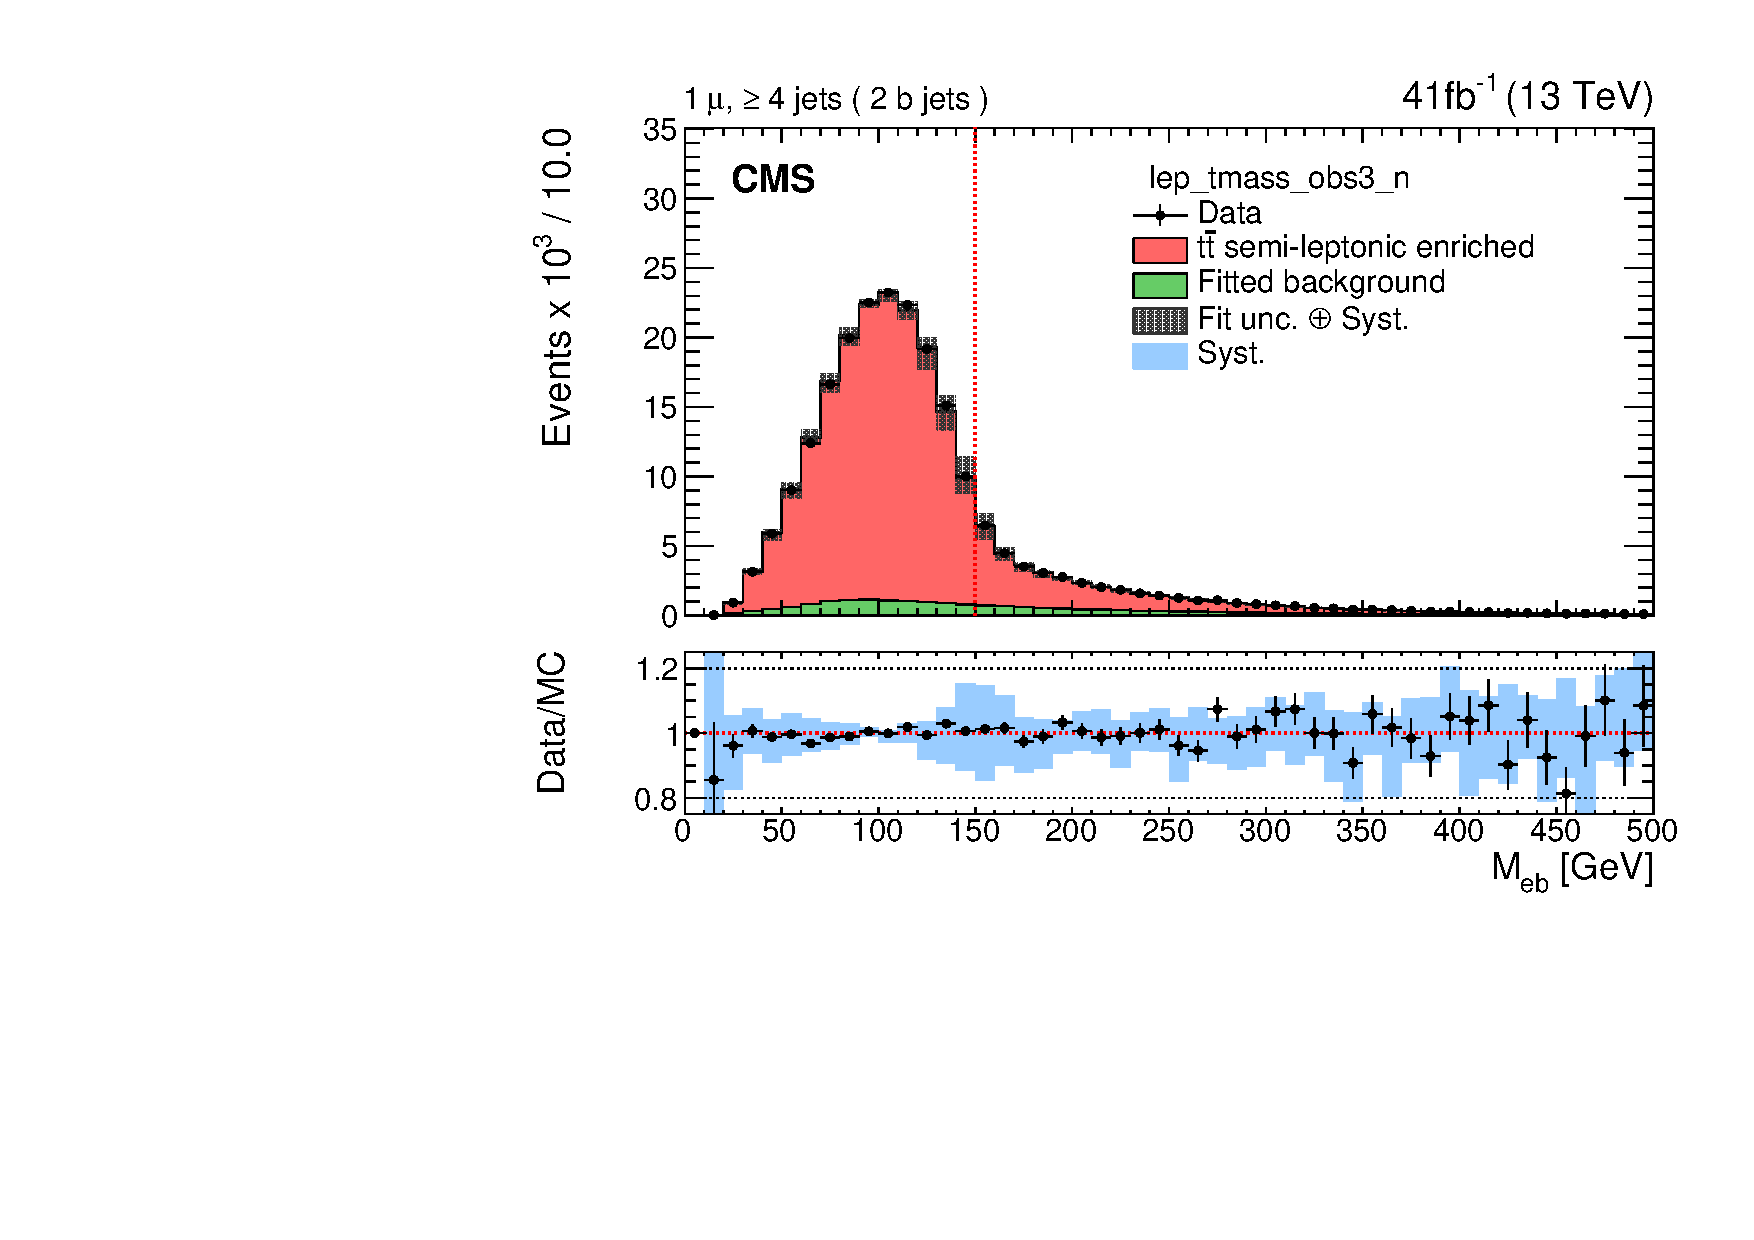
\includegraphics[width=0.4\textwidth]{figure/FitResult_17_mu_lep_tmass_obs3_n_chi2_20.pdf}
    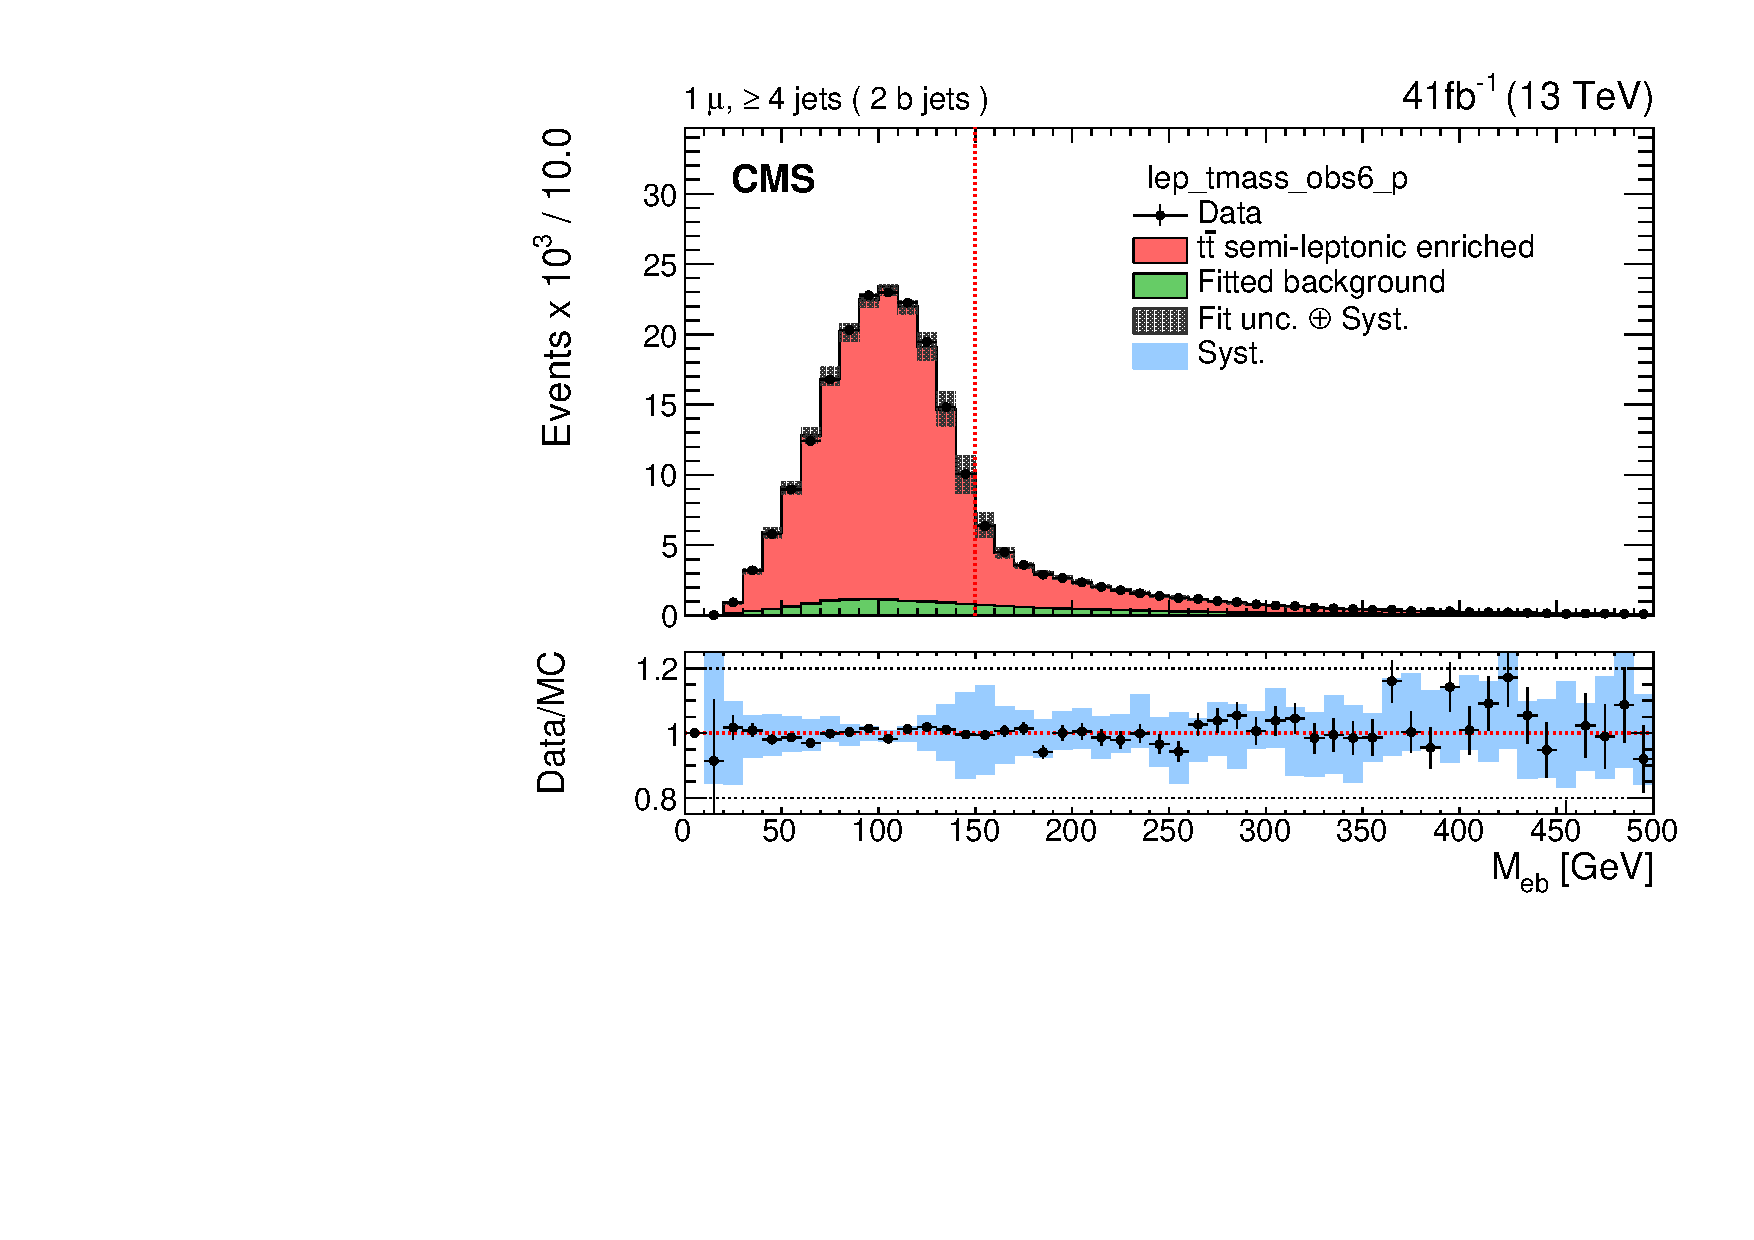
\includegraphics[width=0.4\textwidth]{figure/FitResult_17_mu_lep_tmass_obs6_p_chi2_20.pdf}
    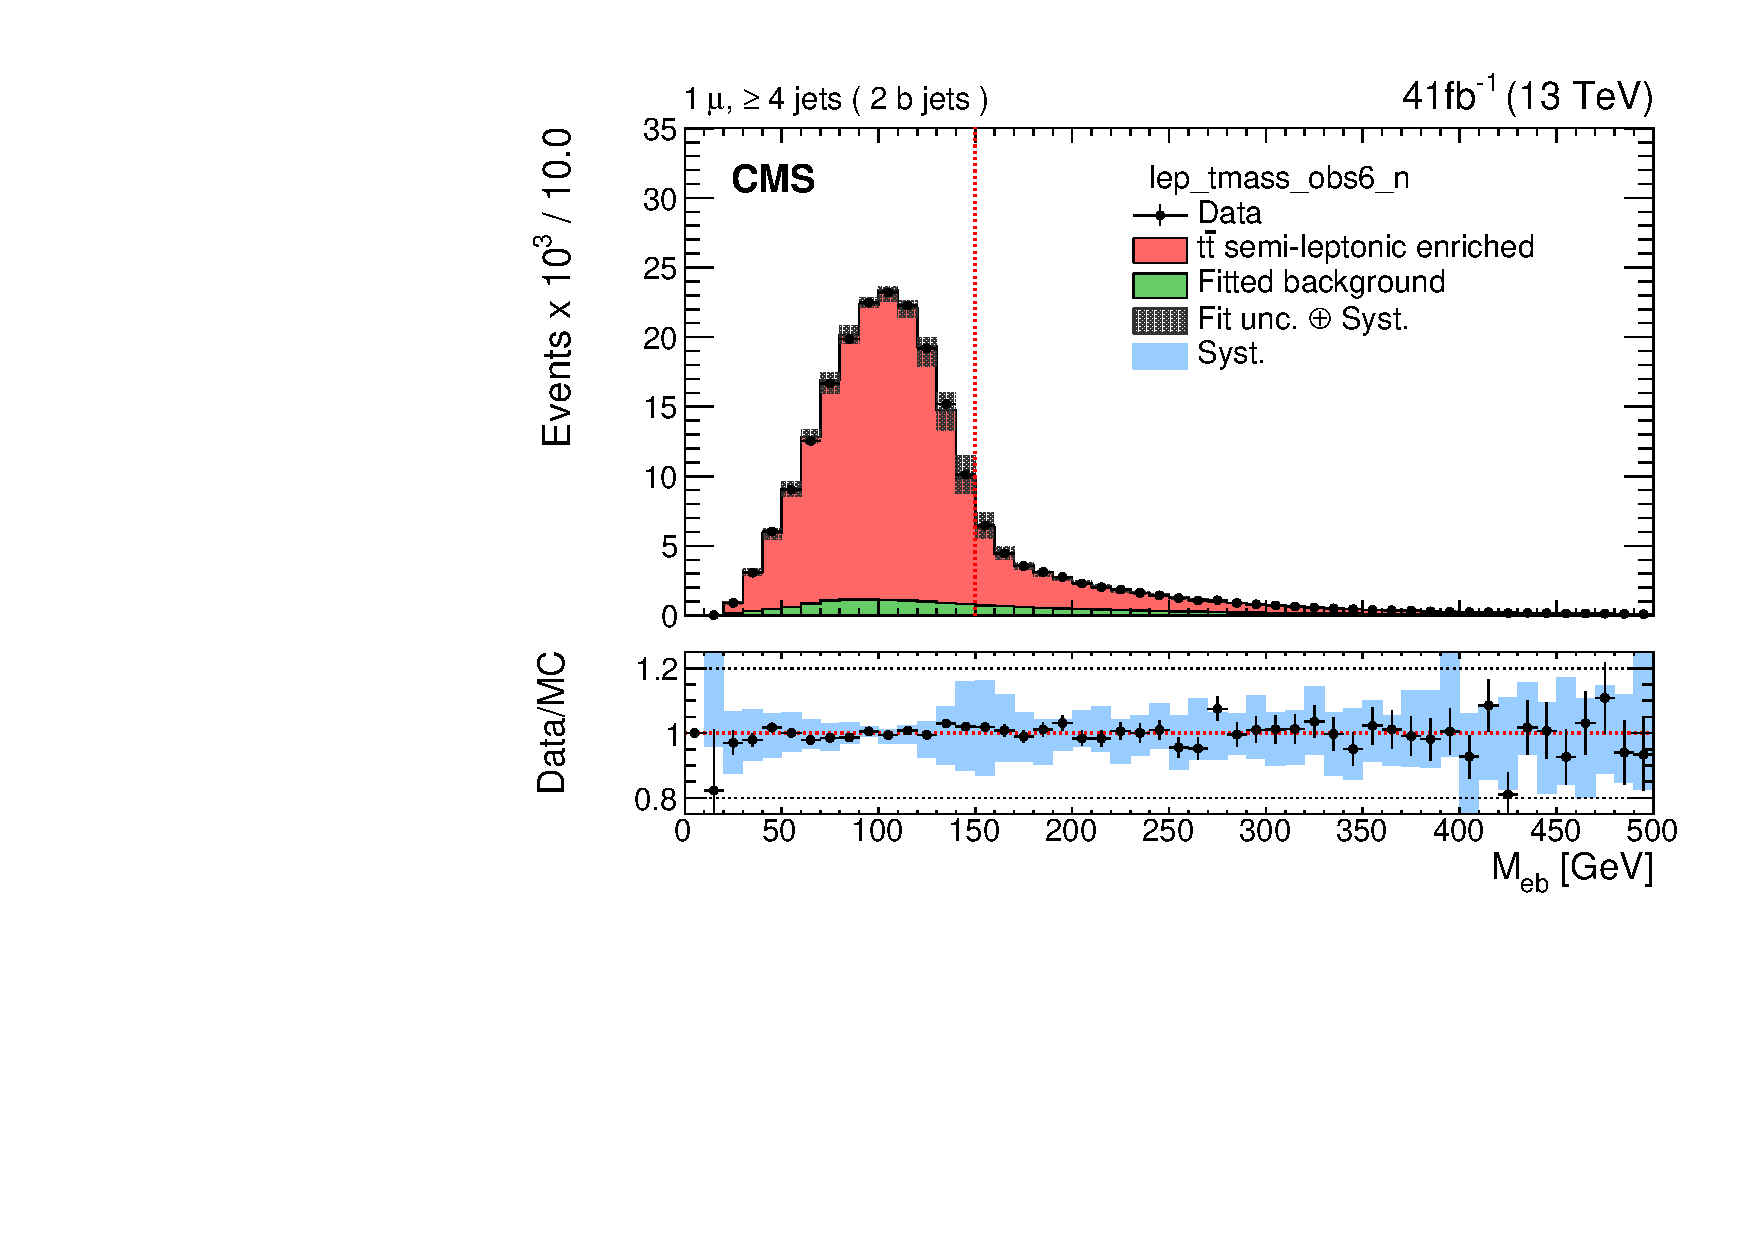
\includegraphics[width=0.4\textwidth]{figure/FitResult_17_mu_lep_tmass_obs6_n_chi2_20.pdf}
    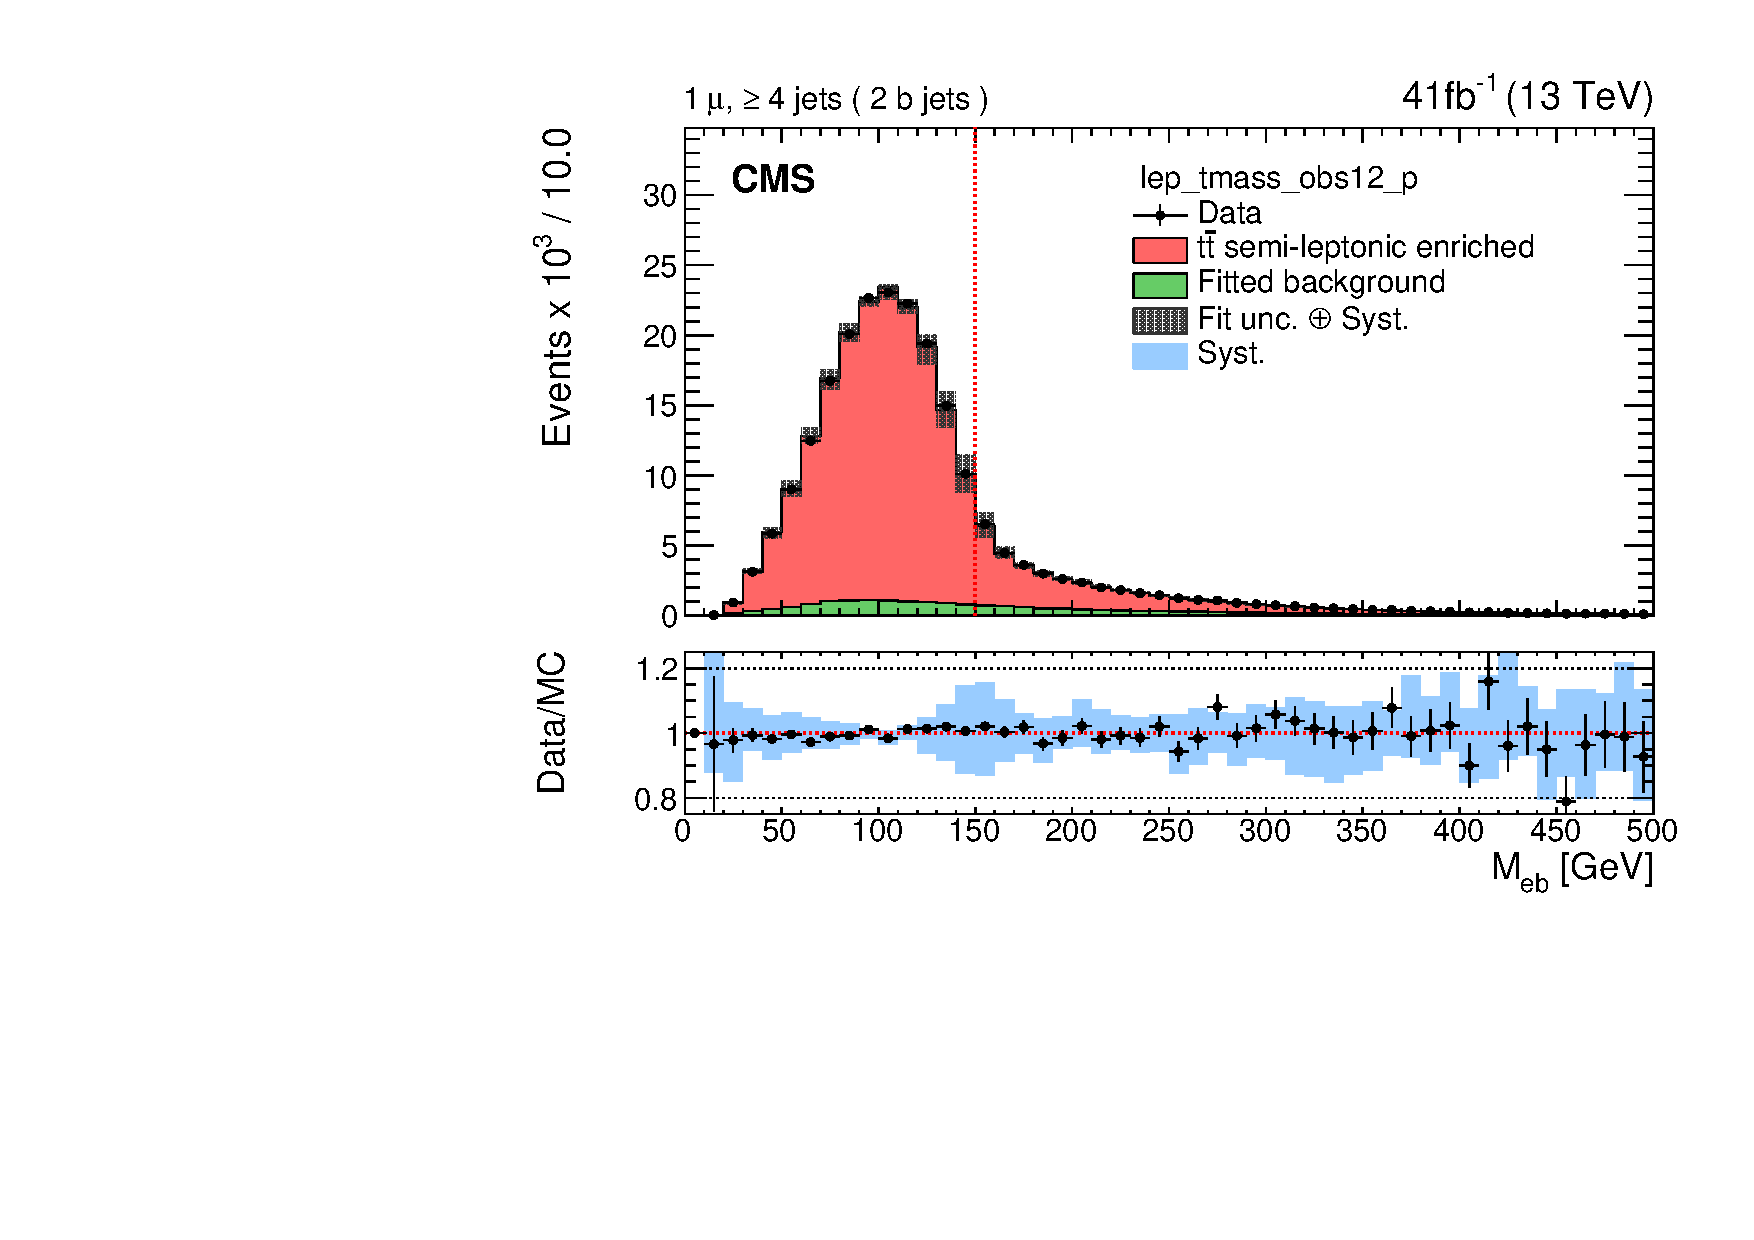
\includegraphics[width=0.4\textwidth]{figure/FitResult_17_mu_lep_tmass_obs12_p_chi2_20.pdf}
    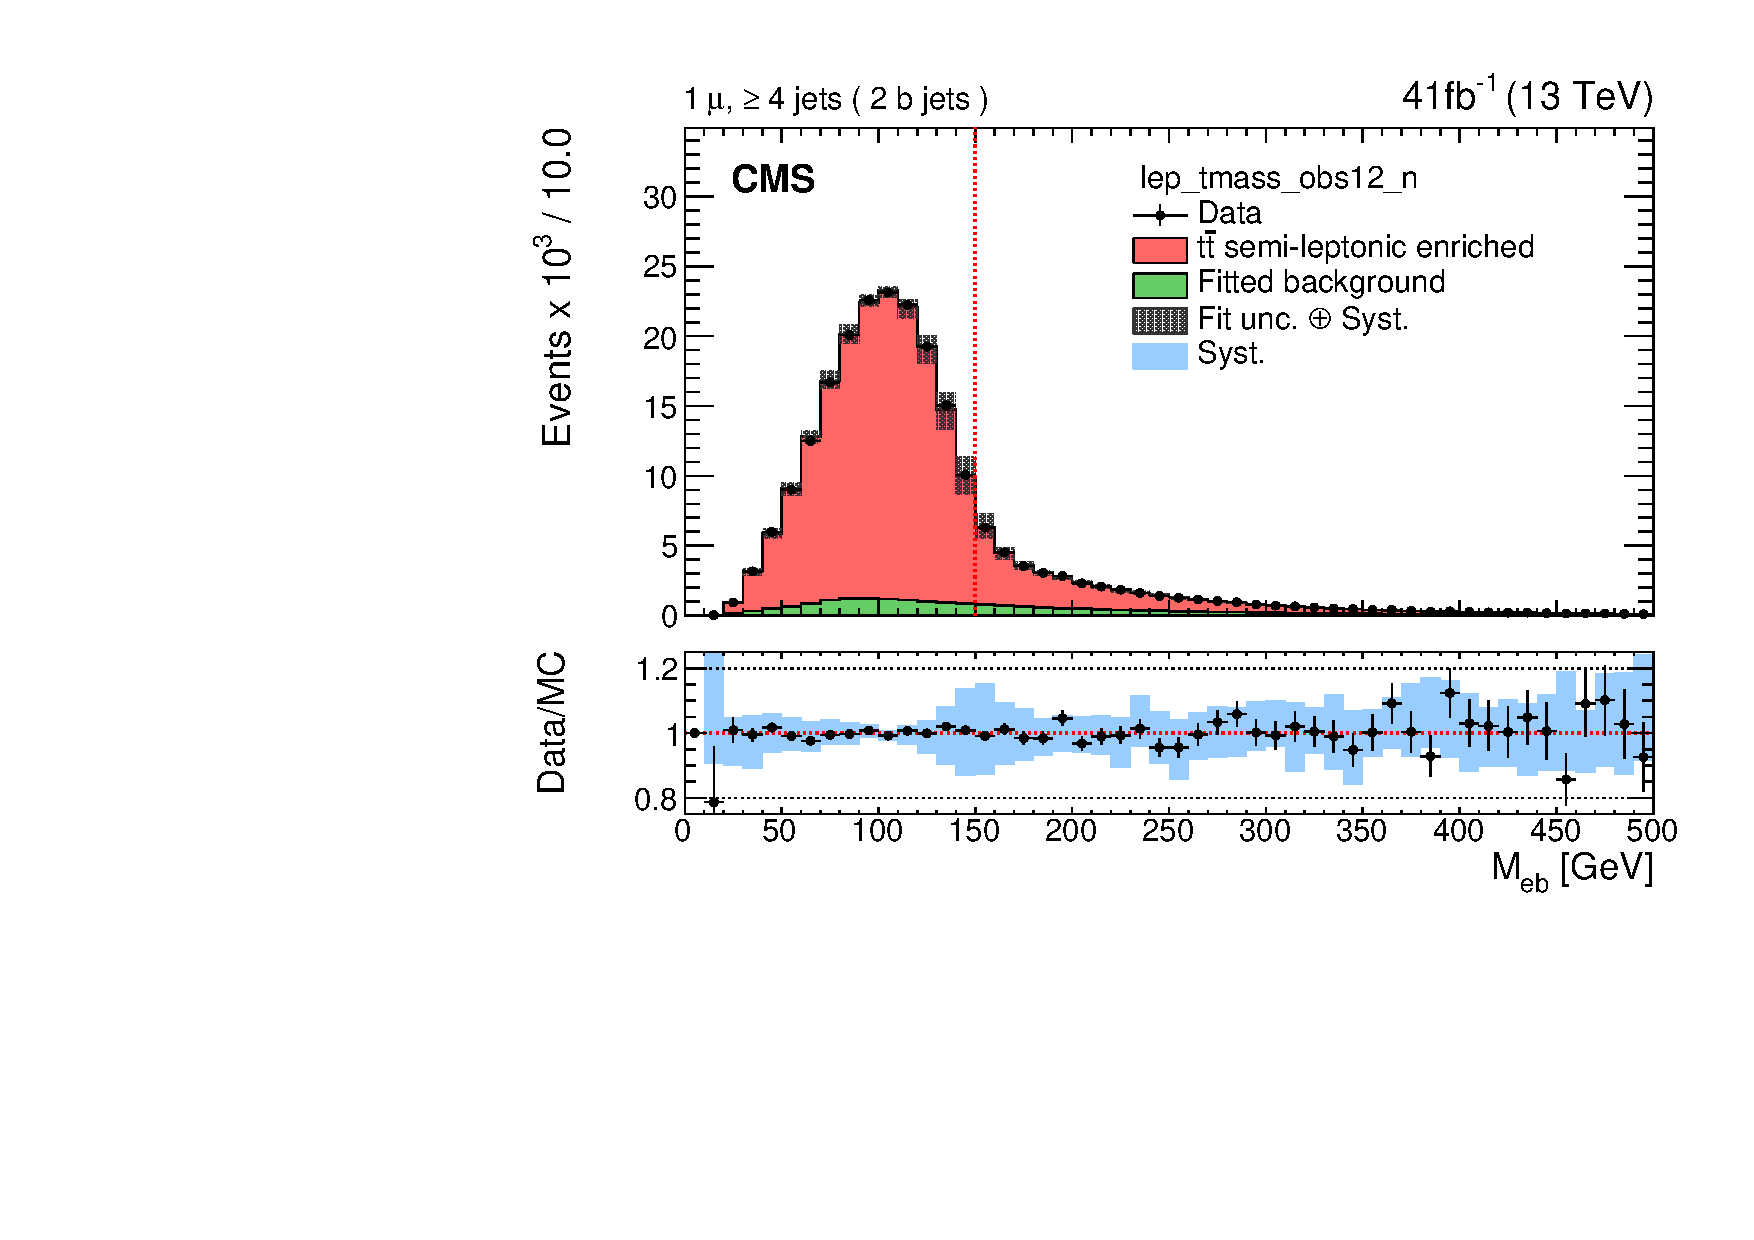
\includegraphics[width=0.4\textwidth]{figure/FitResult_17_mu_lep_tmass_obs12_n_chi2_20.pdf}
    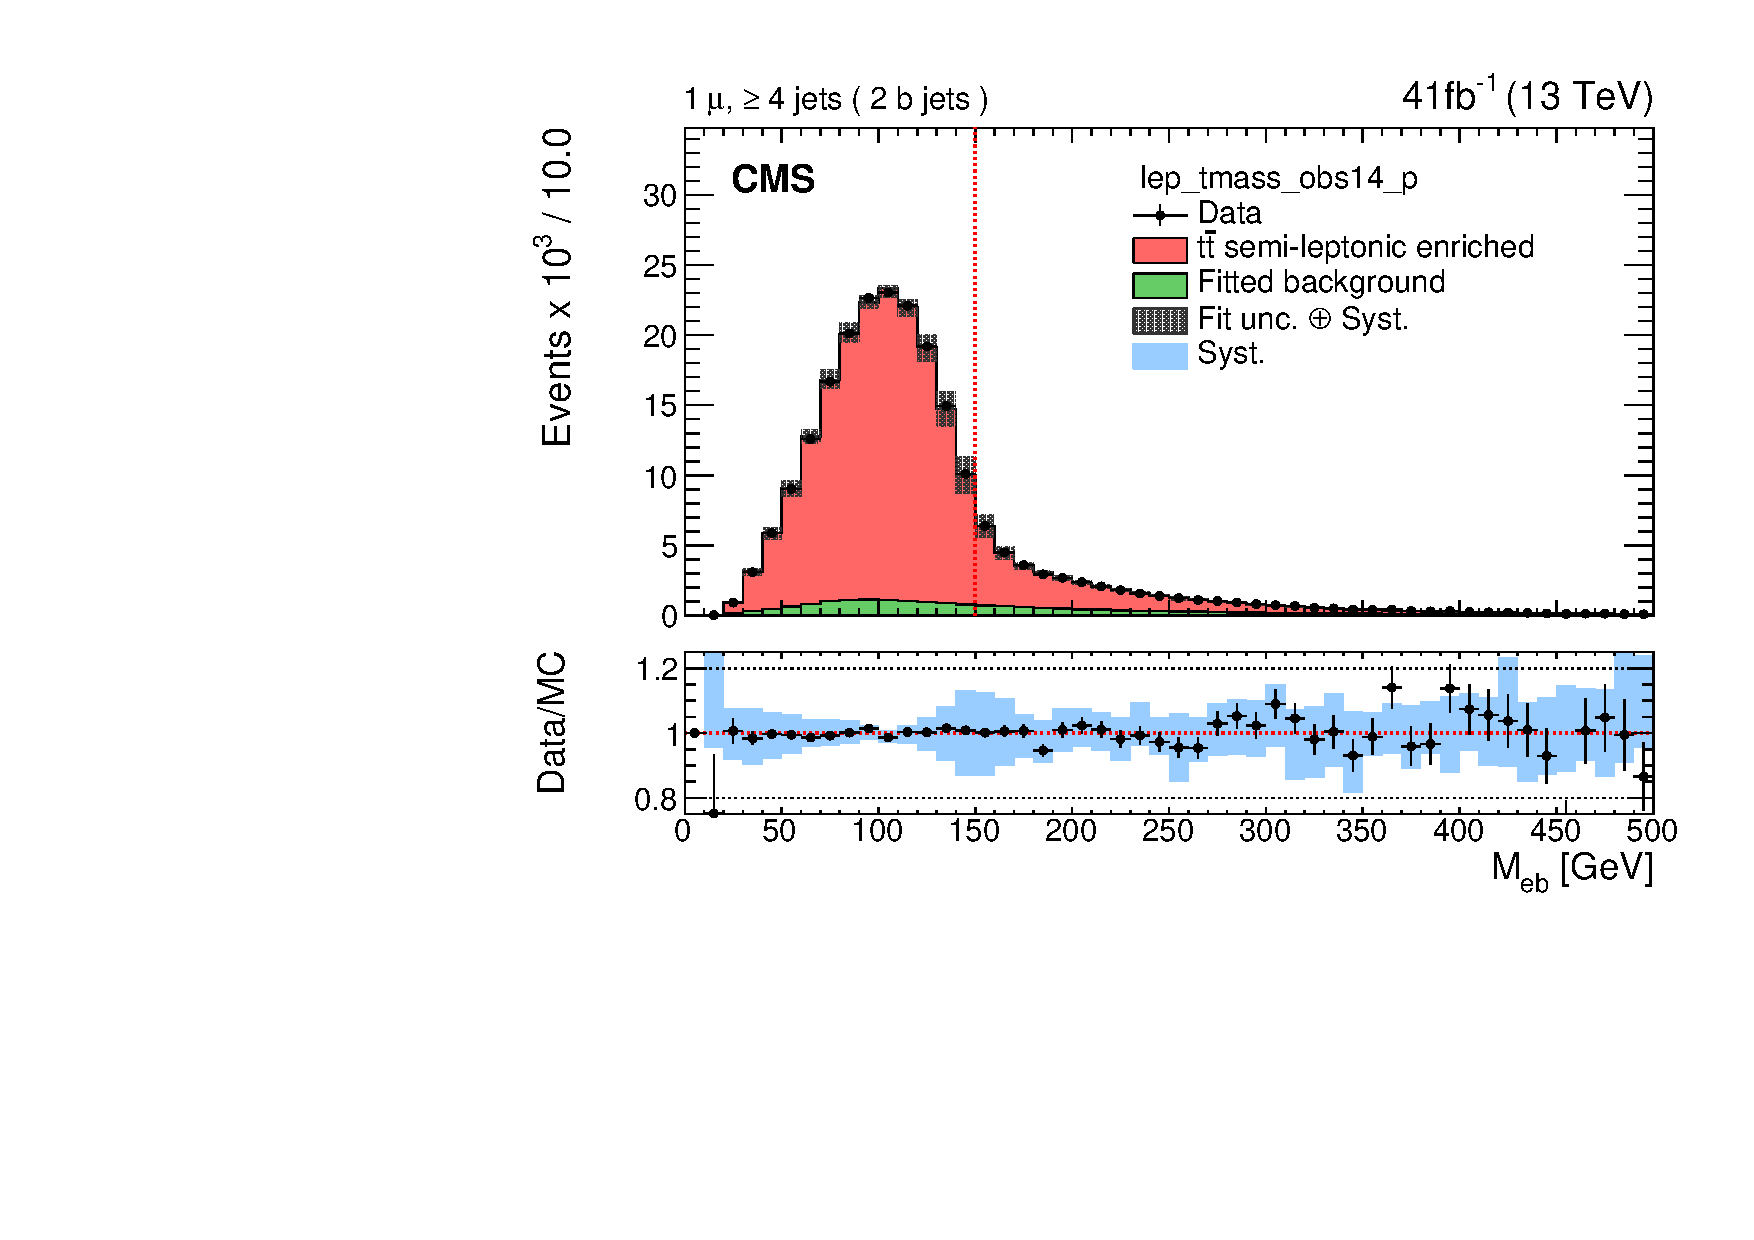
\includegraphics[width=0.4\textwidth]{figure/FitResult_17_mu_lep_tmass_obs14_p_chi2_20.pdf}
    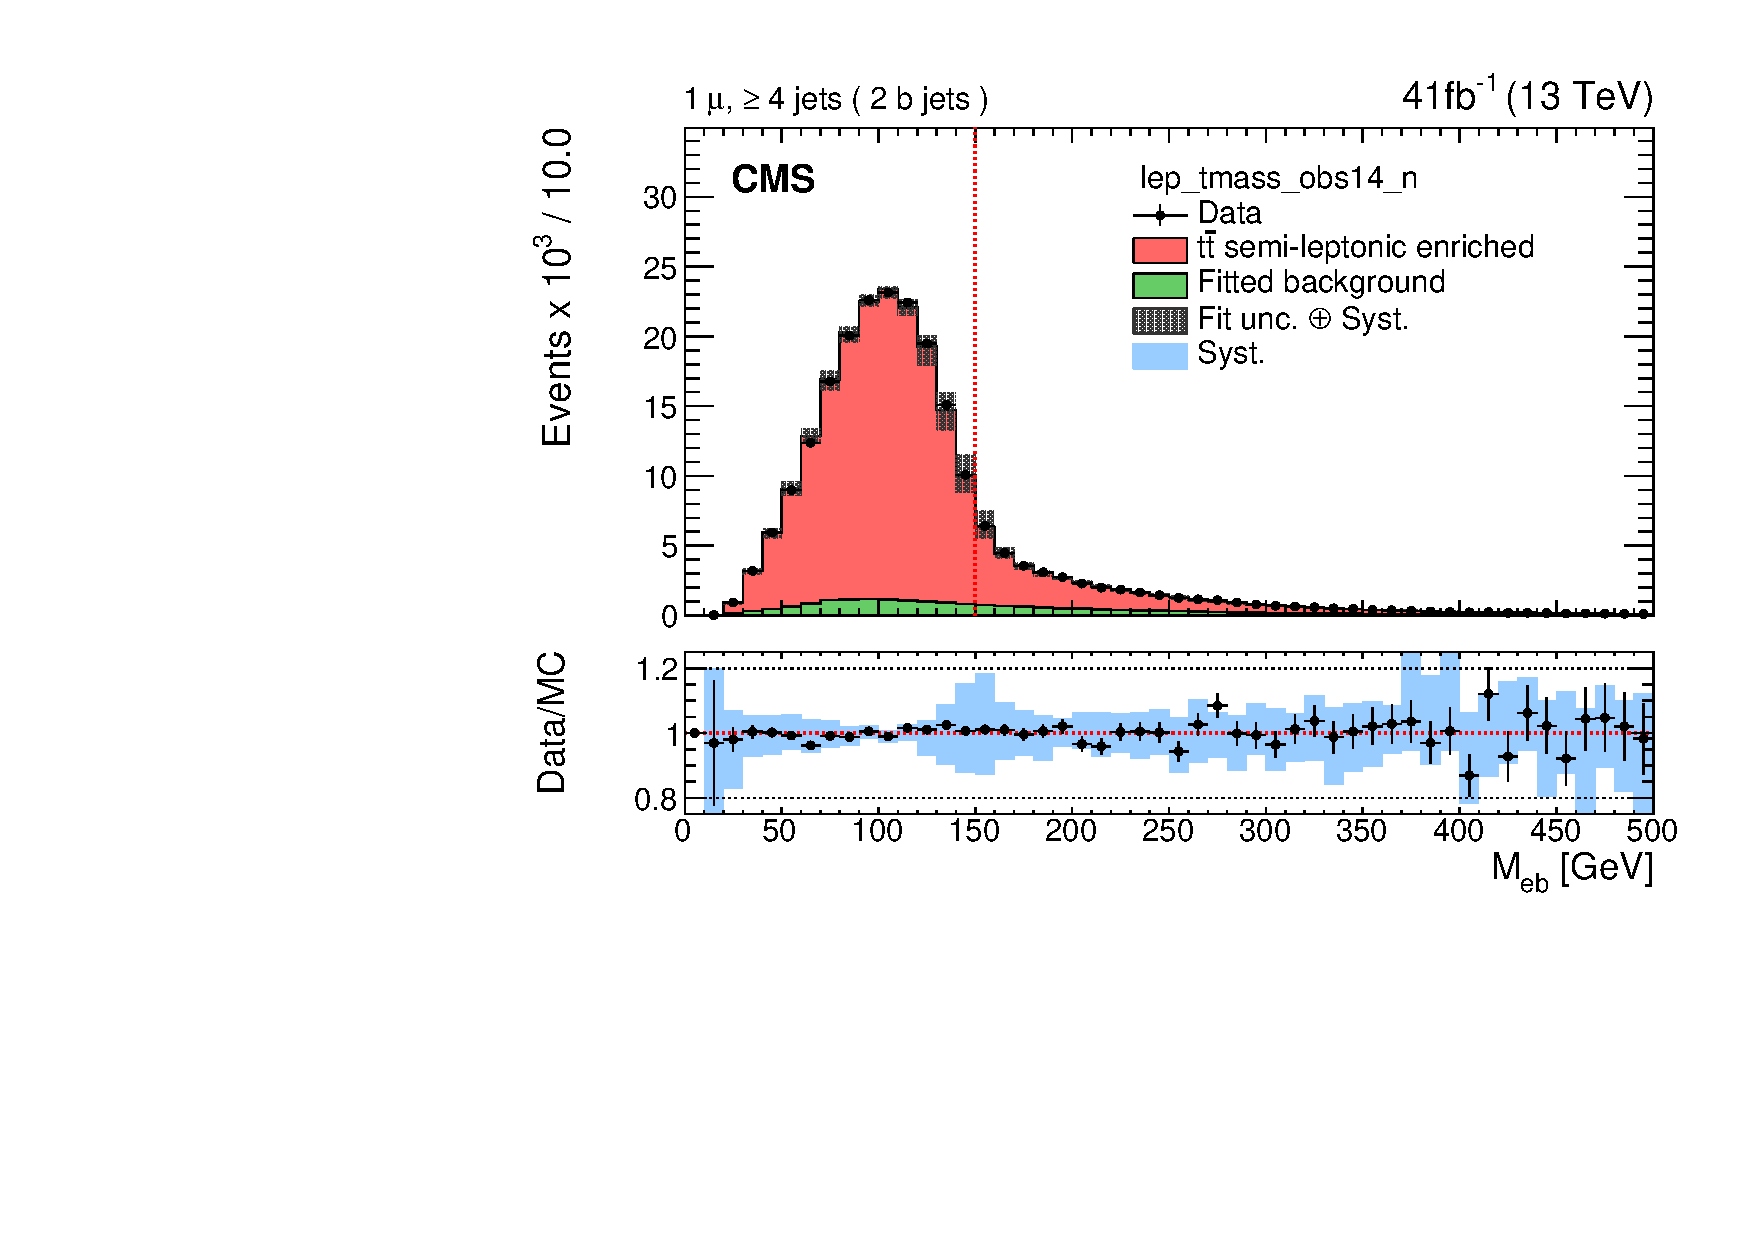
\includegraphics[width=0.4\textwidth]{figure/FitResult_17_mu_lep_tmass_obs14_n_chi2_20.pdf}
    \caption[The \Mlb invariant mass distributions in muon channel from 2017 data.]
    {
        The \Mlb invariant mass distributions in the positive (left) and negative (right) observable value region in muon channel from 2017 data (points).
        The results of the fit to the \ttbar and background templates are shown by the red and green histograms, respectively.
        The vertical bars on the data points in the upper panels indicate the statistical uncertainties in the data and the hatched bands show the combined statistical and systematic uncertainties in the simulation.
        The lower panels give the ratio of the data to the sum of the fitted MC predictions.
        The blue bands represent the systematic uncertainties in the expected yield in the simulation for all sources of systematic uncertainty (Section~\ref{sec:uncertainty}).
    }
    \label{fig:fitting_results_17_mu}
\end{figure}
\begin{figure}
    \centering
    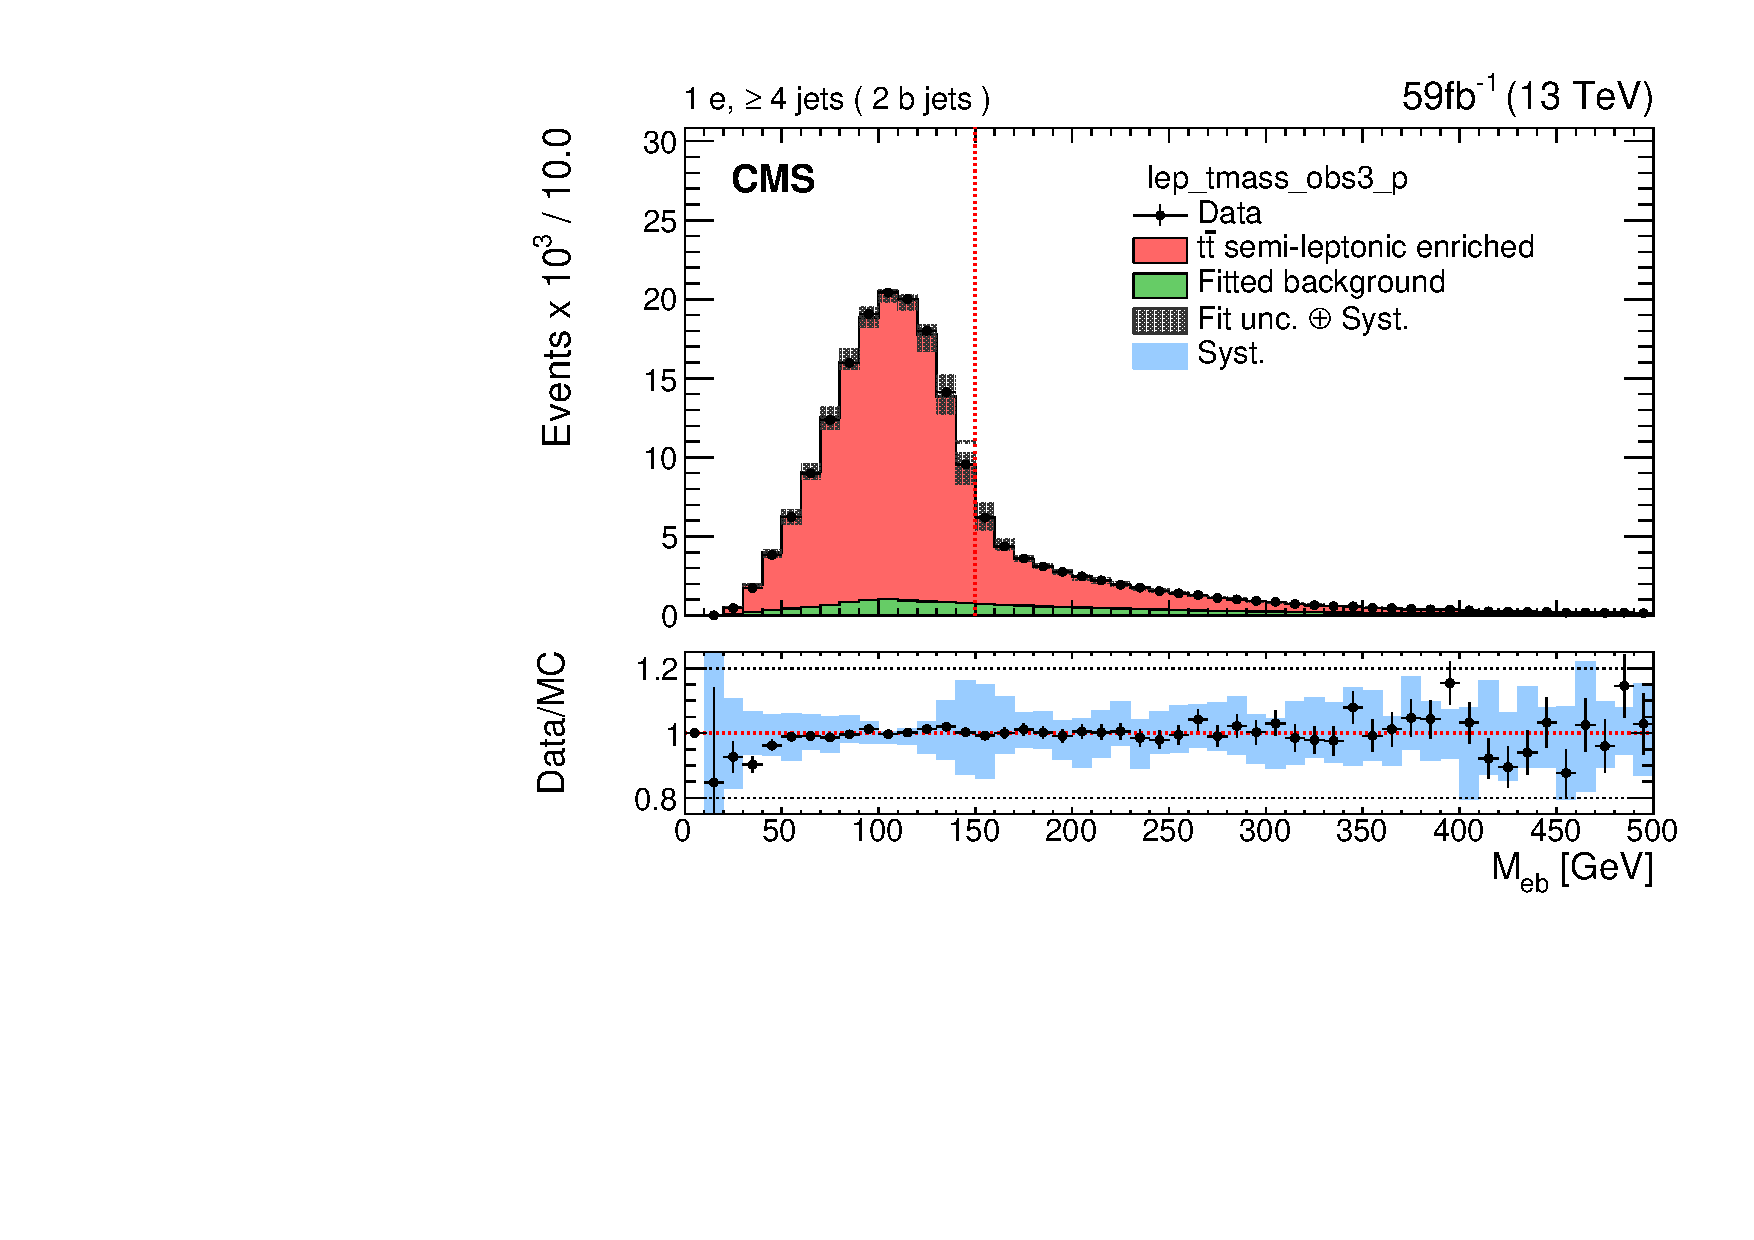
\includegraphics[width=0.4\textwidth]{figure/FitResult_18_el_lep_tmass_obs3_p_chi2_20.pdf}
    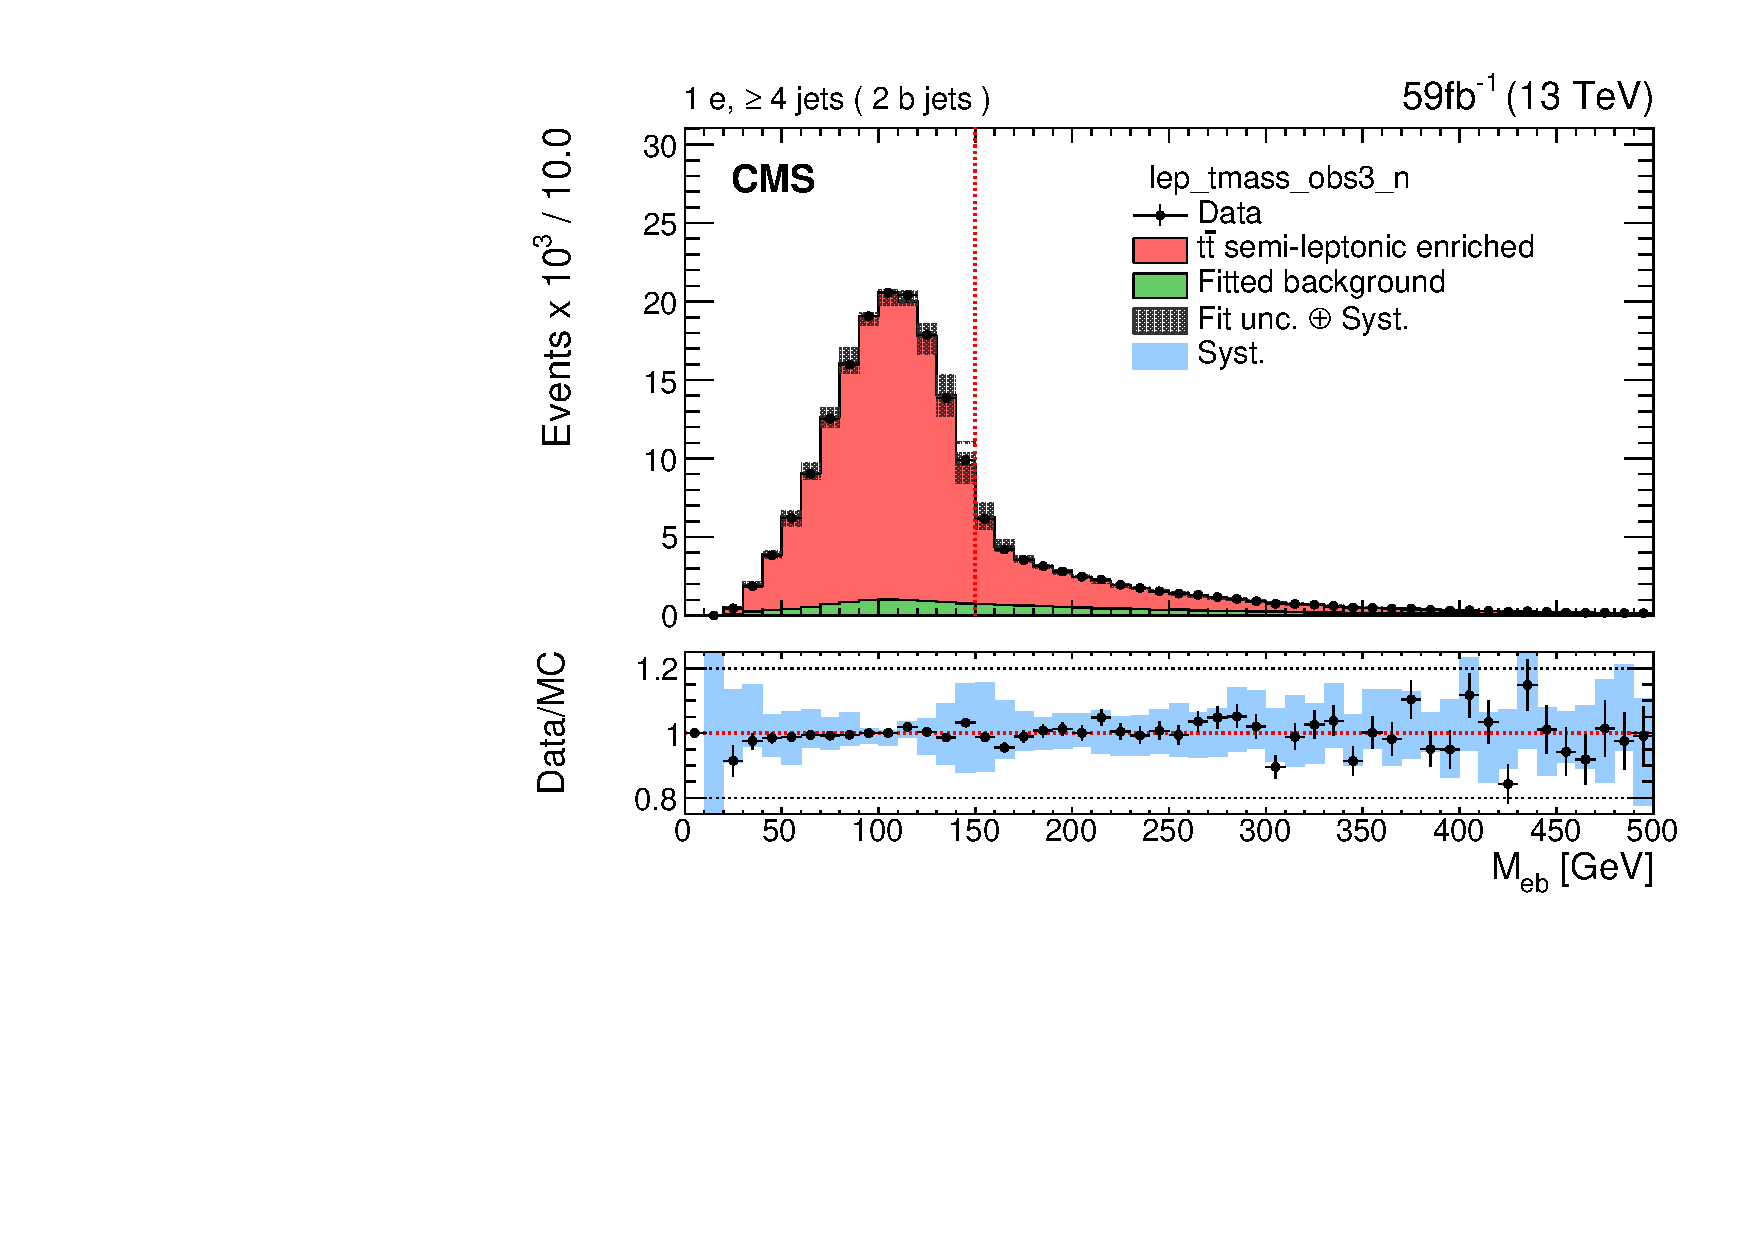
\includegraphics[width=0.4\textwidth]{figure/FitResult_18_el_lep_tmass_obs3_n_chi2_20.pdf}
    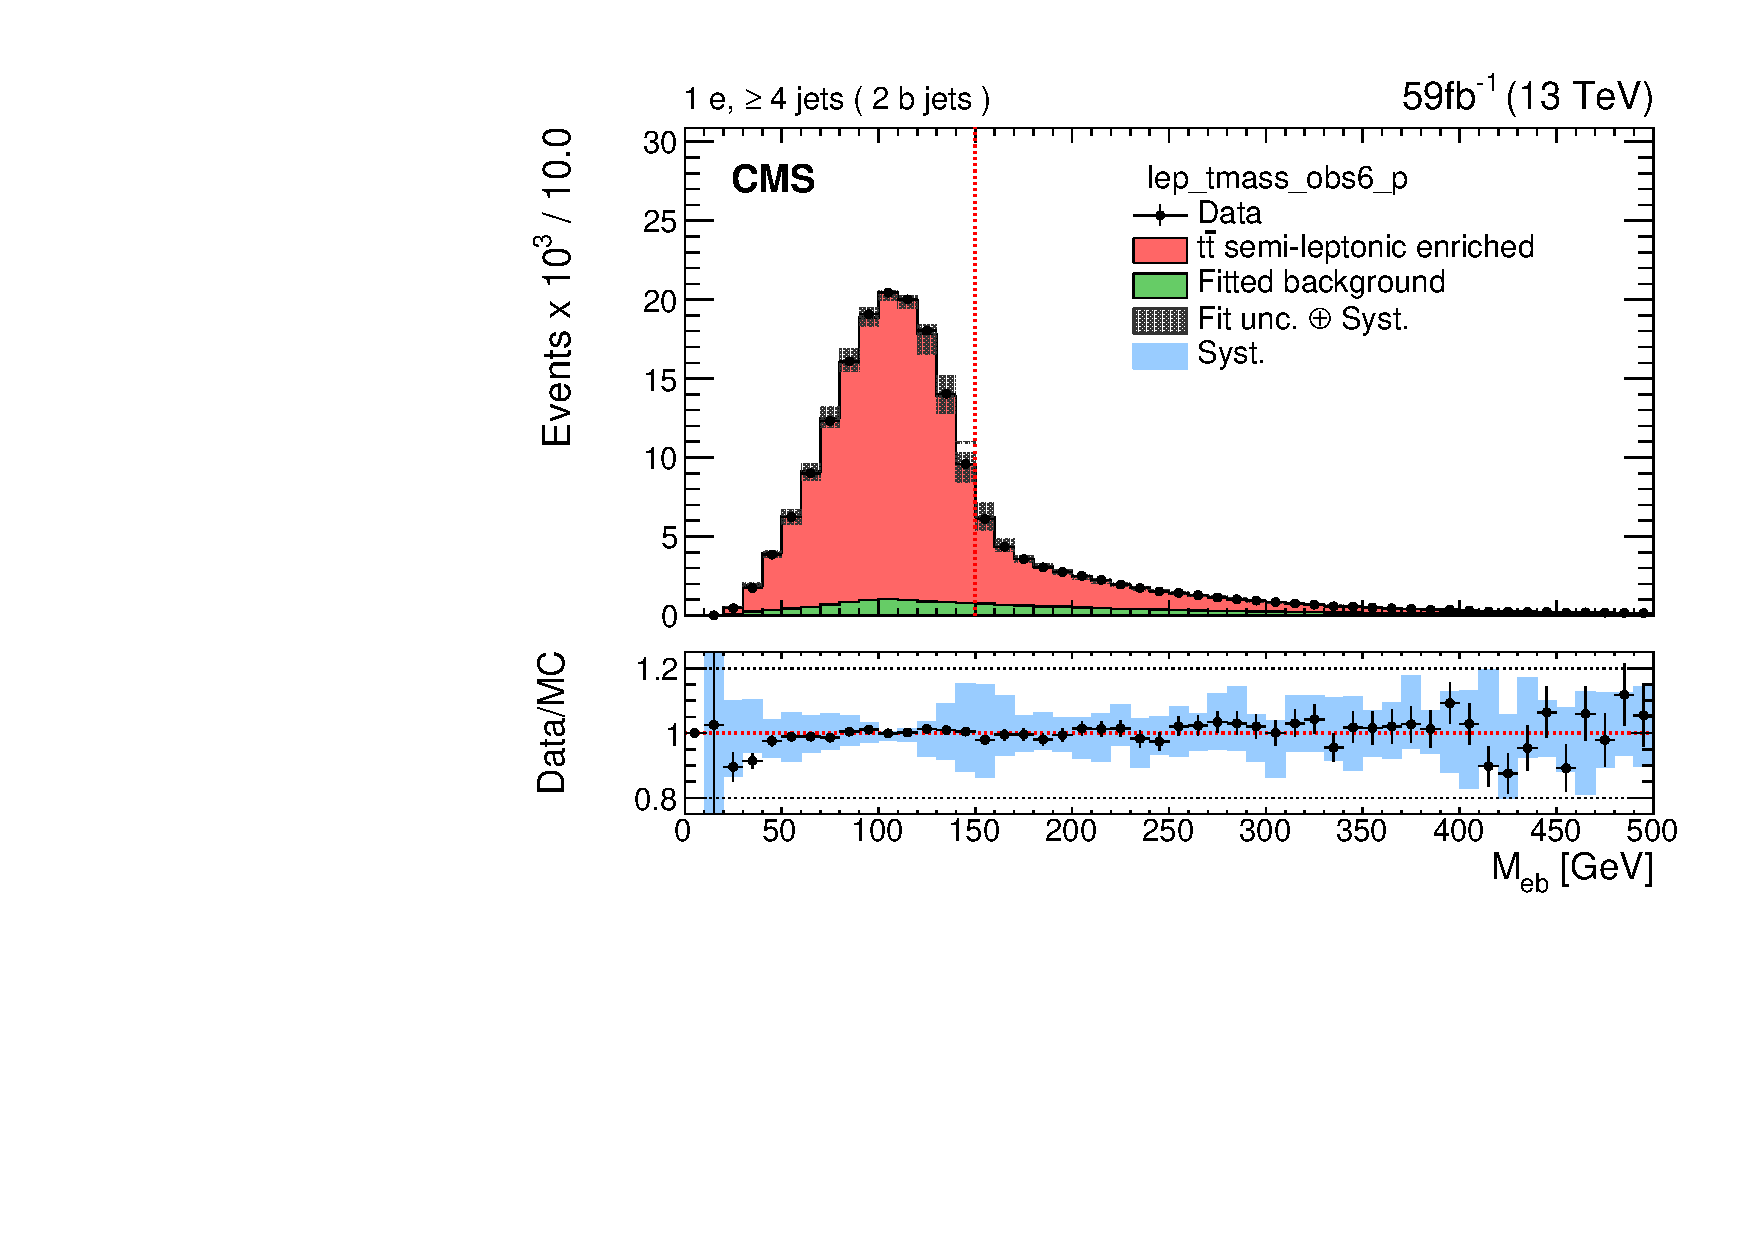
\includegraphics[width=0.4\textwidth]{figure/FitResult_18_el_lep_tmass_obs6_p_chi2_20.pdf}
    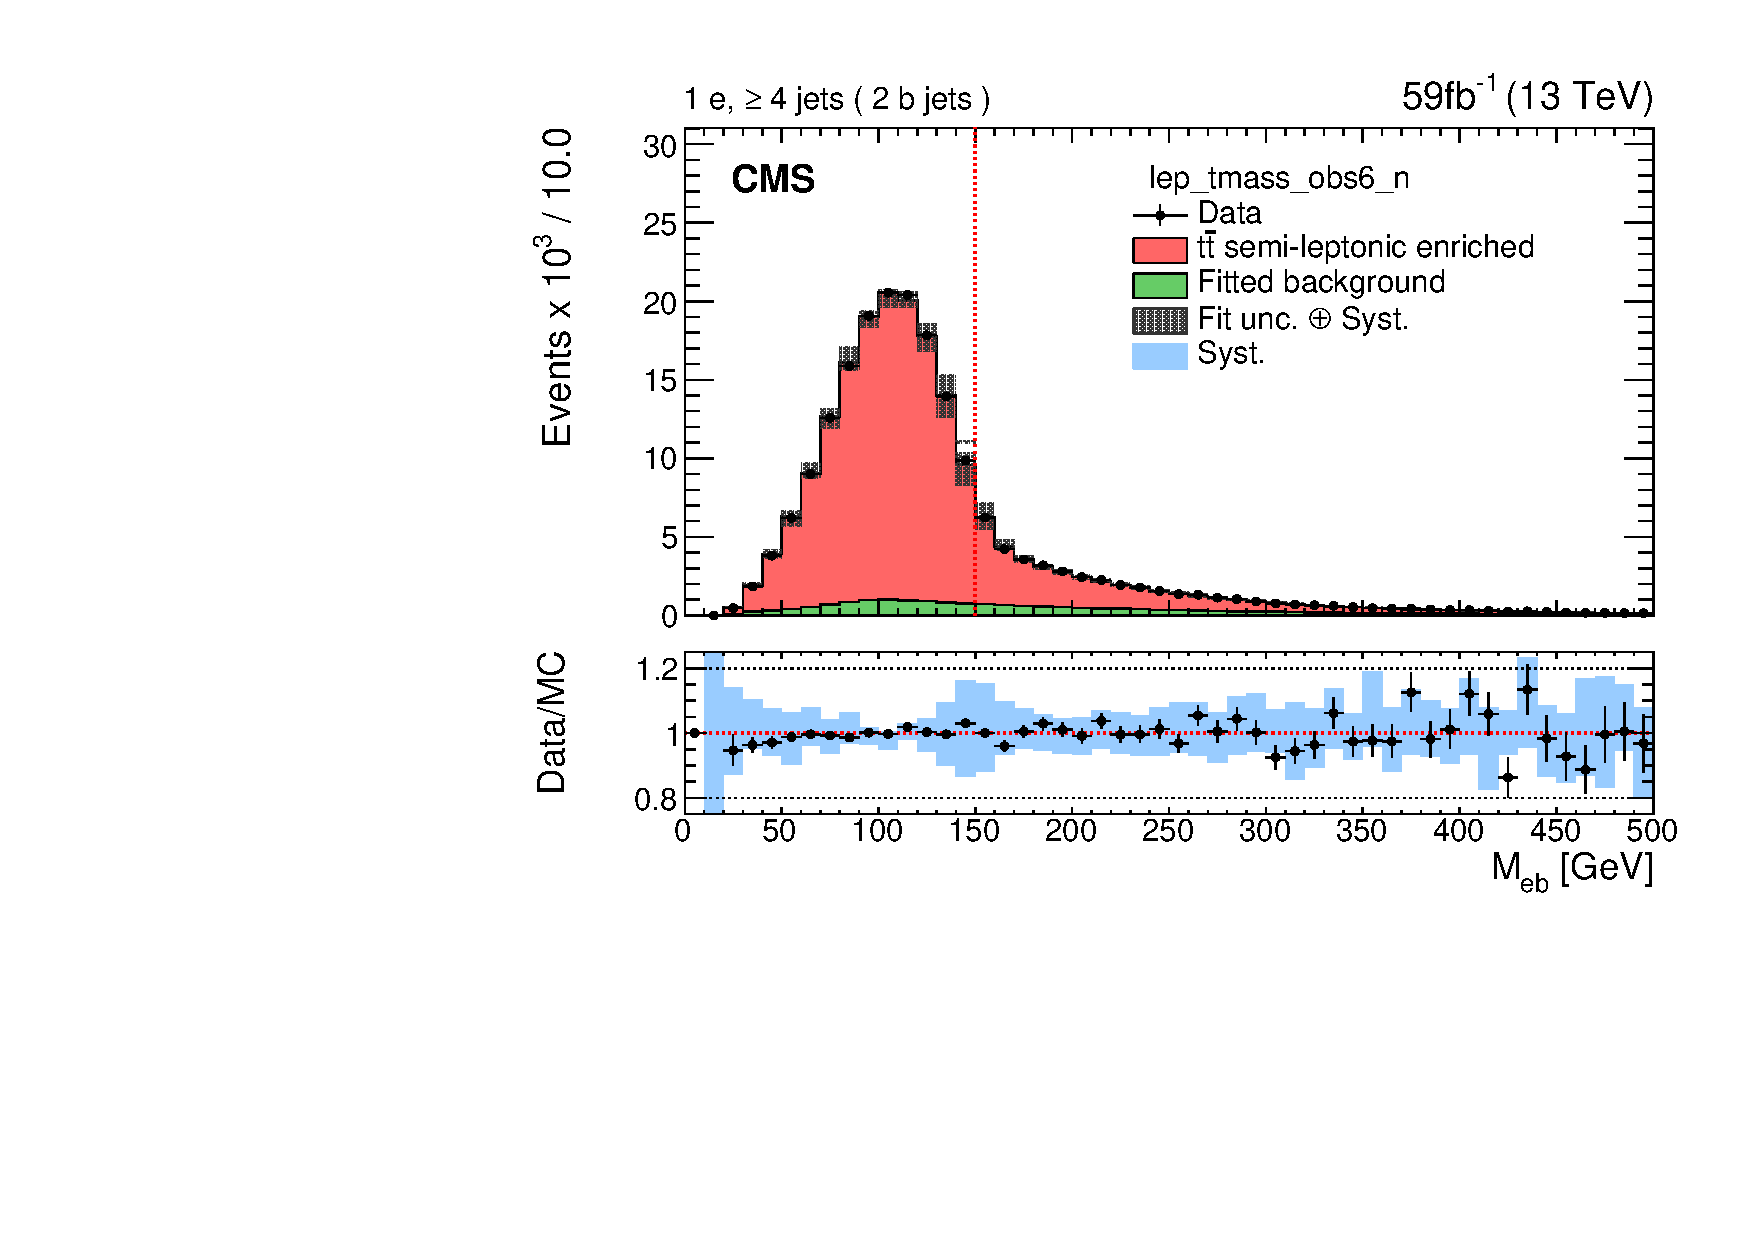
\includegraphics[width=0.4\textwidth]{figure/FitResult_18_el_lep_tmass_obs6_n_chi2_20.pdf}
    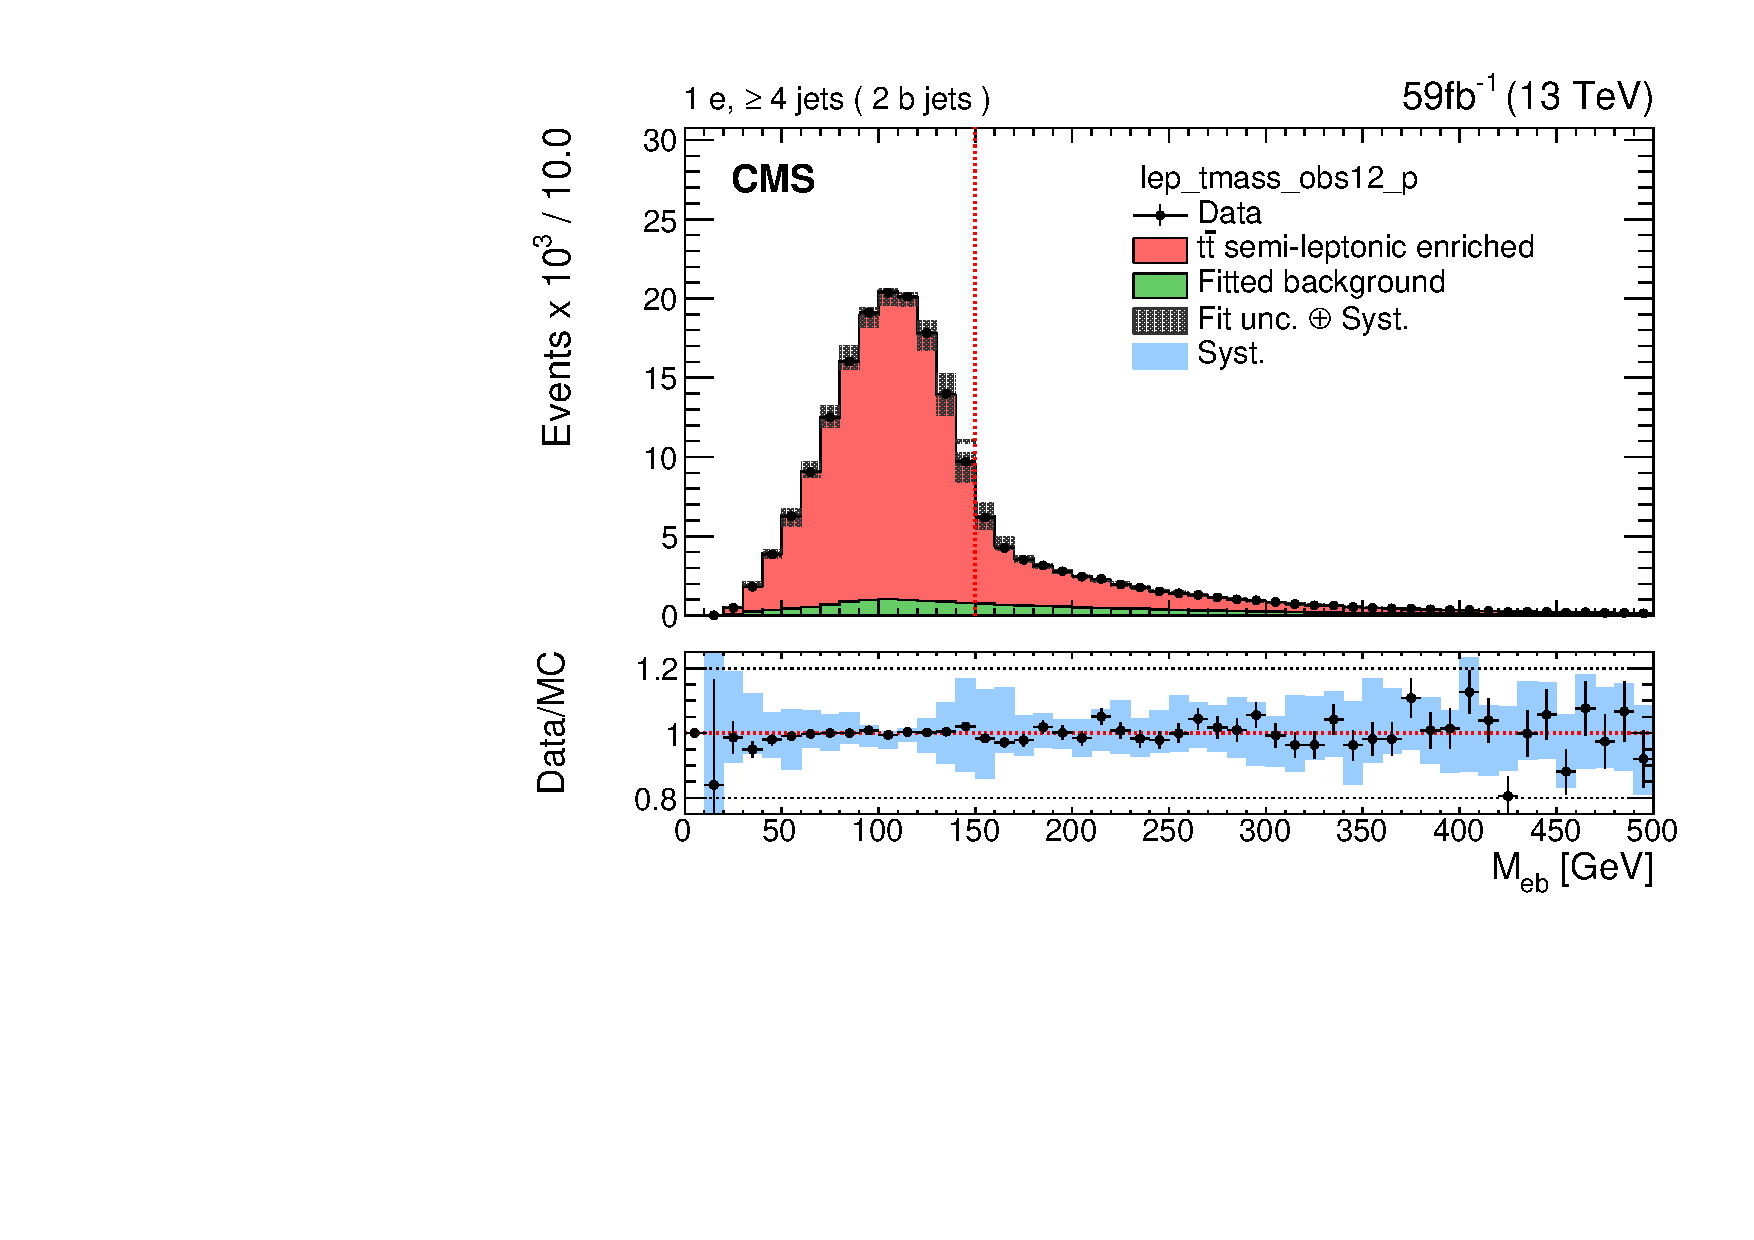
\includegraphics[width=0.4\textwidth]{figure/FitResult_18_el_lep_tmass_obs12_p_chi2_20.pdf}
    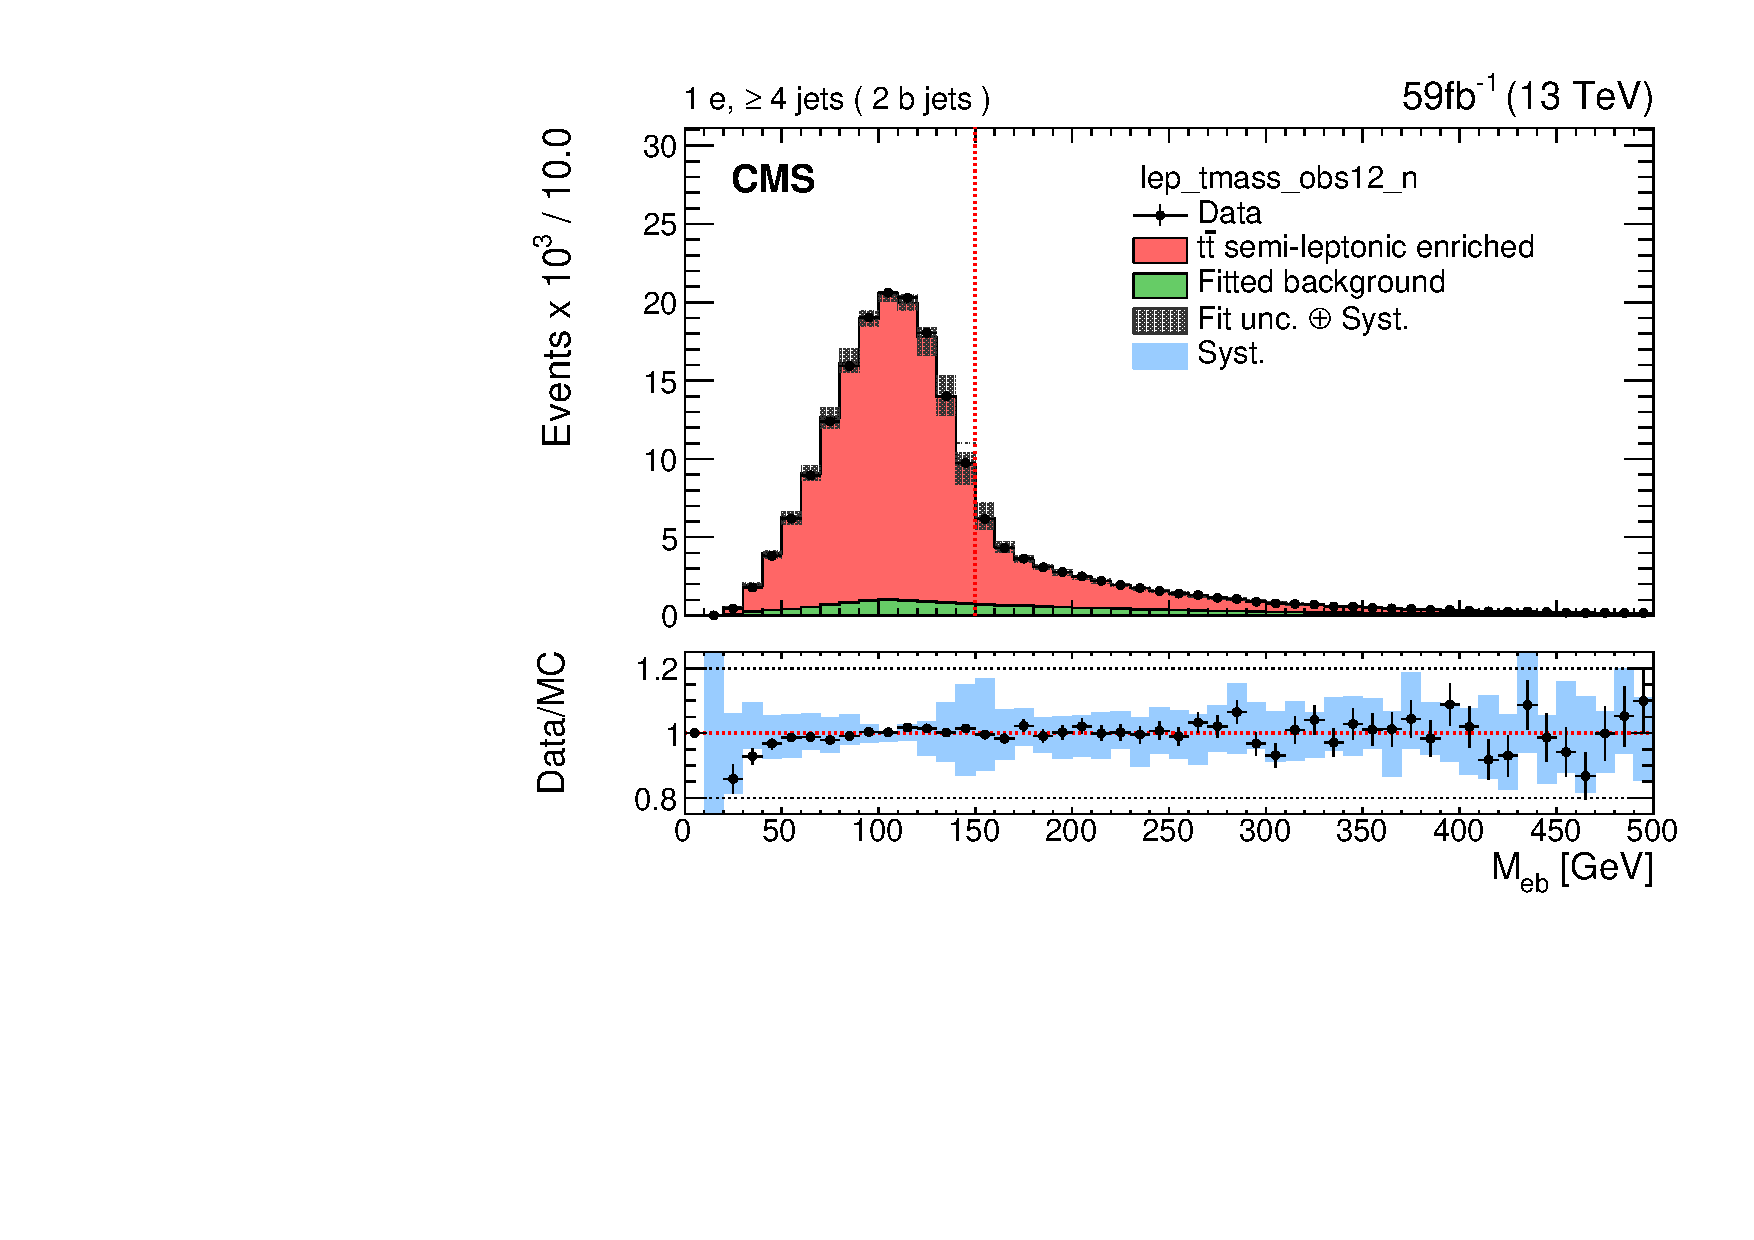
\includegraphics[width=0.4\textwidth]{figure/FitResult_18_el_lep_tmass_obs12_n_chi2_20.pdf}
    \includegraphics[width=0.4\textwidth]{figure/FitResult_18_el_lep_tmass_obs14_p_chi2_20.pdf}
    \includegraphics[width=0.4\textwidth]{figure/FitResult_18_el_lep_tmass_obs14_n_chi2_20.pdf}
    \caption[The \Mlb invariant mass distributions in electron channel from 2018 data.]
    {
        The \Mlb invariant mass distributions in the positive (left) and negative (right) observable value region in electron channel from 2018 data (points).
        The results of the fit to the \ttbar and background templates are shown by the red and green histograms, respectively.
        The vertical bars on the data points in the upper panels indicate the statistical uncertainties in the data and the hatched bands show the combined statistical and systematic uncertainties in the simulation.
        The lower panels give the ratio of the data to the sum of the fitted MC predictions.
        The blue bands represent the systematic uncertainties in the expected yield in the simulation for all sources of systematic uncertainty (Section~\ref{sec:uncertainty}).
    }
    \label{fig:fitting_results_18_el}
\end{figure}
\begin{figure}
    \centering
    \includegraphics[width=0.4\textwidth]{figure/FitResult_18_mu_lep_tmass_obs3_p_chi2_20.pdf}
    \includegraphics[width=0.4\textwidth]{figure/FitResult_18_mu_lep_tmass_obs3_n_chi2_20.pdf}
    \includegraphics[width=0.4\textwidth]{figure/FitResult_18_mu_lep_tmass_obs6_p_chi2_20.pdf}
    \includegraphics[width=0.4\textwidth]{figure/FitResult_18_mu_lep_tmass_obs6_n_chi2_20.pdf}
    \includegraphics[width=0.4\textwidth]{figure/FitResult_18_mu_lep_tmass_obs12_p_chi2_20.pdf}
    \includegraphics[width=0.4\textwidth]{figure/FitResult_18_mu_lep_tmass_obs12_n_chi2_20.pdf}
    \includegraphics[width=0.4\textwidth]{figure/FitResult_18_mu_lep_tmass_obs14_p_chi2_20.pdf}
    \includegraphics[width=0.4\textwidth]{figure/FitResult_18_mu_lep_tmass_obs14_n_chi2_20.pdf}
    \caption[The \Mlb invariant mass distributions in muon channel from 2018 data.]
    {
        The \Mlb invariant mass distributions in the positive (left) and negative (right) observable value region in muon channel from 2018 data (points).
        The results of the fit to the \ttbar and background templates are shown by the red and green histograms, respectively.
        The vertical bars on the data points in the upper panels indicate the statistical uncertainties in the data and the hatched bands show the combined statistical and systematic uncertainties in the simulation.
        The lower panels give the ratio of the data to the sum of the fitted MC predictions.
        The blue bands represent the systematic uncertainties in the expected yield in the simulation for all sources of systematic uncertainty (Section~\ref{sec:uncertainty}).
    }
    \label{fig:fitting_results_18_mu}
\end{figure}

\begin{table}
    \caption[The fitted number of \ttbar signal and \ttbar background events and other background events.]
    {
        The fitted number of \ttbar signal and \ttbar background events (fitted \ttbar) and other background events (fitted background) in the electron and muon channels, along with the \ttbar purities.
        Although the fit is performed for $\Mlb < 500\GeV$, the event yields are given for $\Mlb < 150\GeV$.
        The uncertainties shown are statistical only.
    }
    \label{tab:fitting_purity}
    \centering\renewcommand\arraystretch{1.2}
    \begin{tabular}{ccc}
        & Electron channel & Muon channel\\
        \hline
        Fitted \ttbar & $604\,700 \pm 1200$ & $1\,062\,600 \pm 1500$\\
        Fitted background & $34\,030 \pm 480$ & $58\,490 \pm 820$\\
        Fitted fraction of \ttbar (\%) & $94.7 \pm 0.1$ & $94.8 \pm 0.1$ \\
    \end{tabular}
\end{table}



